%%%%%%%%%%%%%%%%%%%%%%%%%%%%%%%%%%%%%%%%%%%%%%%%%%%%%%%%%%%
\begin{frame}[fragile]\frametitle{Sequence-to-Sequence (seq2seq)}

\begin{center}
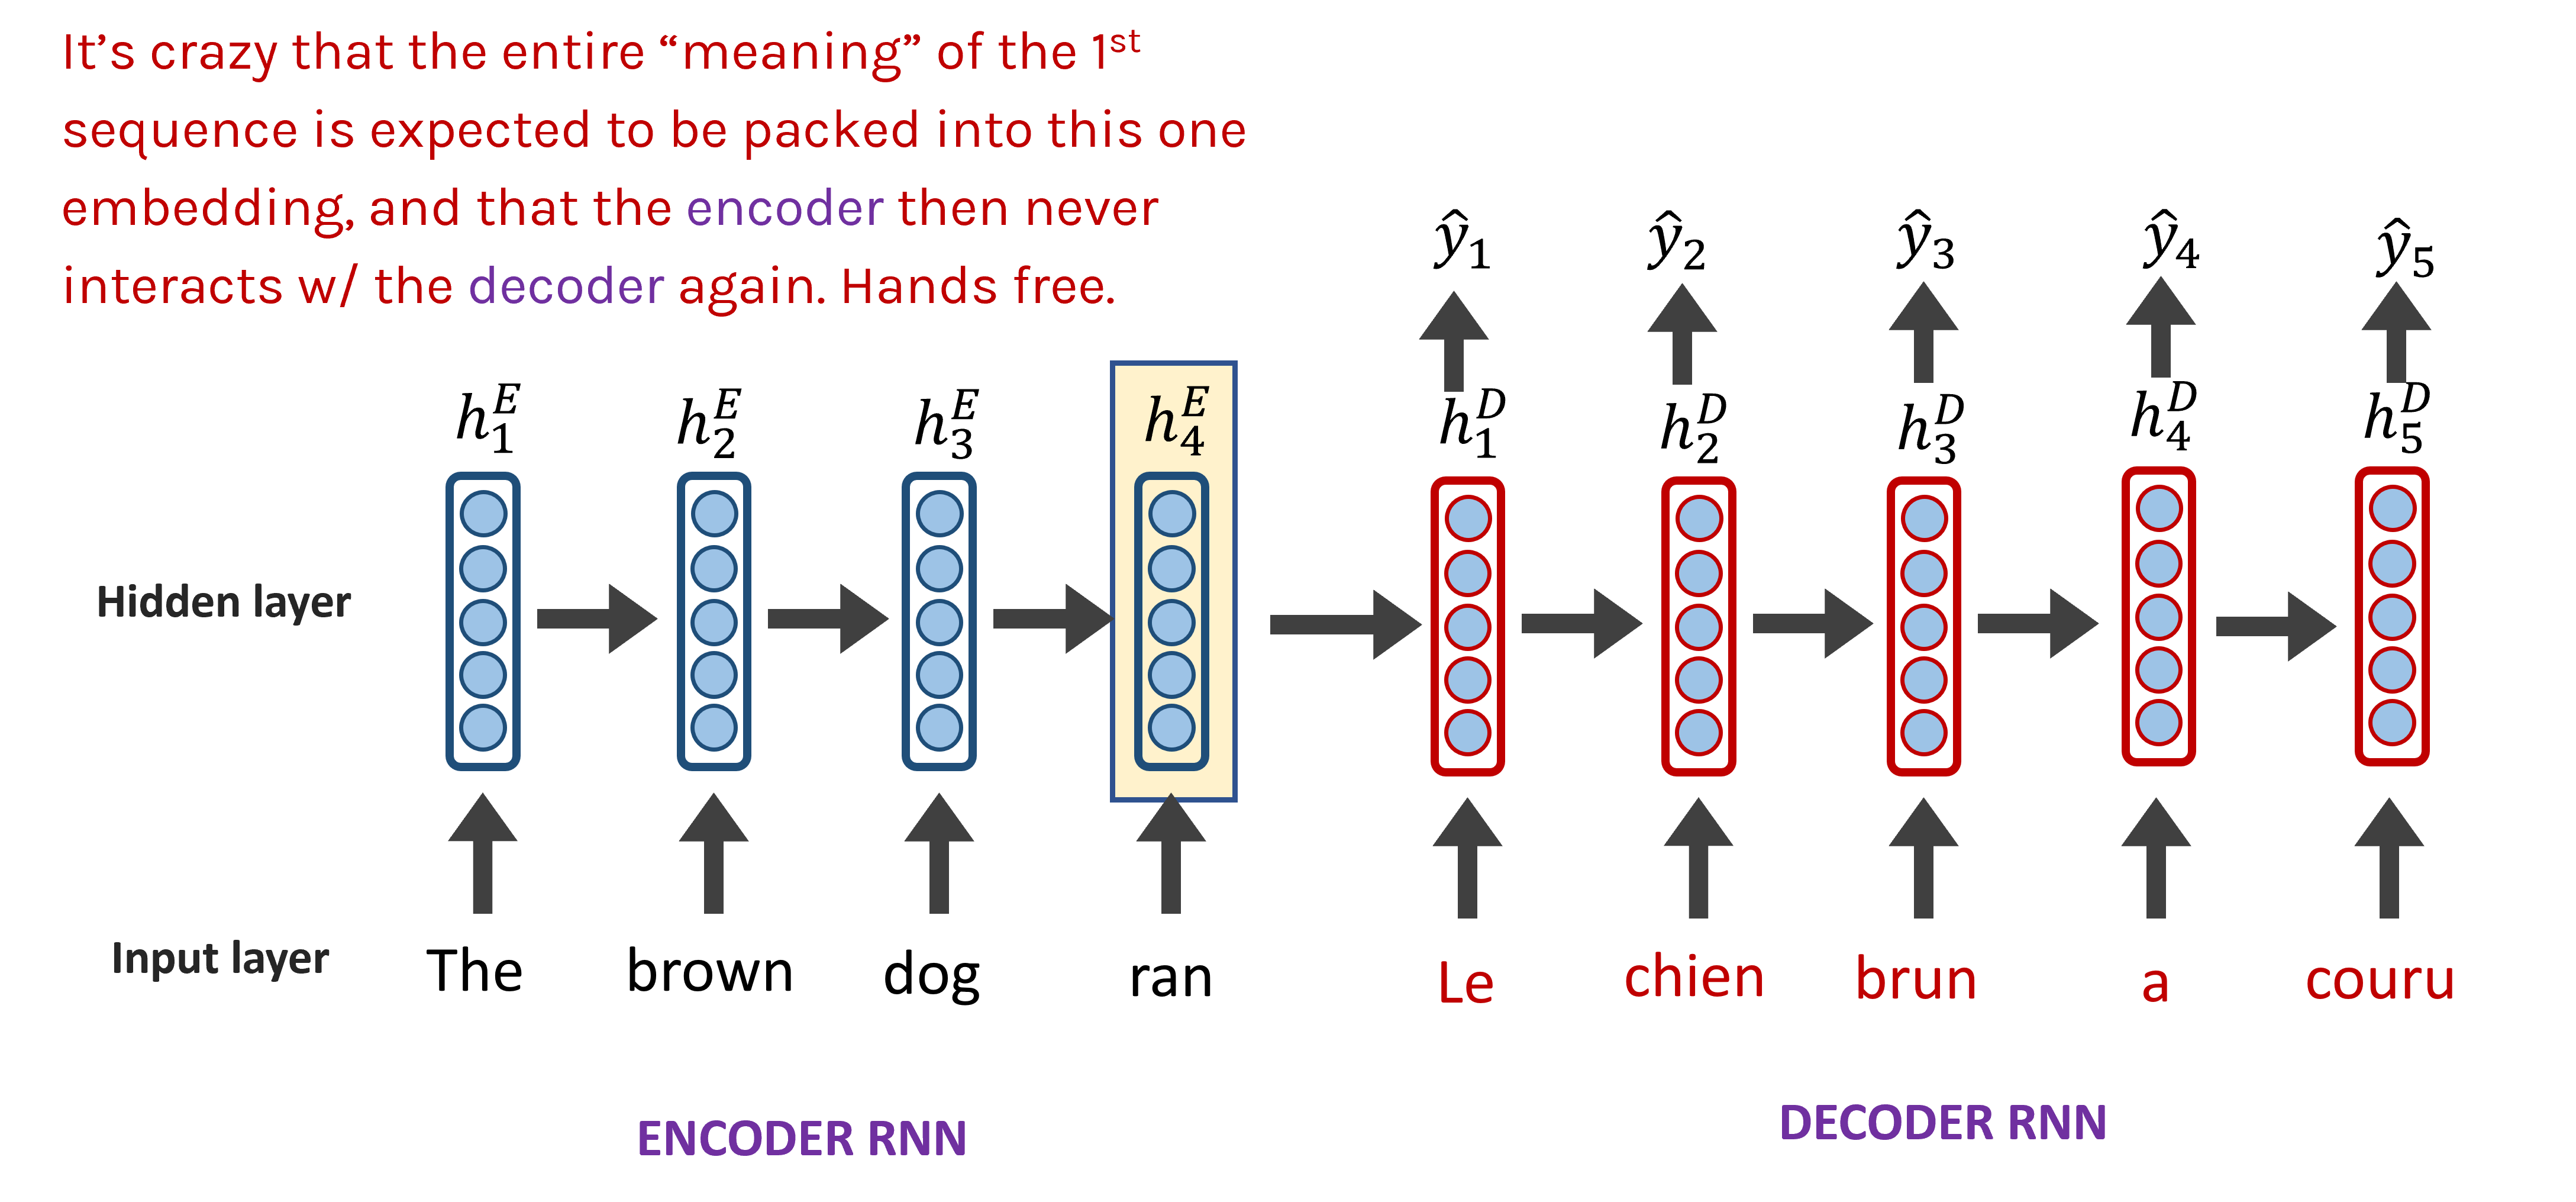
\includegraphics[width=\linewidth,keepaspectratio]{bert14}
\end{center}	

\end{frame}

%%%%%%%%%%%%%%%%%%%%%%%%%%%%%%%%%%%%%%%%%%%%%%%%%%%%%%%%%%%
\begin{frame}[fragile]\frametitle{Sequence-to-Sequence (seq2seq)}

\begin{center}
Instead, what if the decoder, at each step, pays {\bf attention} to a distribution of all of the encoder’s hidden states?
\end{center}	

\end{frame}

%%%%%%%%%%%%%%%%%%%%%%%%%%%%%%%%%%%%%%%%%%%%%%%%%%%%%%%%%%%
\begin{frame}[fragile]\frametitle{seq2seq + Attention}

Q: How do we determine how much to pay attention to each of the encoder’s hidden layers? 

\begin{center}
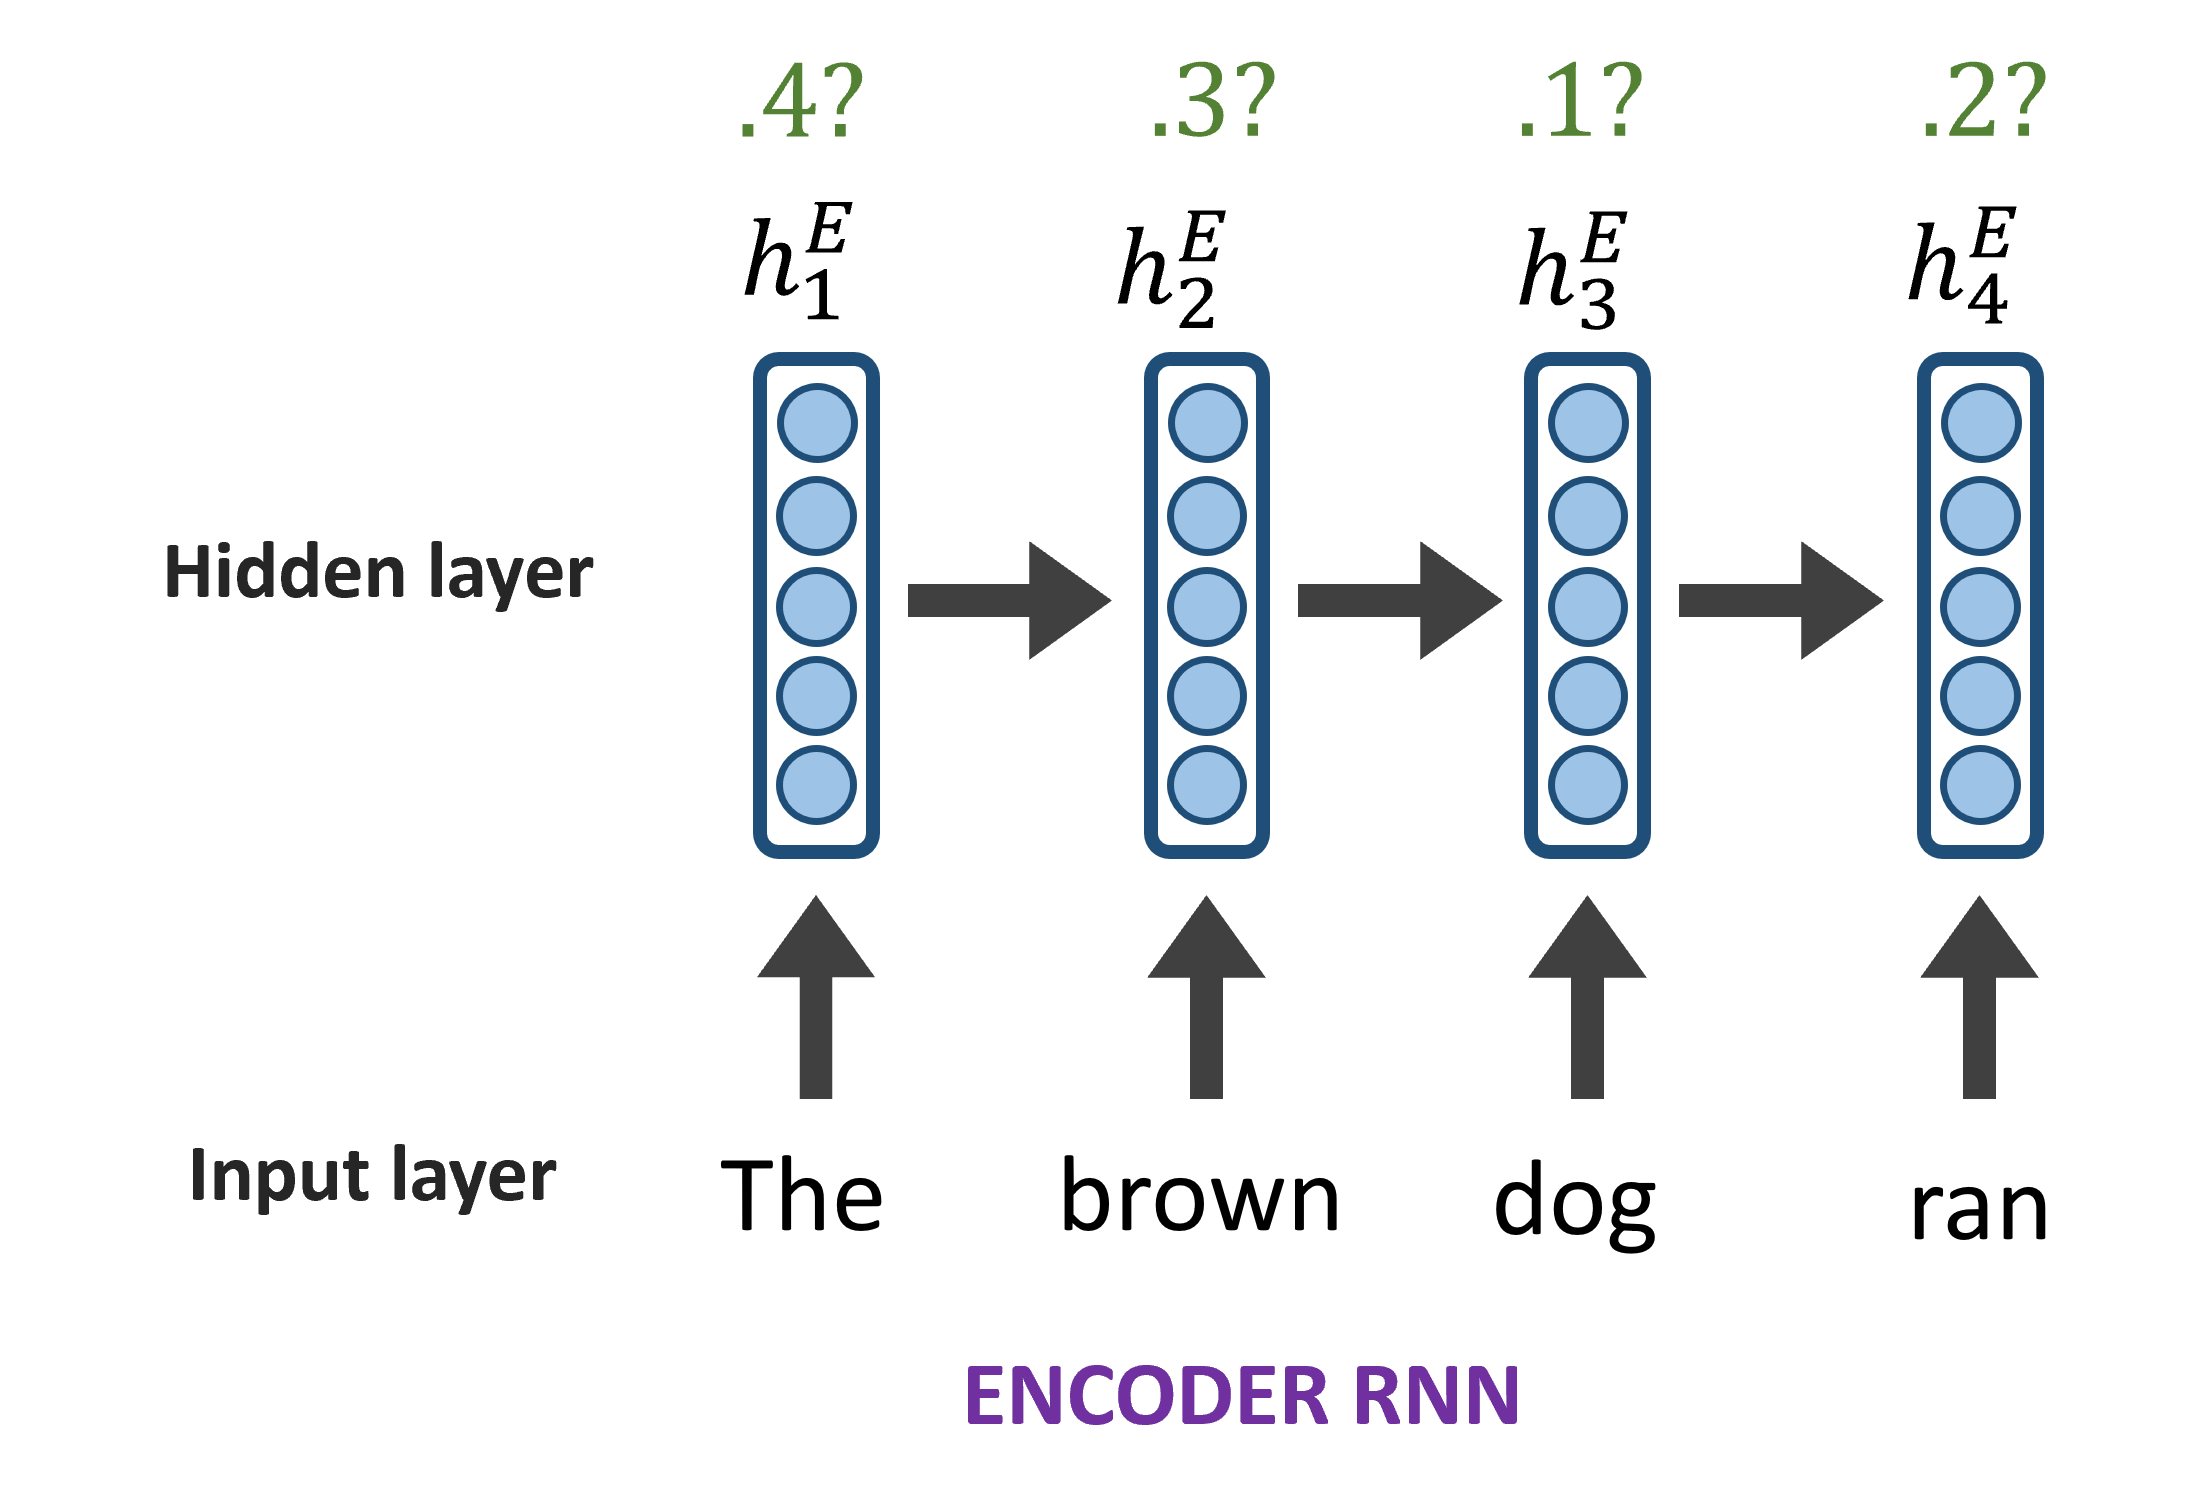
\includegraphics[width=0.8\linewidth,keepaspectratio]{bert15}
\end{center}	

\end{frame}


%%%%%%%%%%%%%%%%%%%%%%%%%%%%%%%%%%%%%%%%%%%%%%%%%%%%%%%%%%%
\begin{frame}[fragile]\frametitle{seq2seq + Attention}

Q: How do we determine how much to pay attention to each of the encoder’s hidden layers? 

A: Let’s base it on our decoder’s previous hidden state (our latest representation of meaning) and all of the encoder’s hidden layers!


\begin{center}
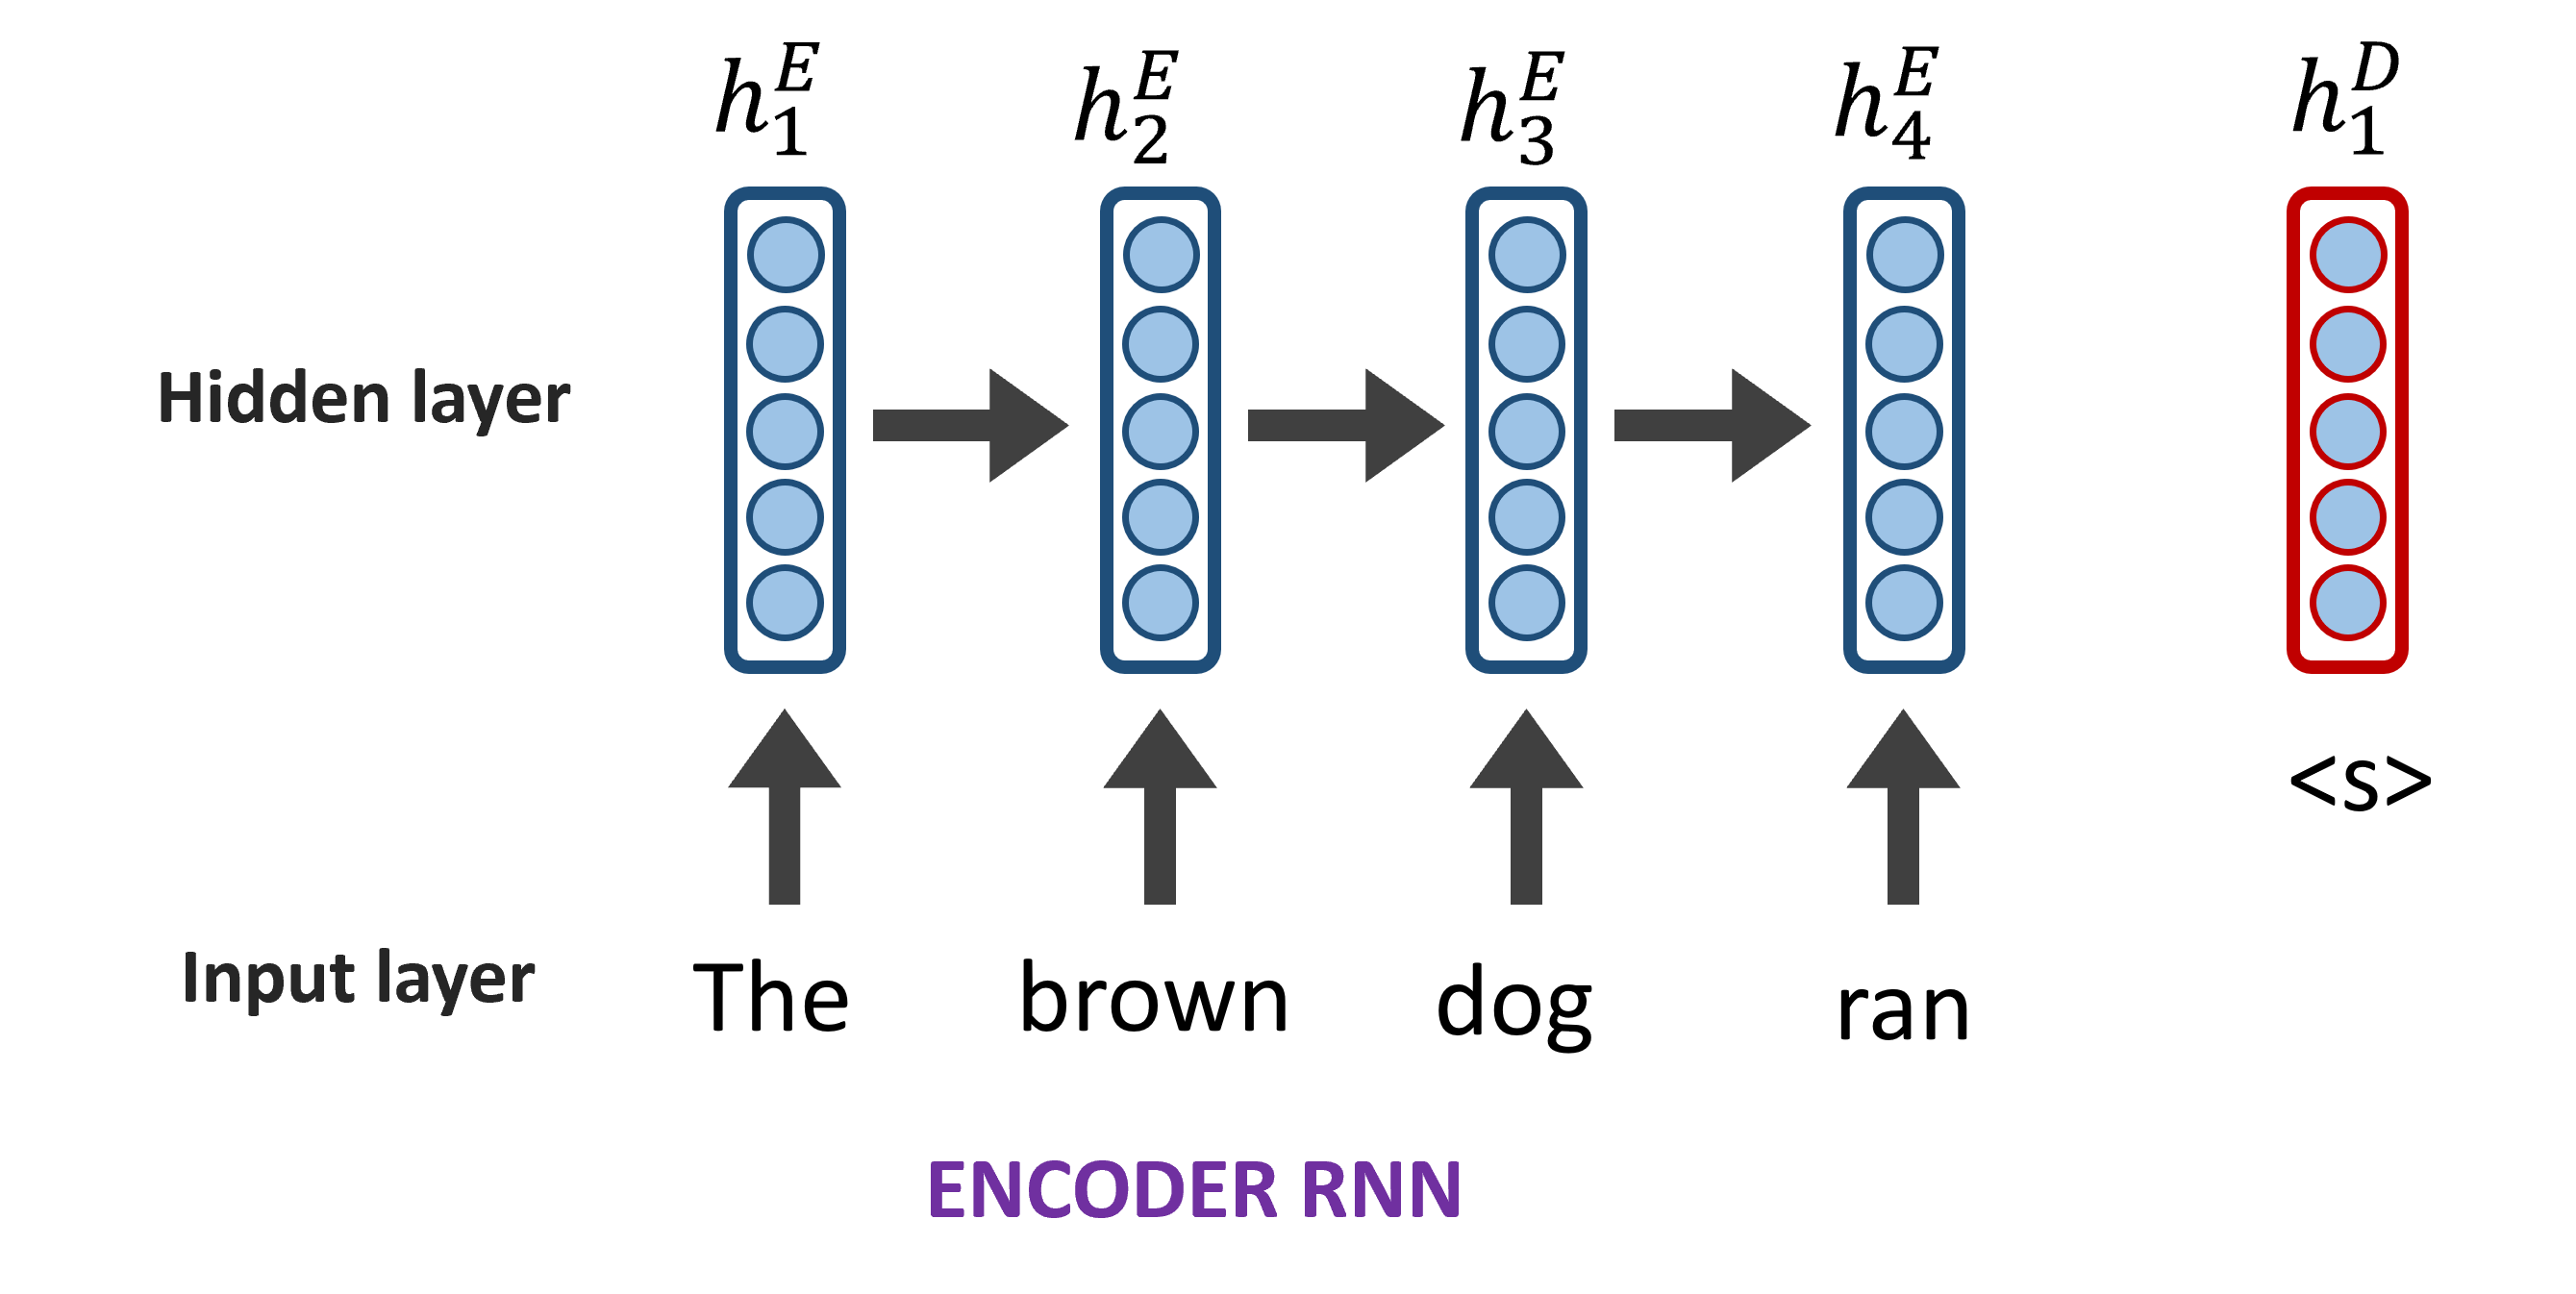
\includegraphics[width=0.8\linewidth,keepaspectratio]{bert16}
\end{center}	

\end{frame}

% %%%%%%%%%%%%%%%%%%%%%%%%%%%%%%%%%%%%%%%%%%%%%%%%%%%%%%%%%%%
% \begin{frame}[fragile]\frametitle{seq2seq + Attention}

% Q: How do we determine how much to pay attention to each of the encoder’s hidden layers? 

% A: Let’s base it on our decoder’s previous hidden state (our latest representation of meaning) and all of the encoder’s hidden layers!


% \begin{center}
% 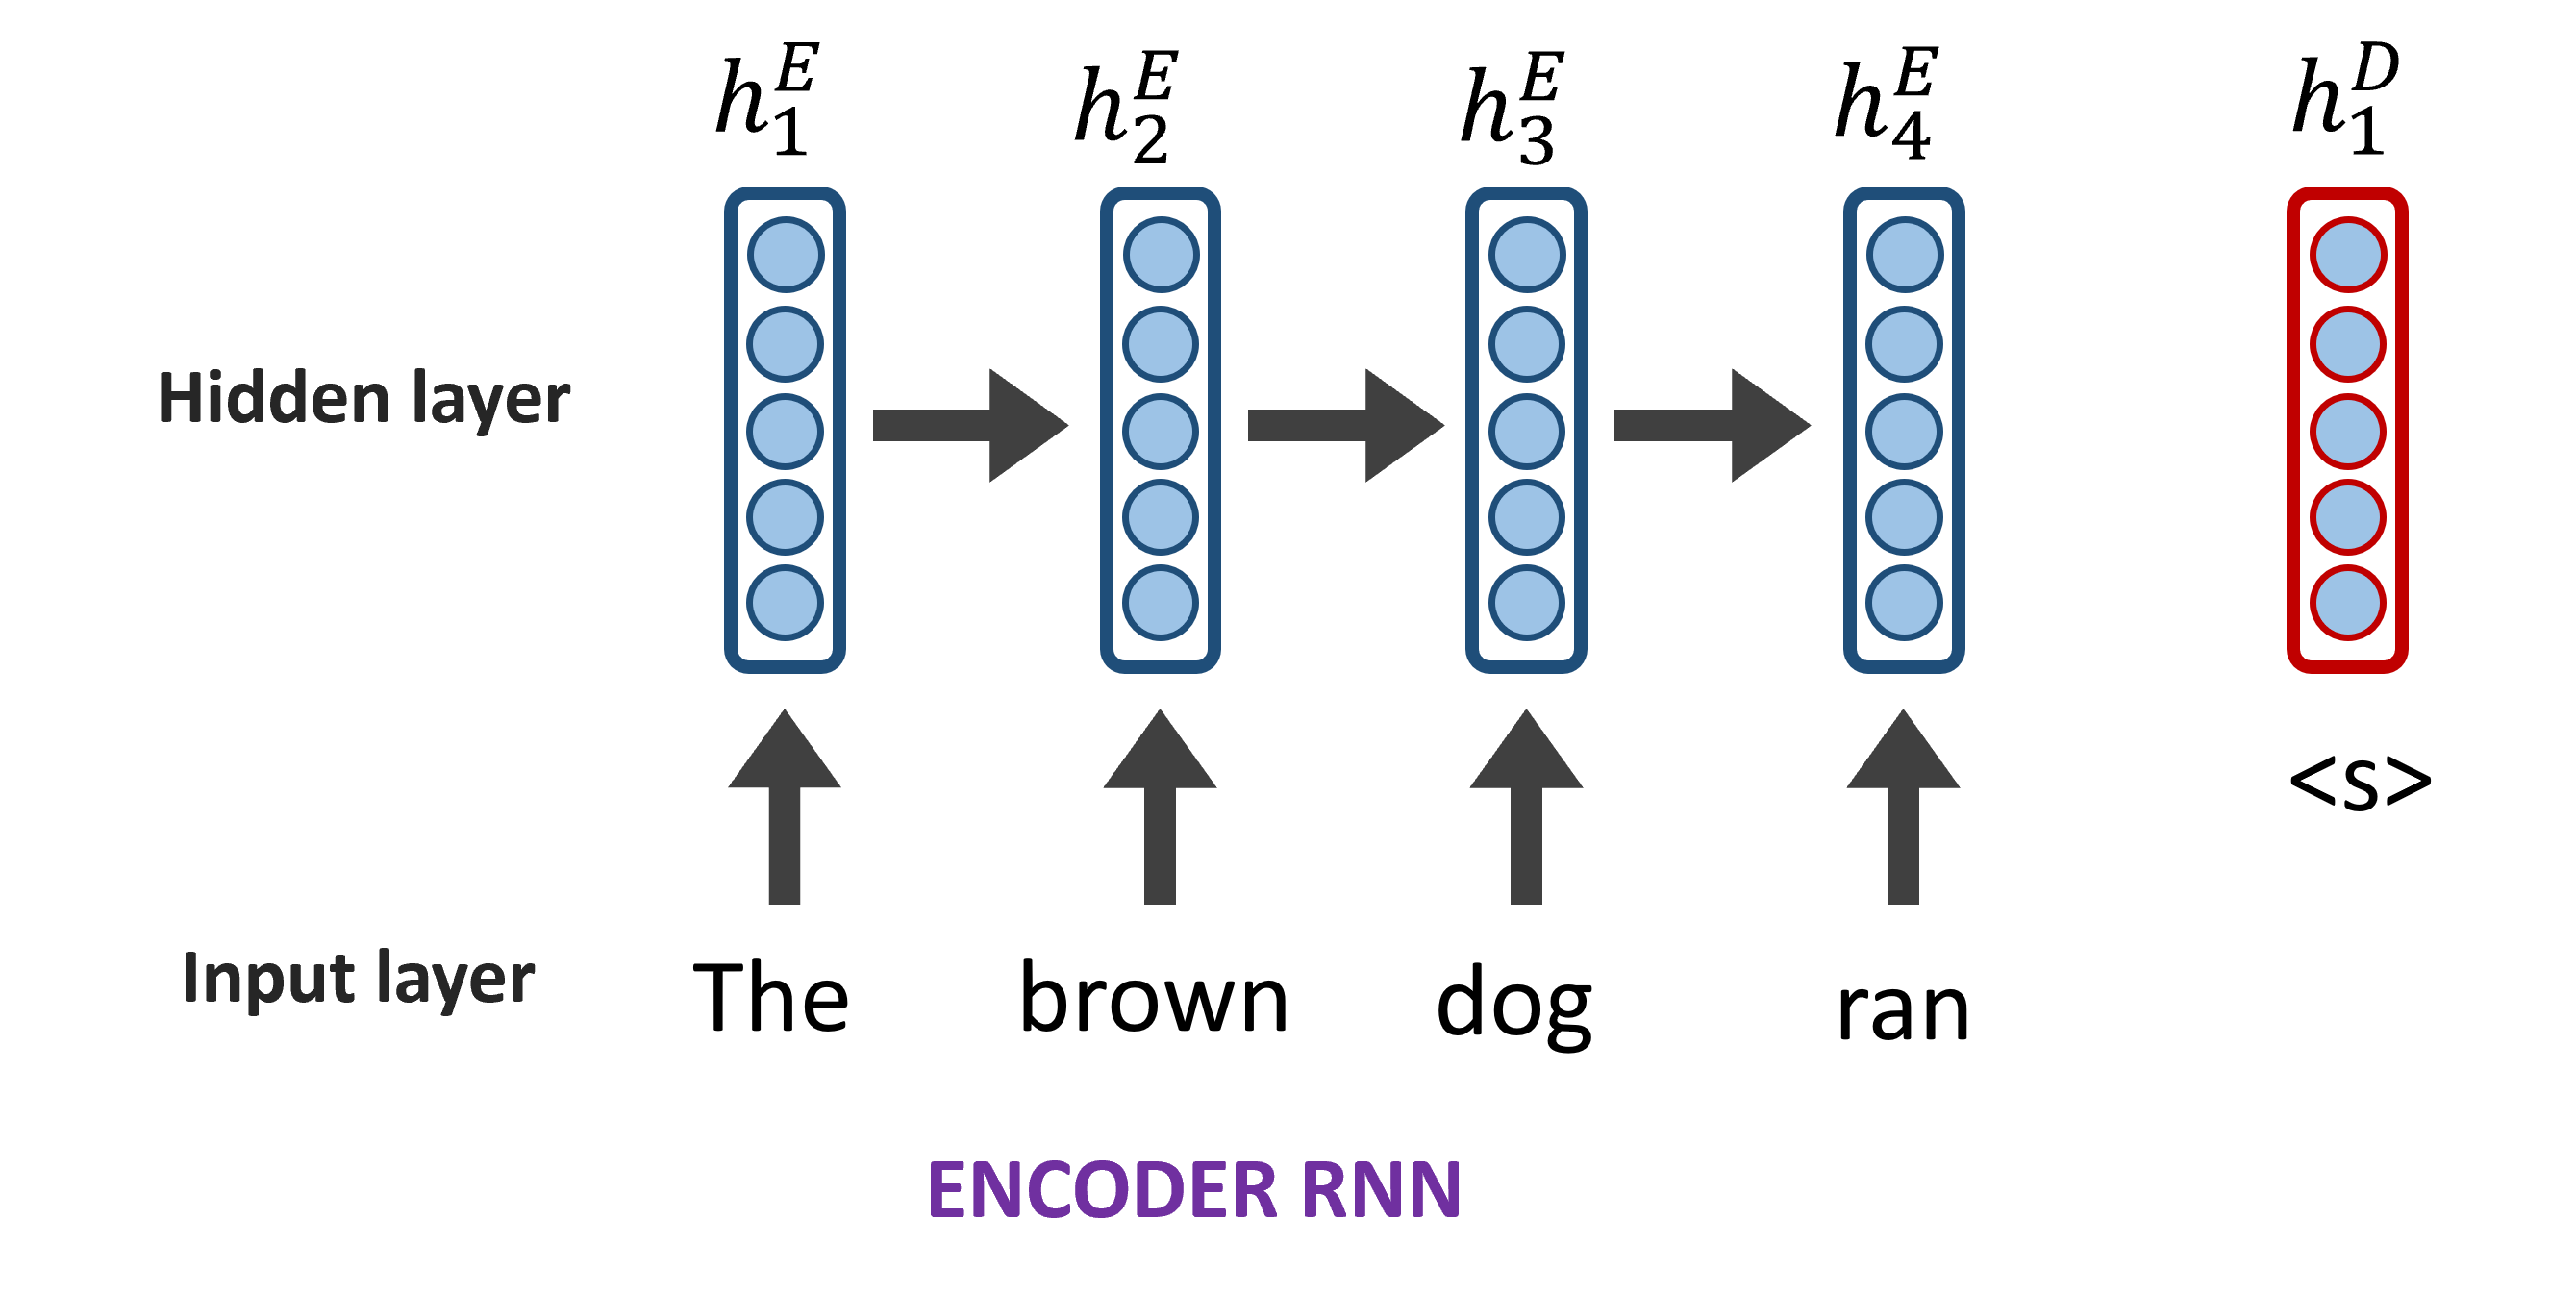
\includegraphics[width=0.8\linewidth,keepaspectratio]{bert17}
% \end{center}	

% \end{frame}

%%%%%%%%%%%%%%%%%%%%%%%%%%%%%%%%%%%%%%%%%%%%%%%%%%%%%%%%%%%
\begin{frame}[fragile]\frametitle{seq2seq + Attention}

Q: How do we determine how much to pay attention to each of the encoder’s hidden layers? 

A: Let’s base it on our decoder’s previous hidden state (our latest representation of meaning) and all of the encoder’s hidden layers! We want to measure similarity between decoder hidden state and encoder hidden states in some ways. 



\begin{center}
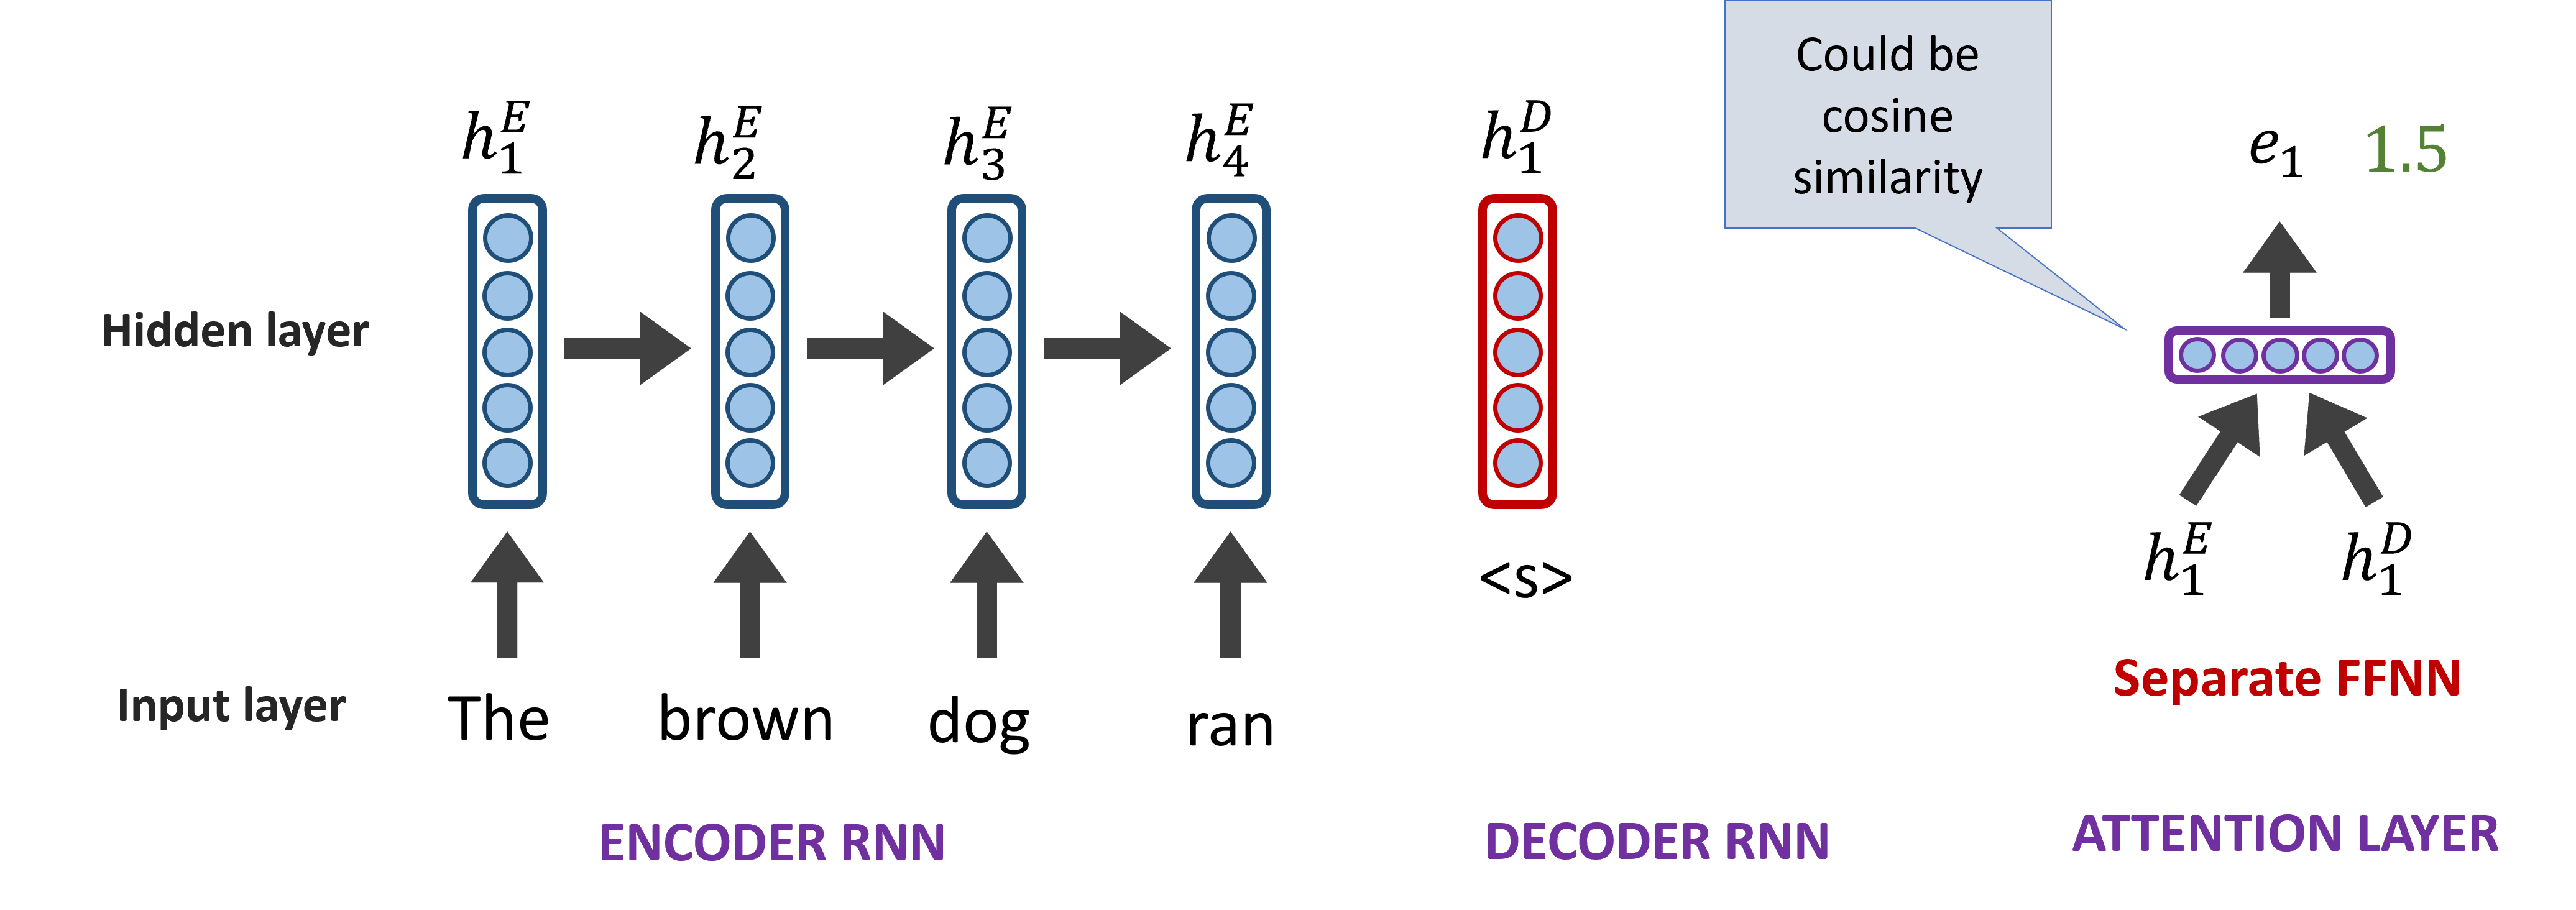
\includegraphics[width=\linewidth,keepaspectratio]{bert18}
\end{center}	

\end{frame}

%%%%%%%%%%%%%%%%%%%%%%%%%%%%%%%%%%%%%%%%%%%%%%%%%%%%%%%%%%%
\begin{frame}[fragile]\frametitle{seq2seq + Attention}

% Q: How do we determine how much to pay attention to each of the encoder’s hidden layers? 

% A: Let’s base it on our decoder’s previous hidden state (our latest representation of meaning) and all of the encoder’s hidden layers! We want to measure similarity between decoder hidden state and encoder hidden stateS in some ways. 



\begin{center}
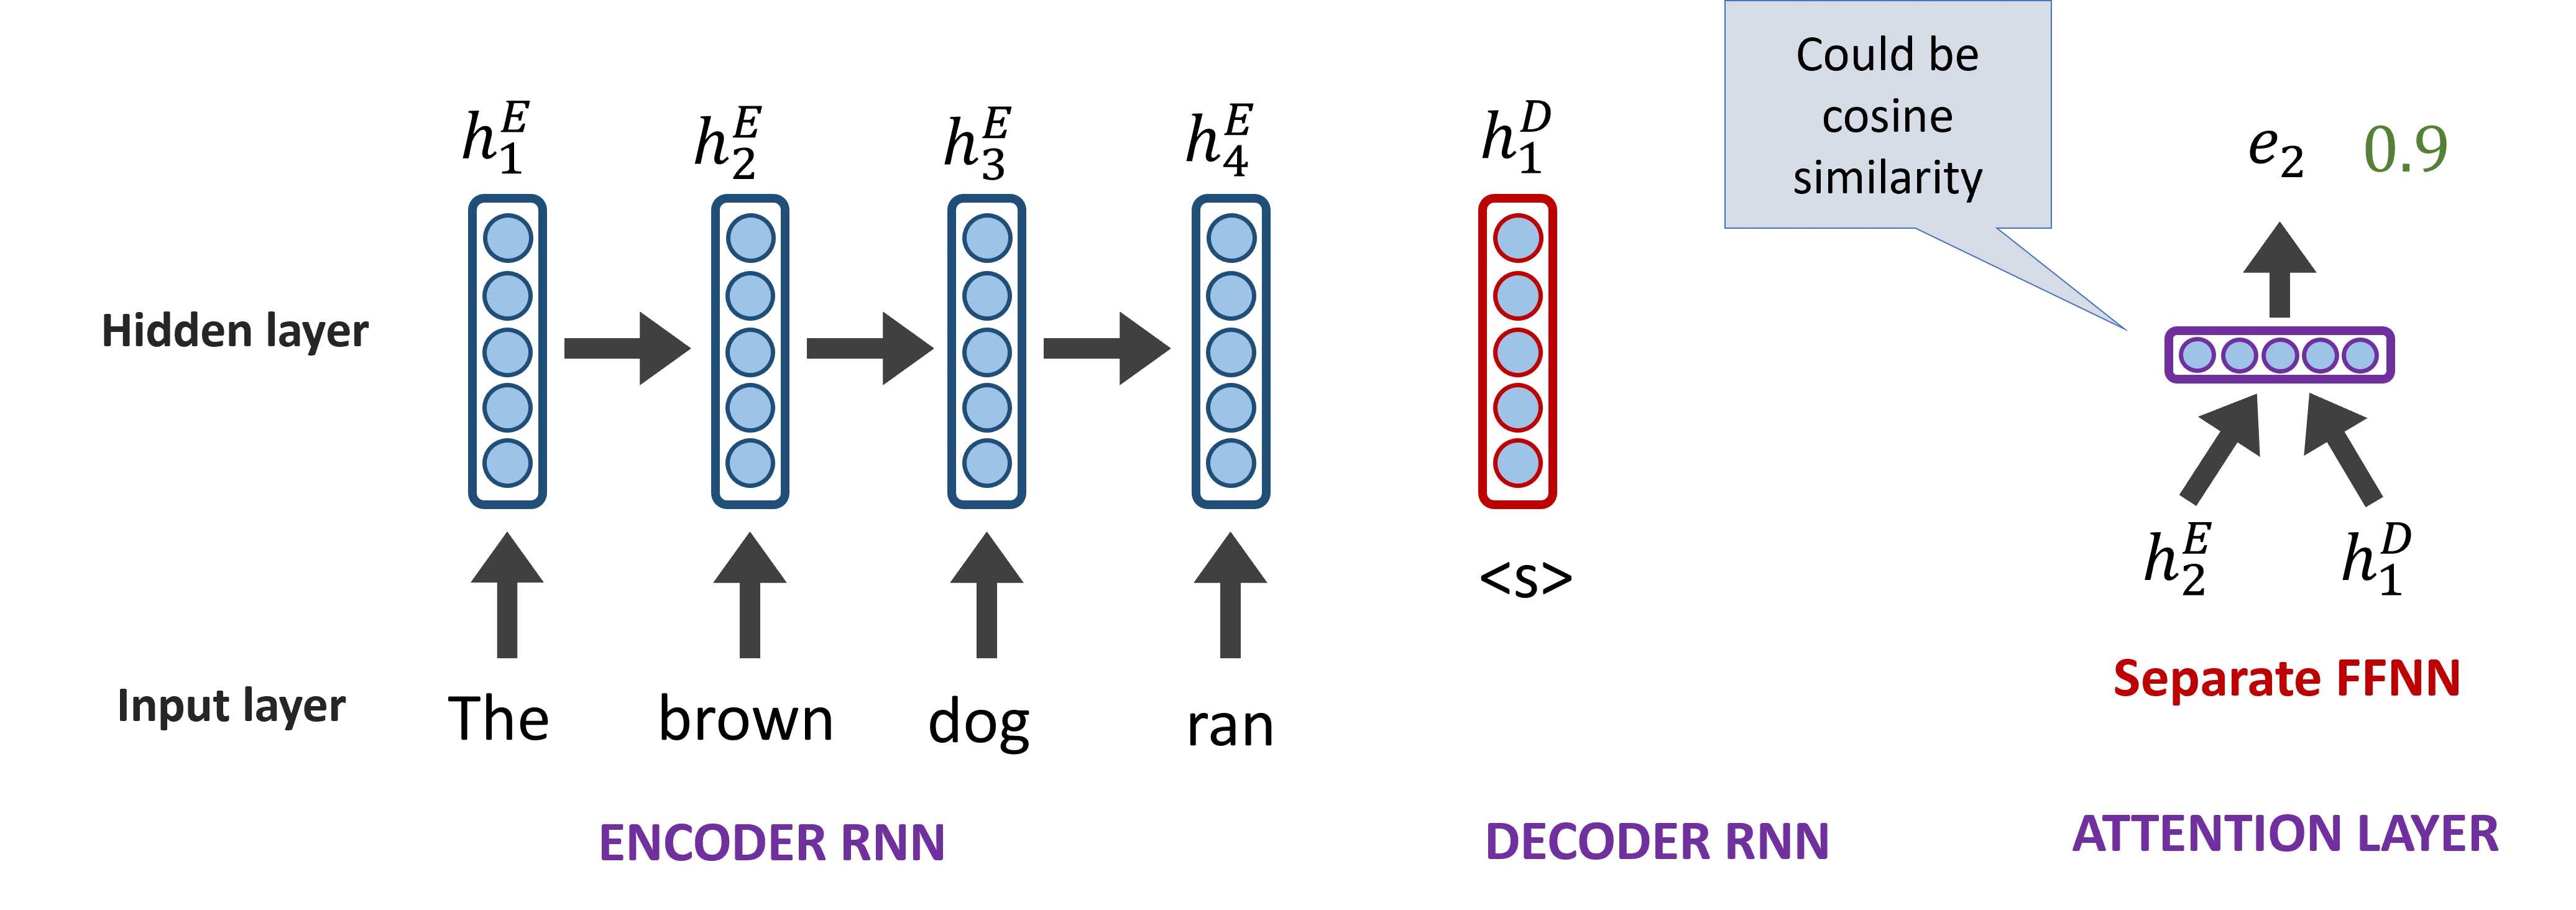
\includegraphics[width=\linewidth,keepaspectratio]{bert19}
\end{center}	

\end{frame}

%%%%%%%%%%%%%%%%%%%%%%%%%%%%%%%%%%%%%%%%%%%%%%%%%%%%%%%%%%%
\begin{frame}[fragile]\frametitle{seq2seq + Attention}

% Q: How do we determine how much to pay attention to each of the encoder’s hidden layers? 

% A: Let’s base it on our decoder’s previous hidden state (our latest representation of meaning) and all of the encoder’s hidden layers! We want to measure similarity between decoder hidden state and encoder hidden stateS in some ways. 



\begin{center}
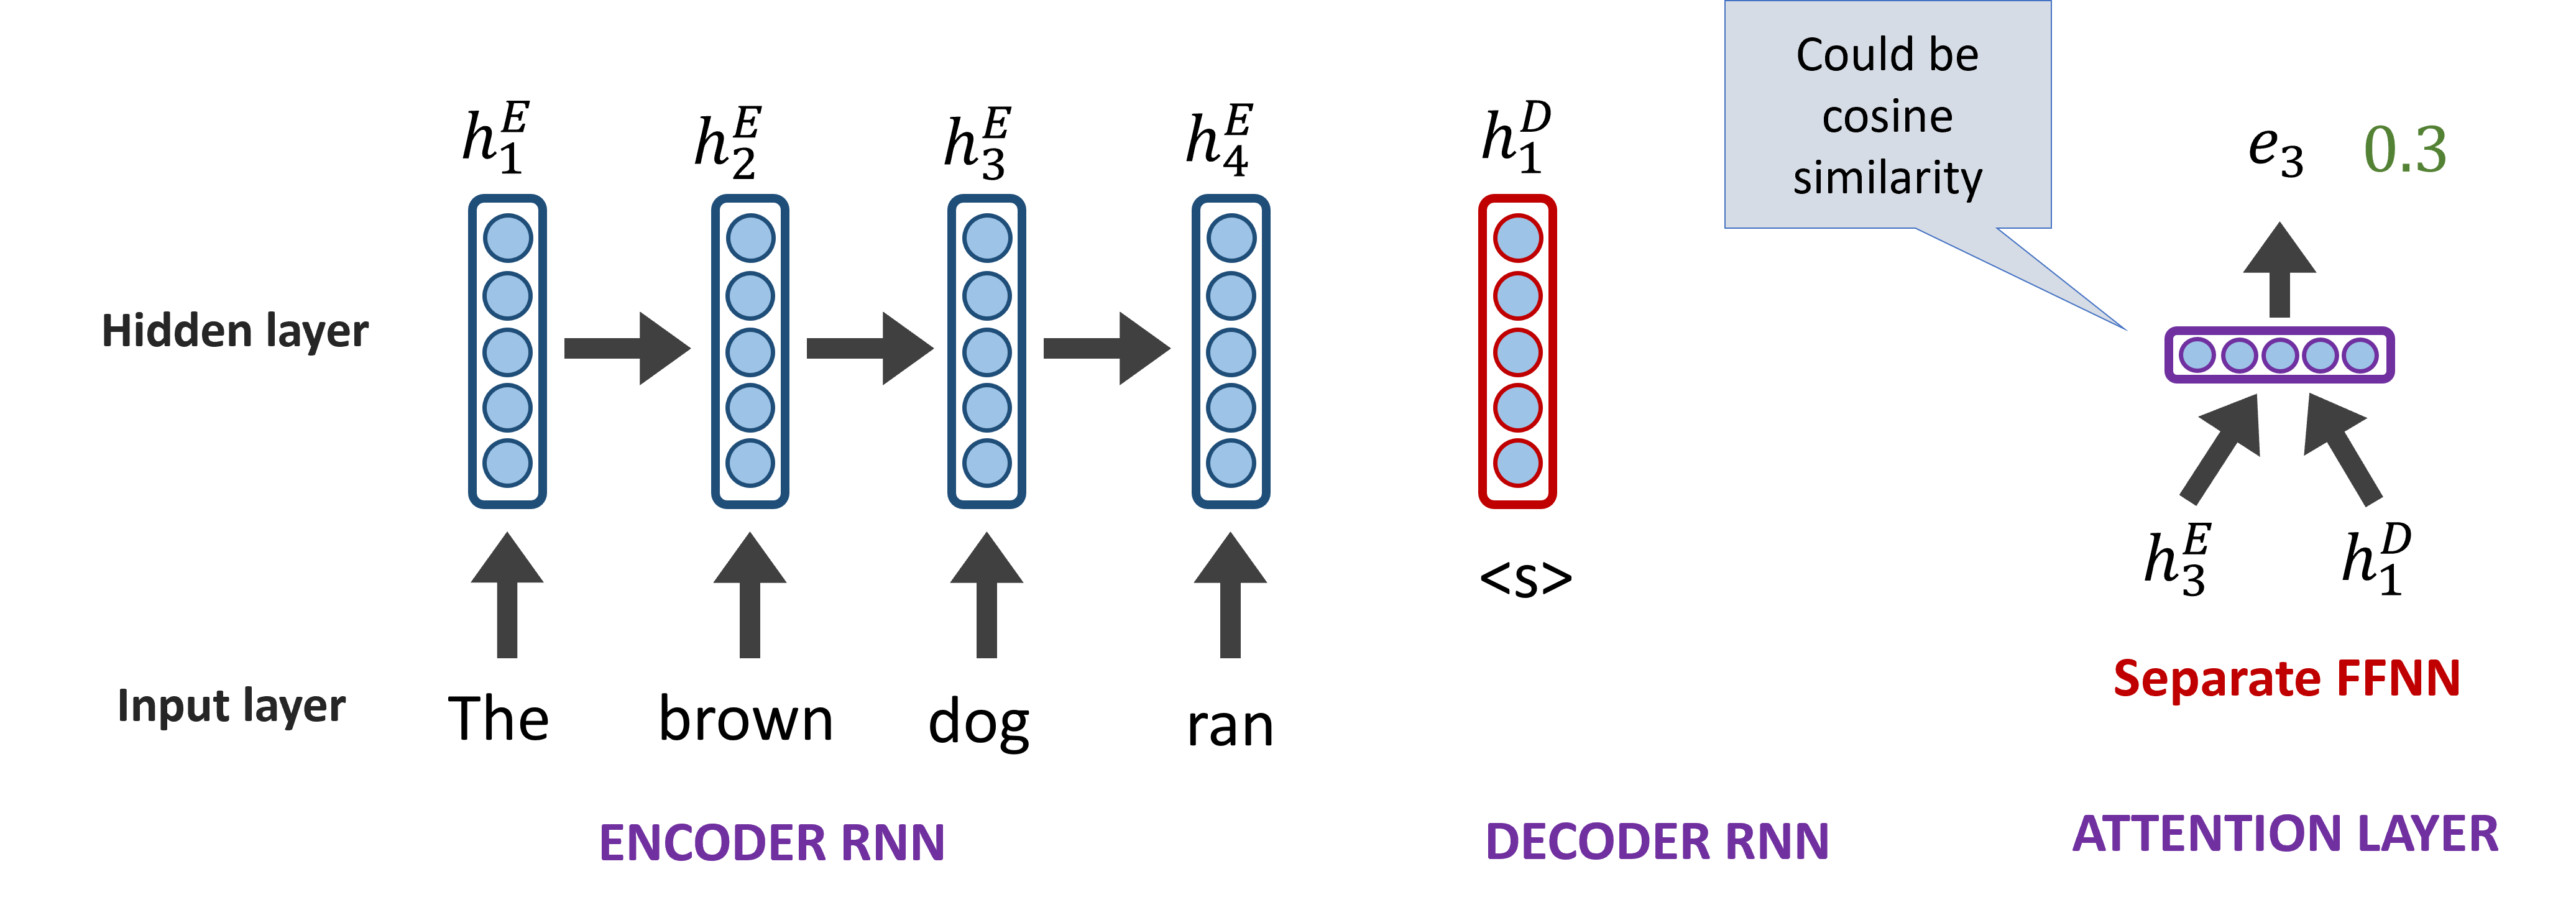
\includegraphics[width=\linewidth,keepaspectratio]{bert20}
\end{center}	

\end{frame}

%%%%%%%%%%%%%%%%%%%%%%%%%%%%%%%%%%%%%%%%%%%%%%%%%%%%%%%%%%%
\begin{frame}[fragile]\frametitle{seq2seq + Attention}

% Q: How do we determine how much to pay attention to each of the encoder’s hidden layers? 

% A: Let’s base it on our decoder’s previous hidden state (our latest representation of meaning) and all of the encoder’s hidden layers! We want to measure similarity between decoder hidden state and encoder hidden stateS in some ways. 



\begin{center}
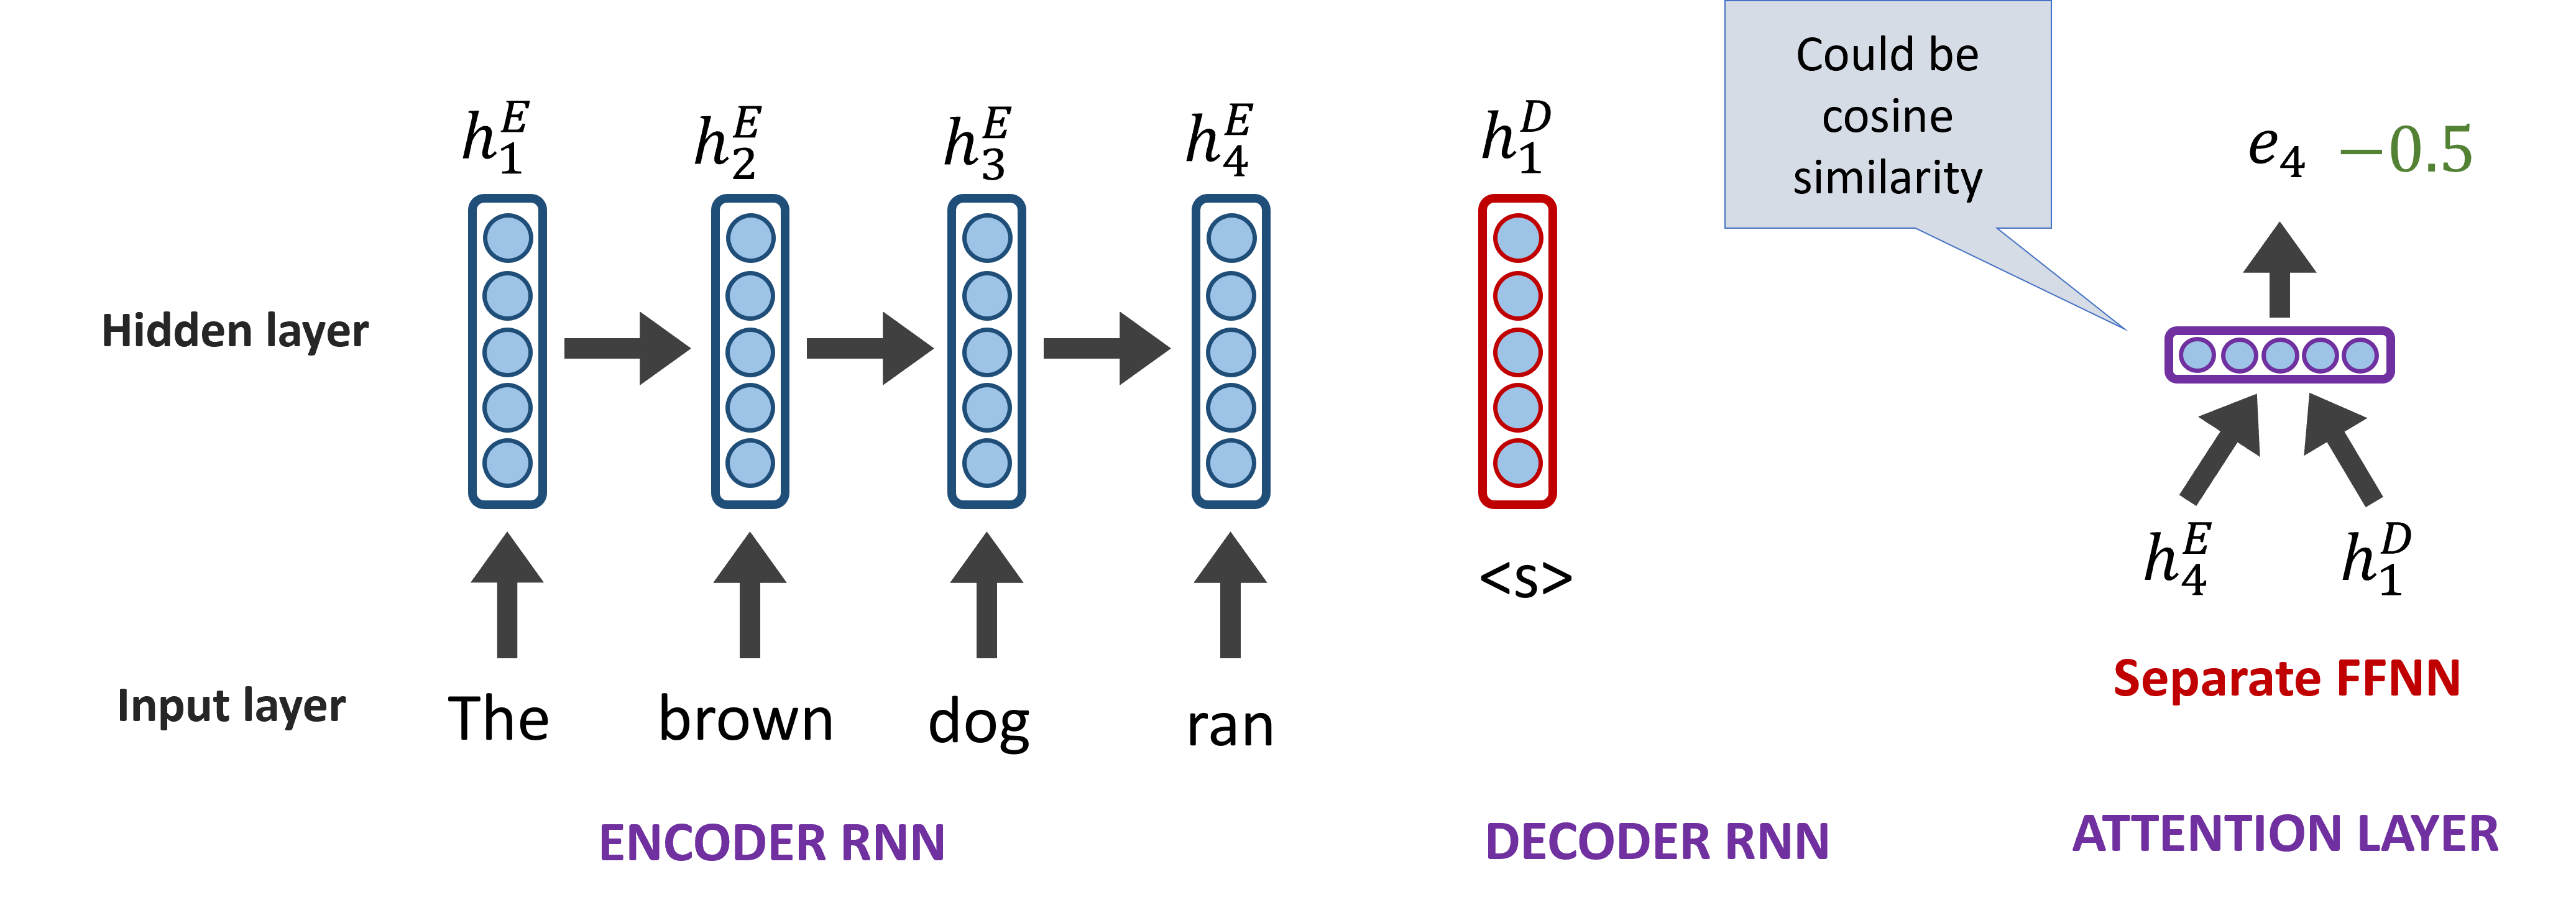
\includegraphics[width=\linewidth,keepaspectratio]{bert21}
\end{center}	

\end{frame}

%%%%%%%%%%%%%%%%%%%%%%%%%%%%%%%%%%%%%%%%%%%%%%%%%%%%%%%%%%%
\begin{frame}[fragile]\frametitle{seq2seq + Attention}

% Q: How do we determine how much to pay attention to each of the encoder’s hidden layers? 

% A: Let’s base it on our decoder’s previous hidden state (our latest representation of meaning) and all of the encoder’s hidden layers!



\begin{center}
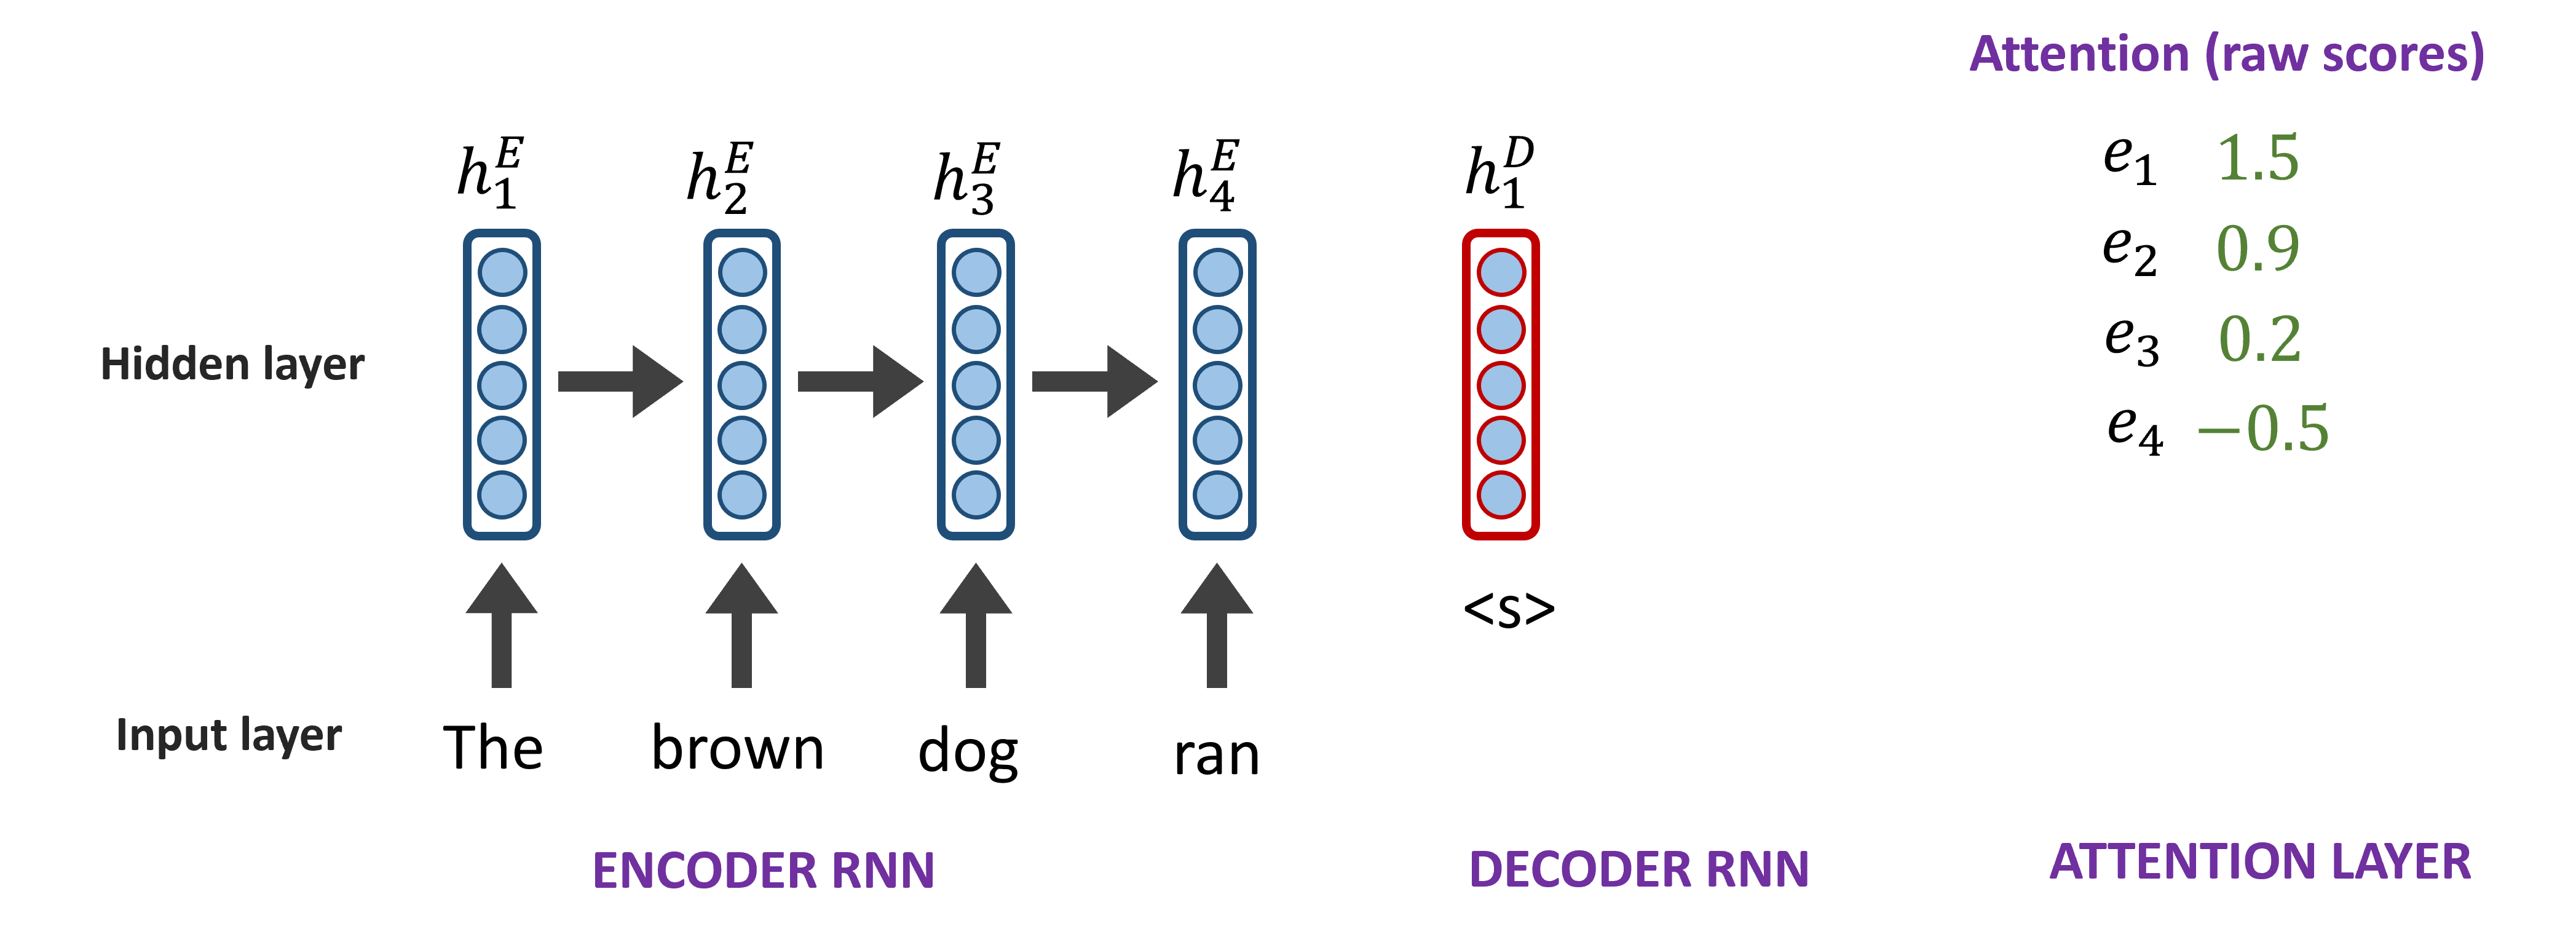
\includegraphics[width=\linewidth,keepaspectratio]{bert22}
\end{center}	

\end{frame}

%%%%%%%%%%%%%%%%%%%%%%%%%%%%%%%%%%%%%%%%%%%%%%%%%%%%%%%%%%%
\begin{frame}[fragile]\frametitle{seq2seq + Attention}

% Q: How do we determine how much to pay attention to each of the encoder’s hidden layers? 

% A: Let’s base it on our decoder’s previous hidden state (our latest representation of meaning) and all of the encoder’s hidden layers!



\begin{center}
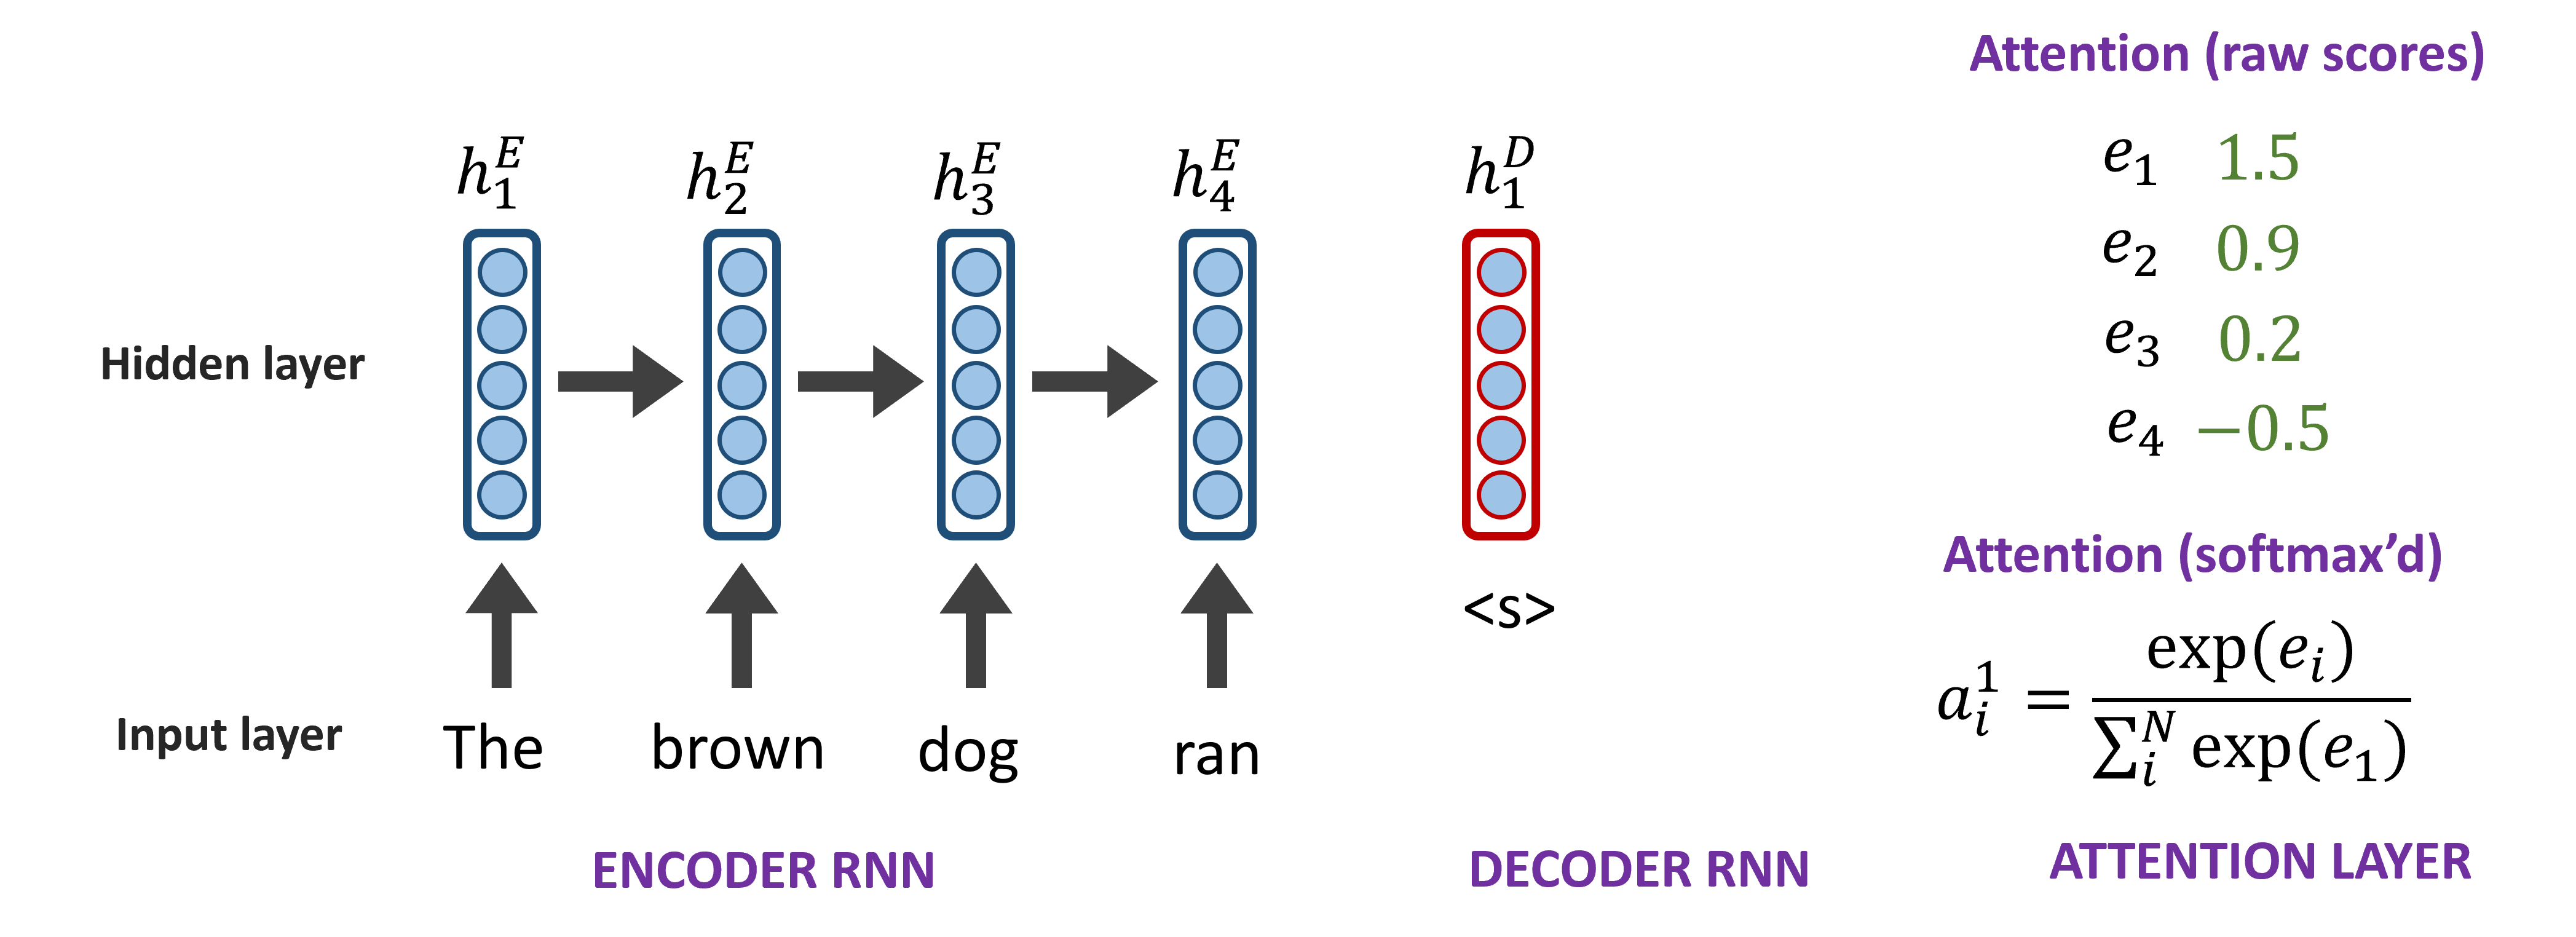
\includegraphics[width=\linewidth,keepaspectratio]{bert23}
\end{center}	

\end{frame}

%%%%%%%%%%%%%%%%%%%%%%%%%%%%%%%%%%%%%%%%%%%%%%%%%%%%%%%%%%%
\begin{frame}[fragile]\frametitle{seq2seq + Attention}

% Q: How do we determine how much to pay attention to each of the encoder’s hidden layers? 

% A: Let’s base it on our decoder’s previous hidden state (our latest representation of meaning) and all of the encoder’s hidden layers!



\begin{center}
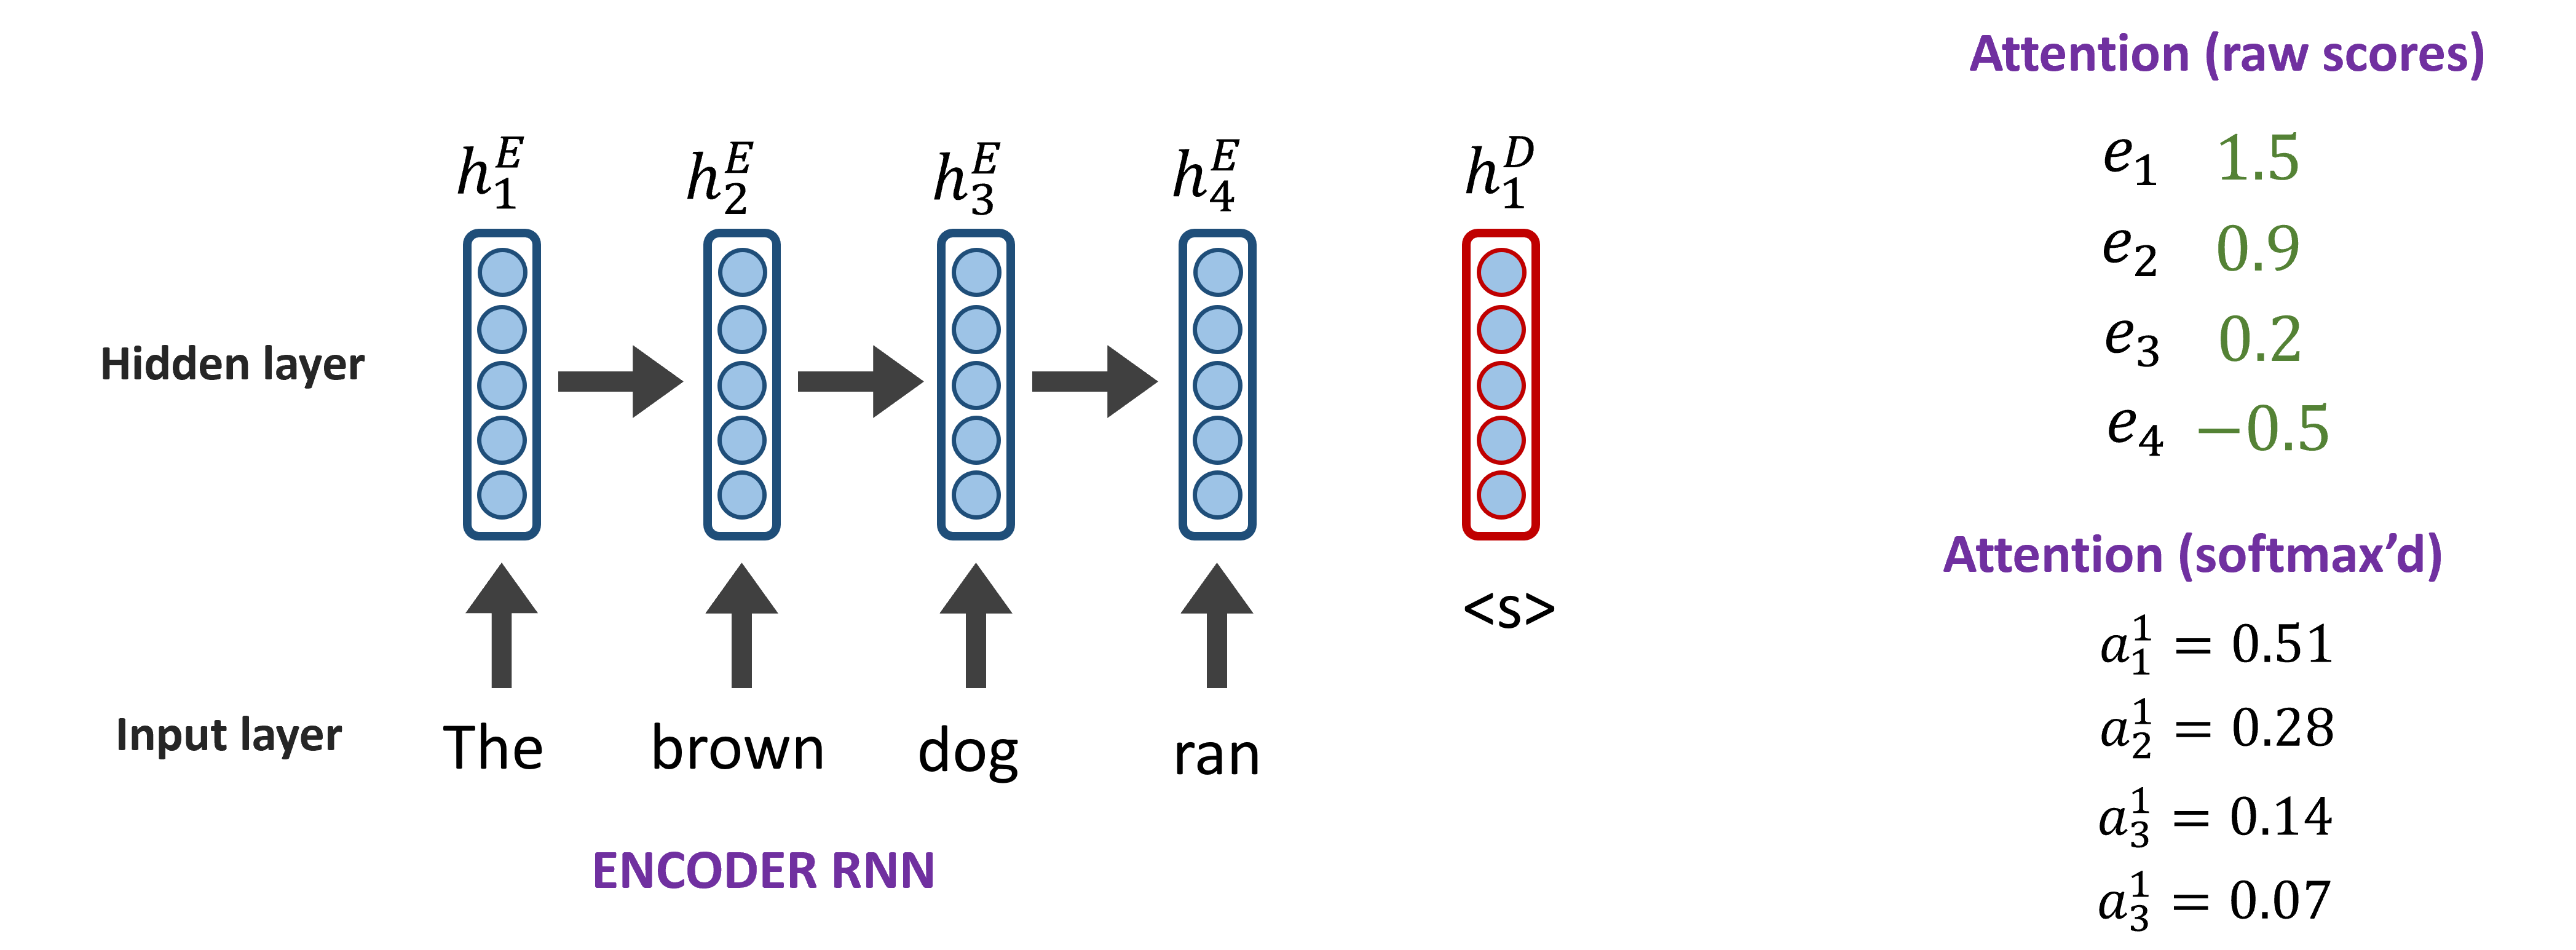
\includegraphics[width=\linewidth,keepaspectratio]{bert24}
\end{center}	

\end{frame}

%%%%%%%%%%%%%%%%%%%%%%%%%%%%%%%%%%%%%%%%%%%%%%%%%%%%%%%%%%%
\begin{frame}[fragile]\frametitle{seq2seq + Attention}

\begin{center}
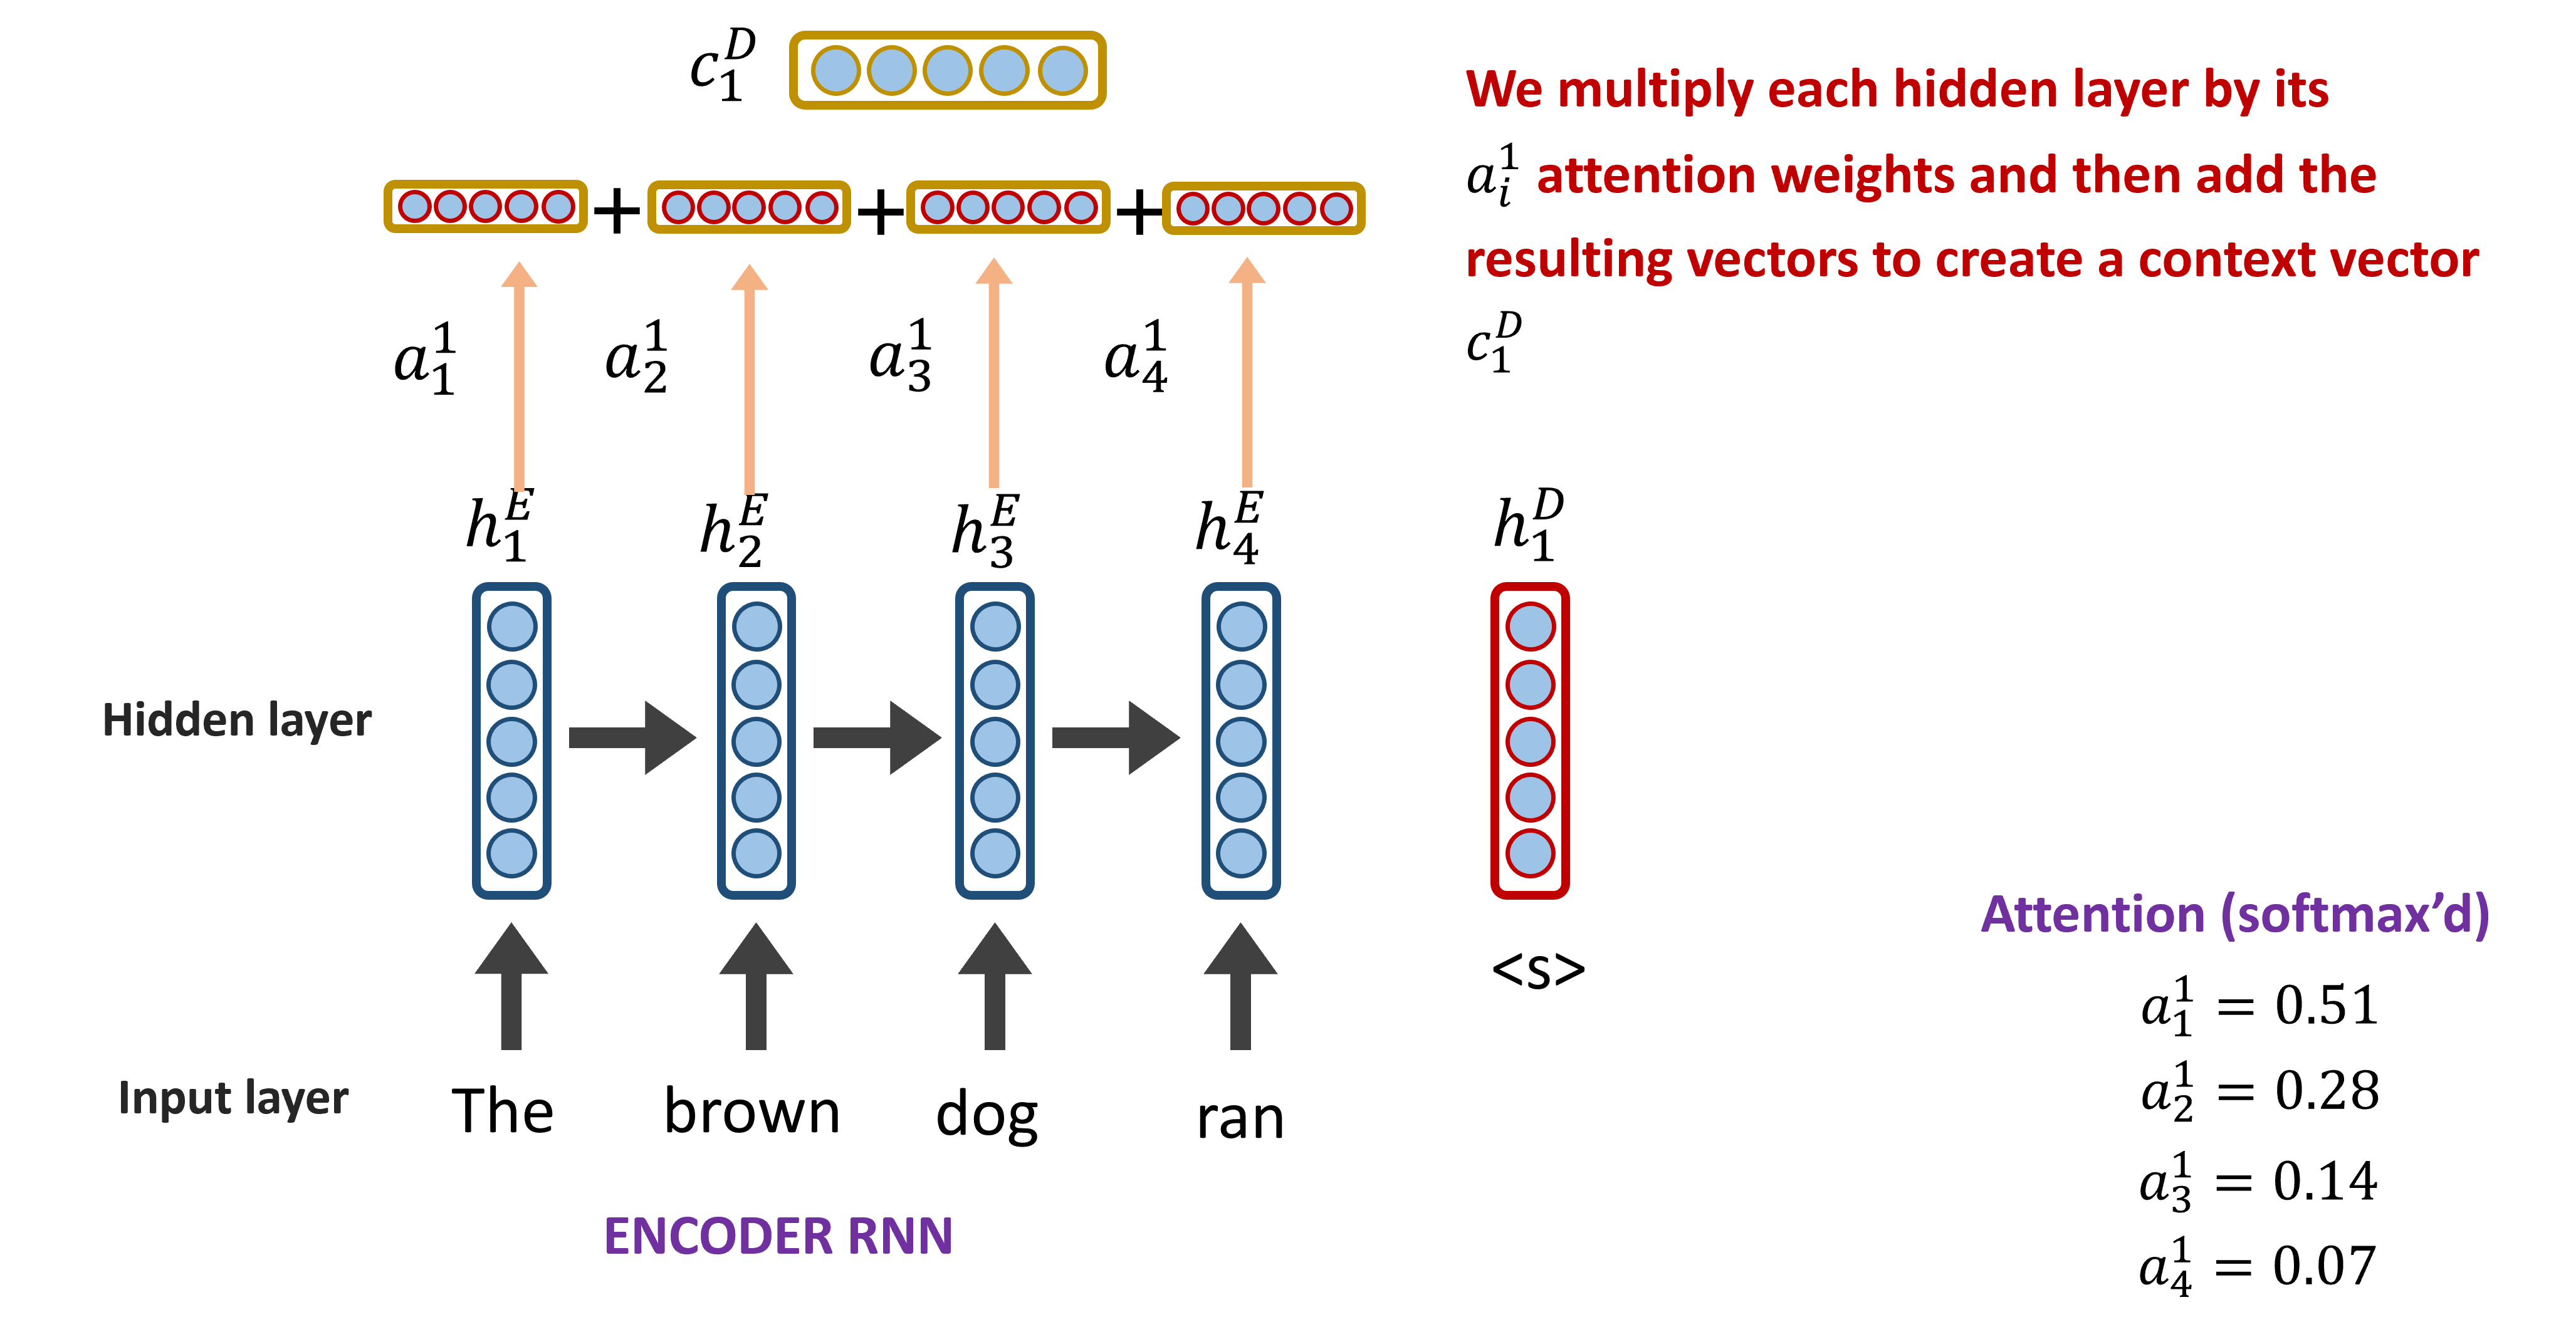
\includegraphics[width=\linewidth,keepaspectratio]{bert25}
\end{center}	

\end{frame}

% %%%%%%%%%%%%%%%%%%%%%%%%%%%%%%%%%%%%%%%%%%%%%%%%%%%%%%%%%%%
% \begin{frame}[fragile]\frametitle{seq2seq + Attention}

% \begin{center}
% 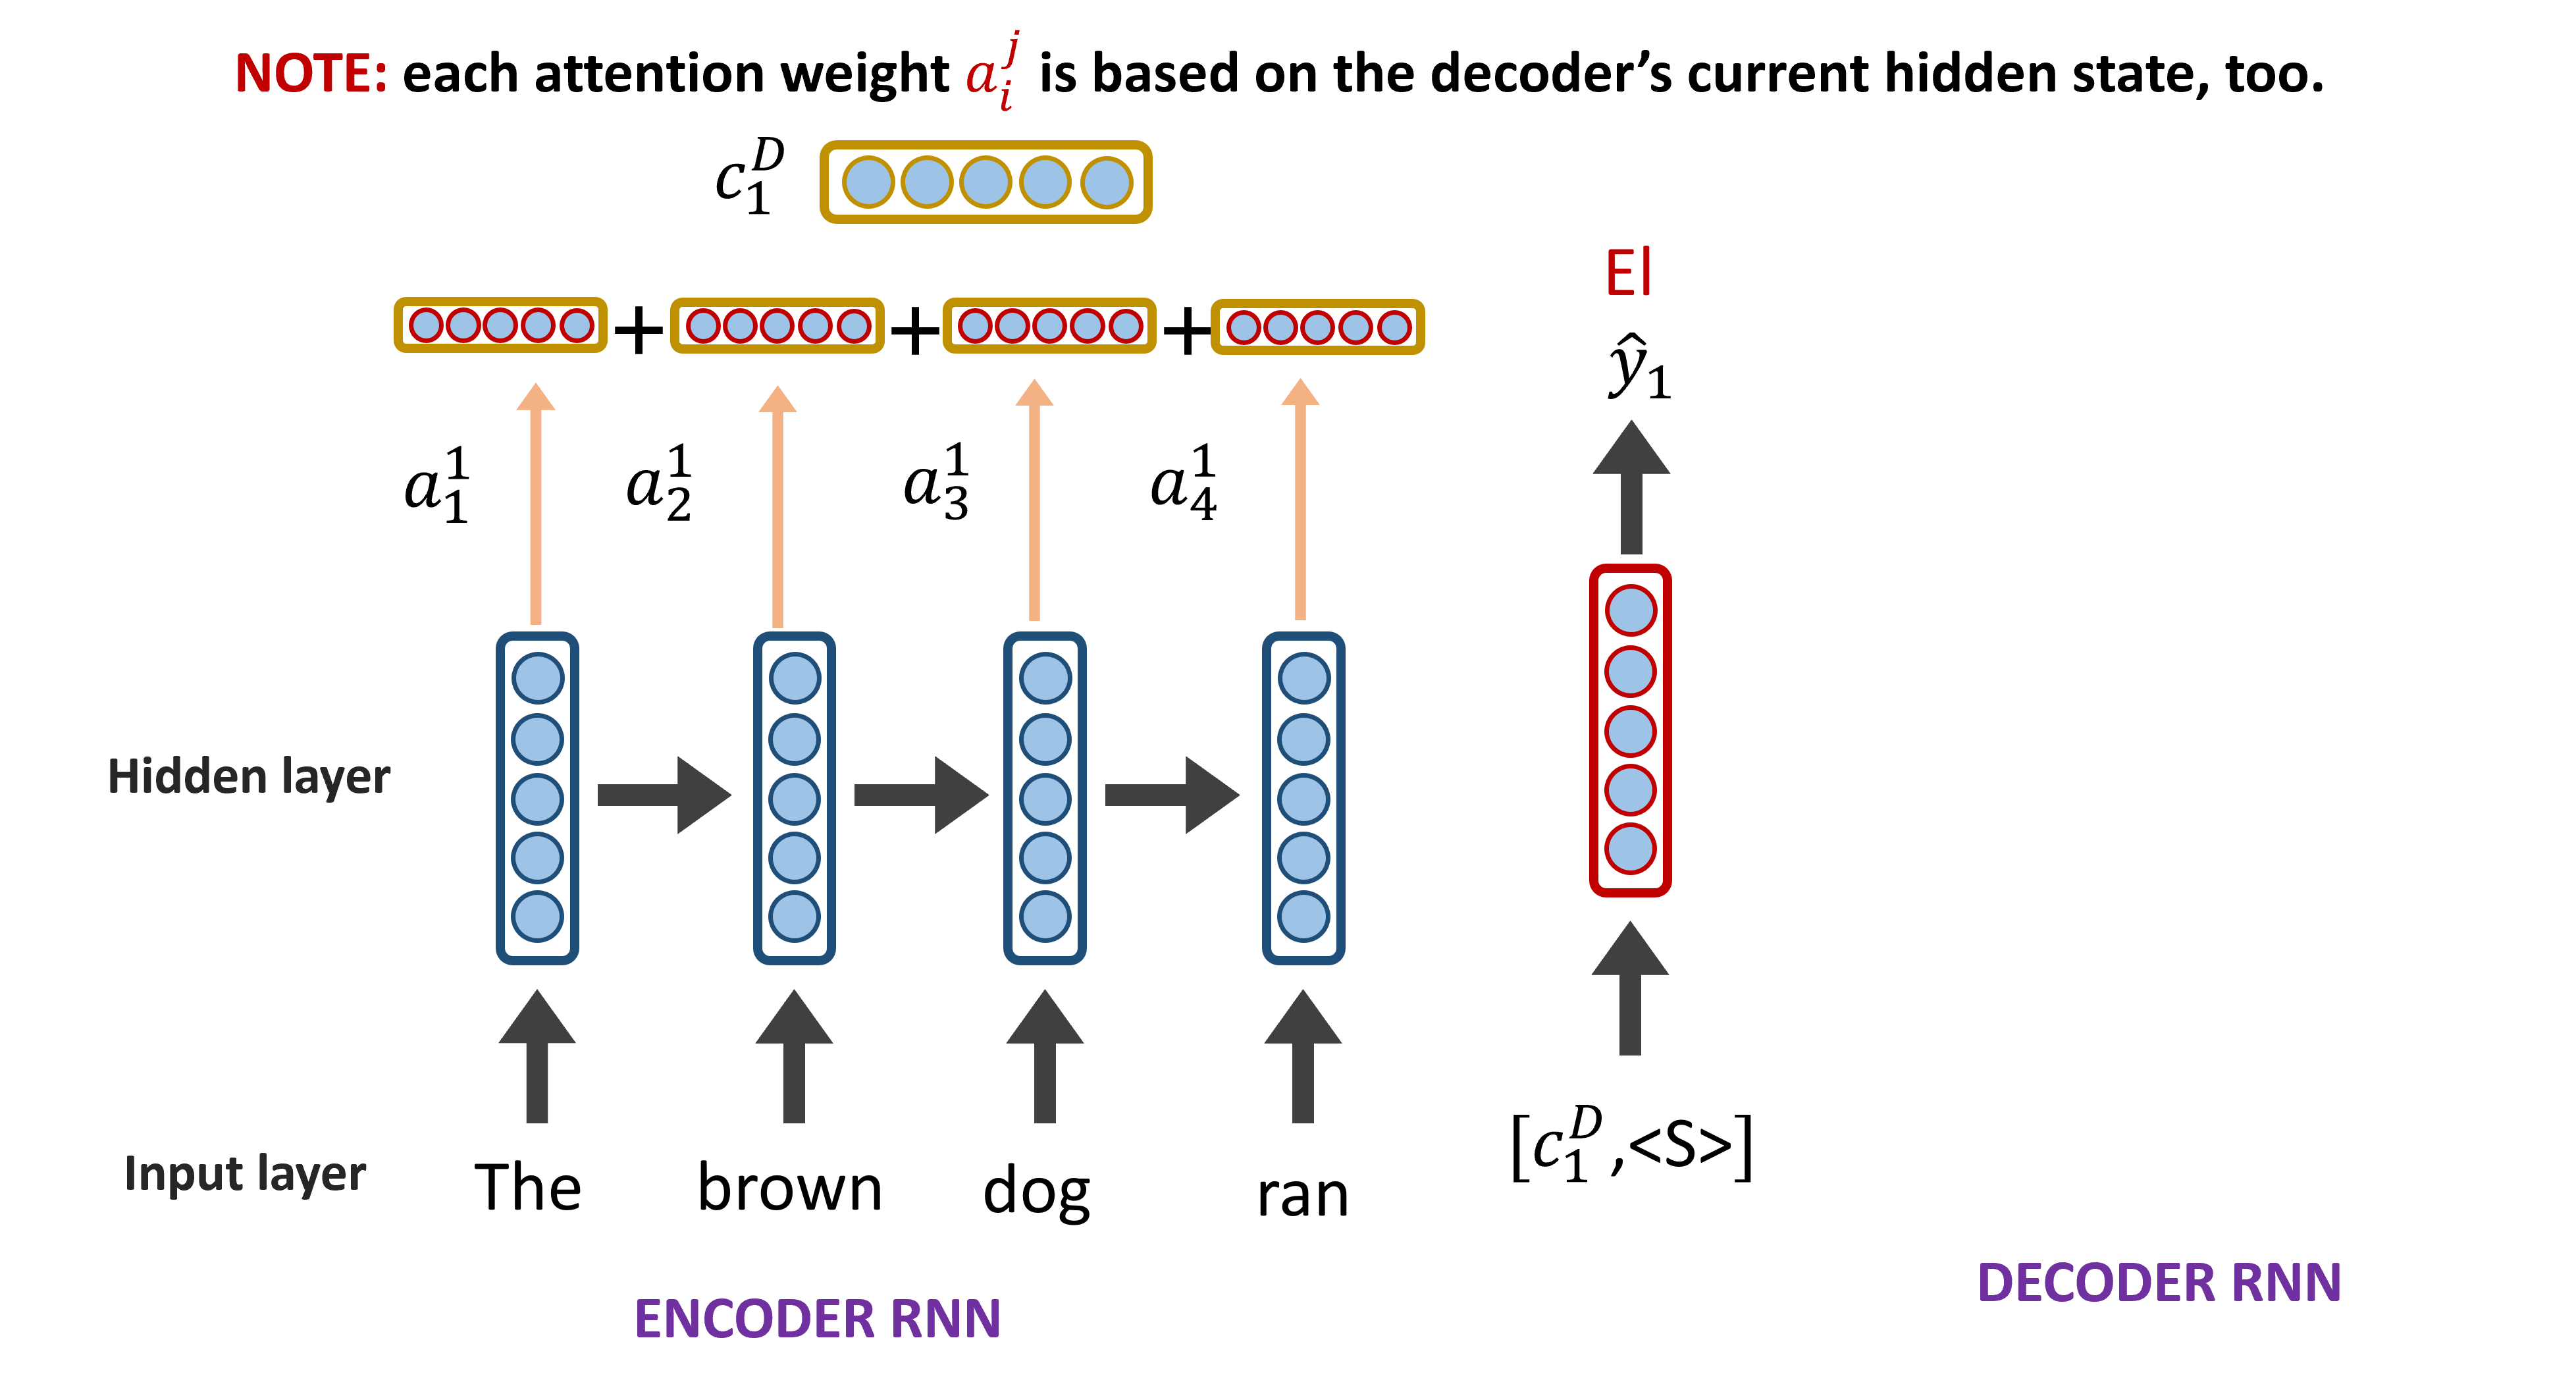
\includegraphics[width=\linewidth,keepaspectratio]{bert26}
% \end{center}	

% \end{frame}

% %%%%%%%%%%%%%%%%%%%%%%%%%%%%%%%%%%%%%%%%%%%%%%%%%%%%%%%%%%%
% \begin{frame}[fragile]\frametitle{seq2seq + Attention}

% \begin{center}
% 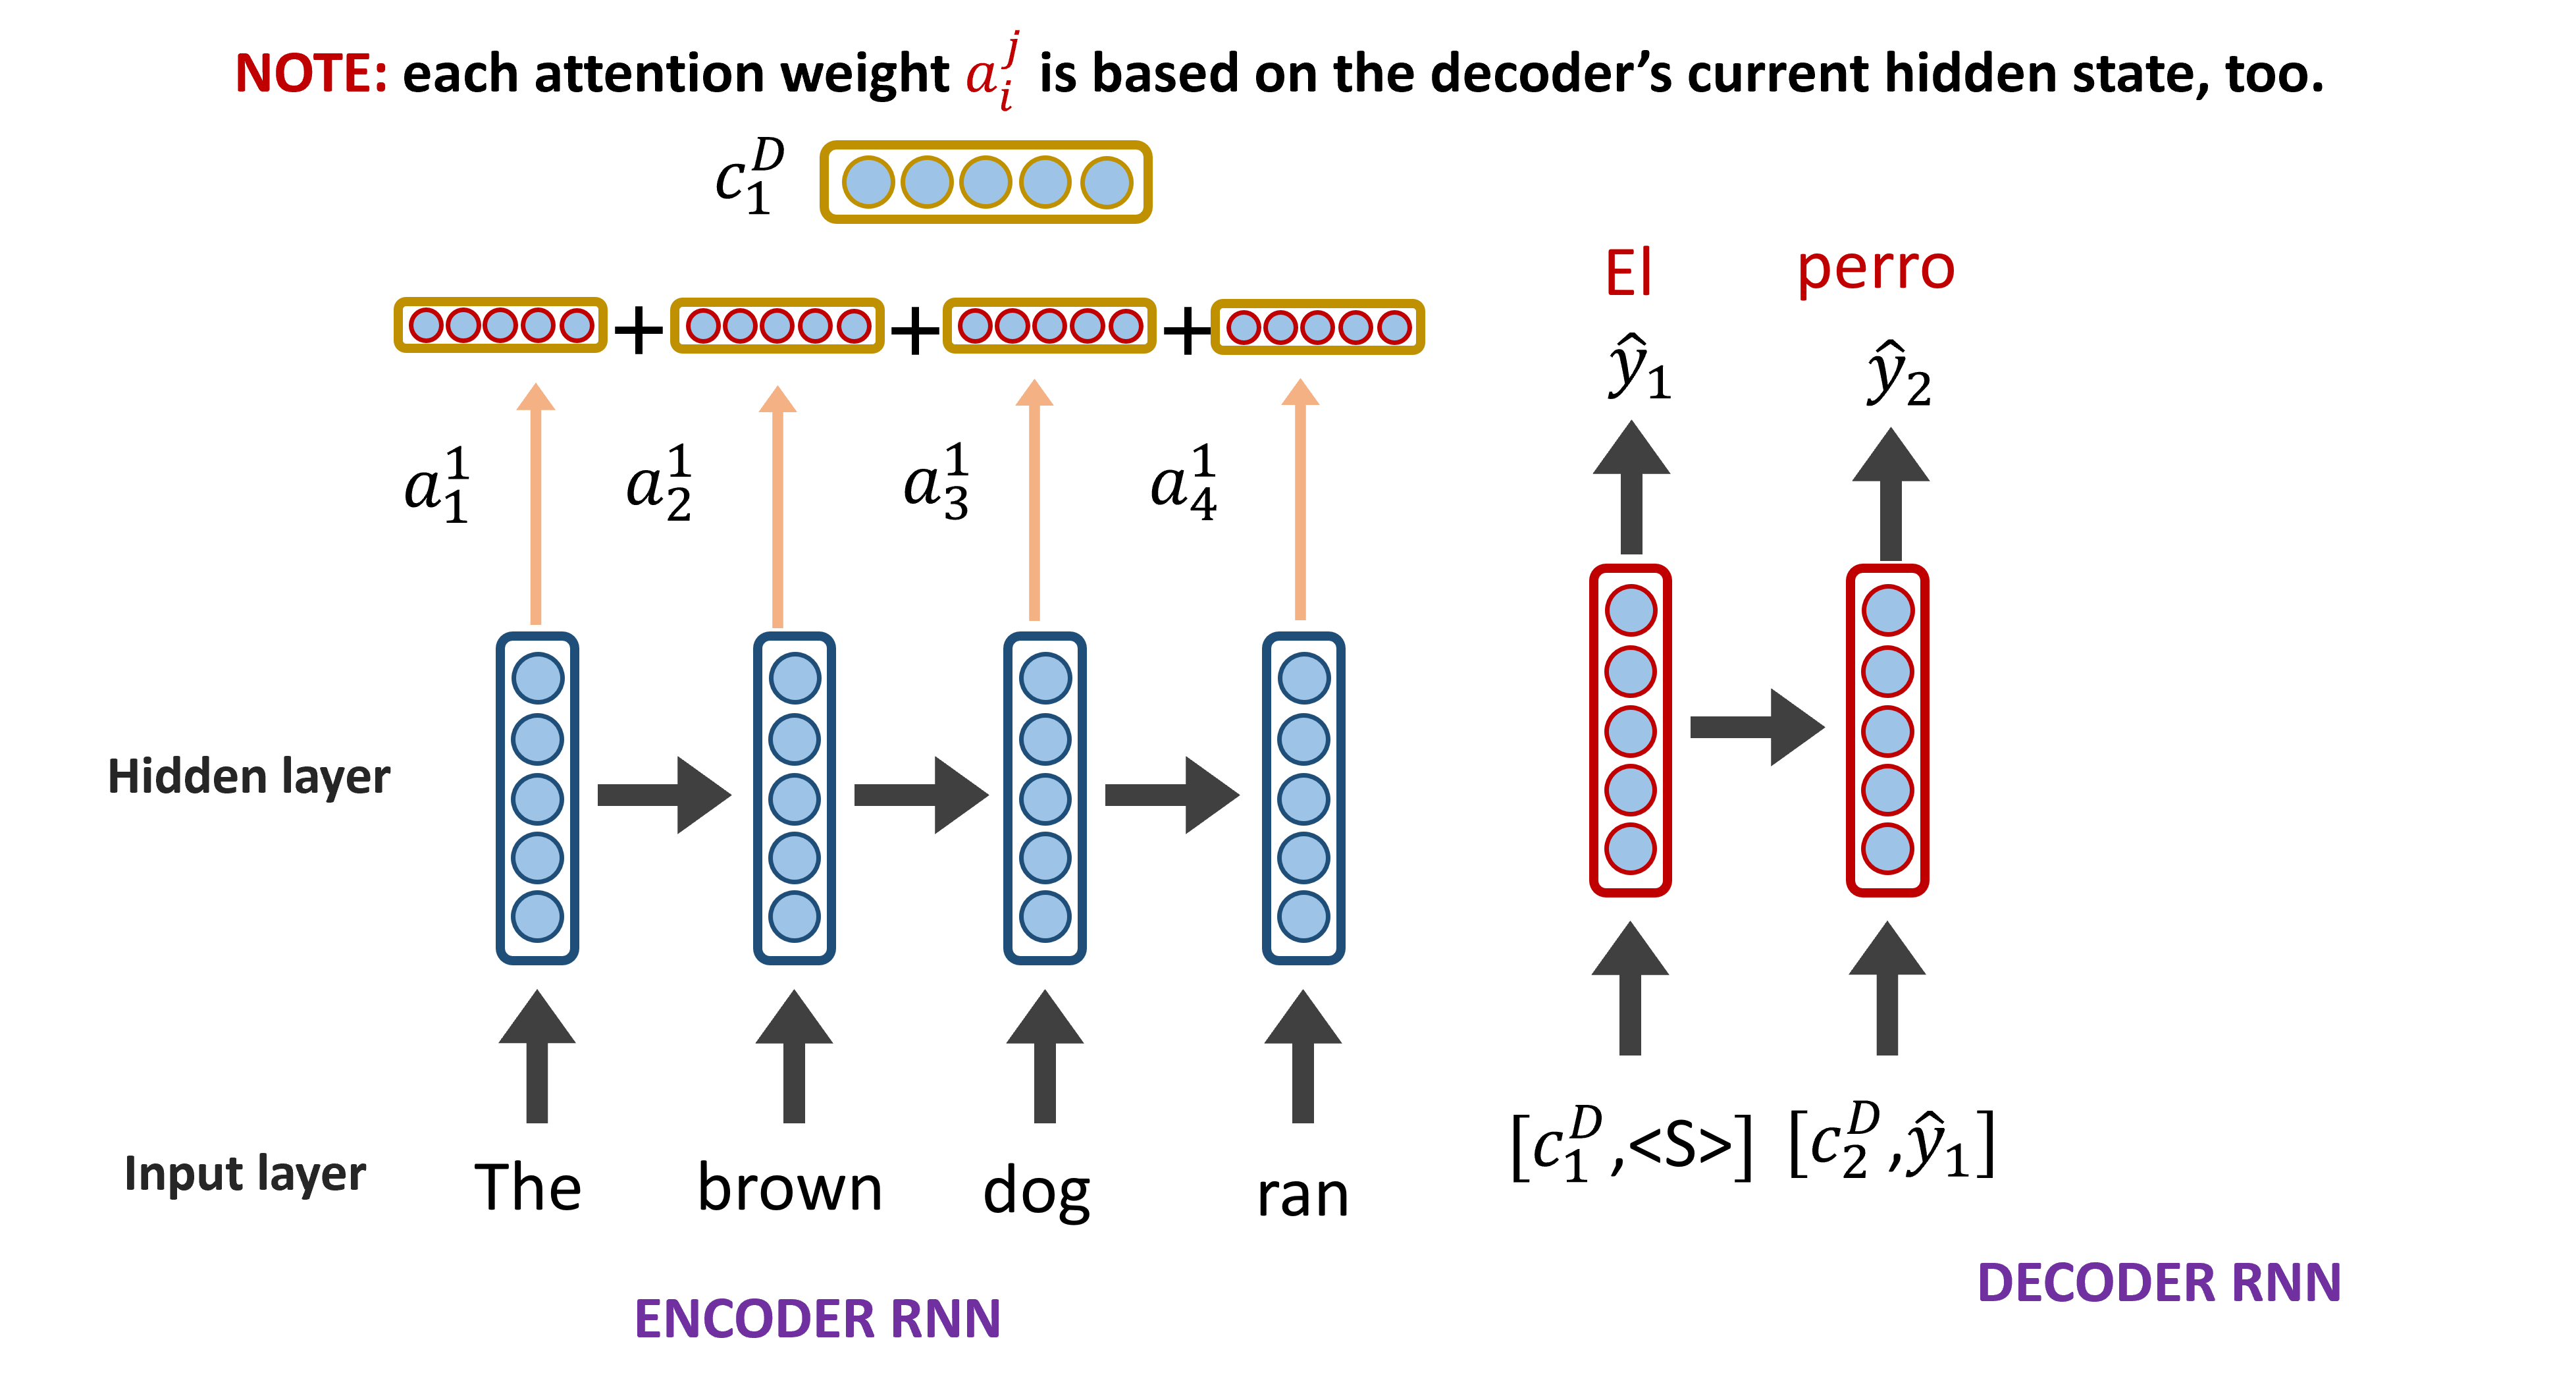
\includegraphics[width=\linewidth,keepaspectratio]{bert27}
% \end{center}	

% \end{frame}


%%%%%%%%%%%%%%%%%%%%%%%%%%%%%%%%%%%%%%%%%%%%%%%%%%%%%%%%%%%
\begin{frame}[fragile]\frametitle{seq2seq + Attention}

\begin{center}
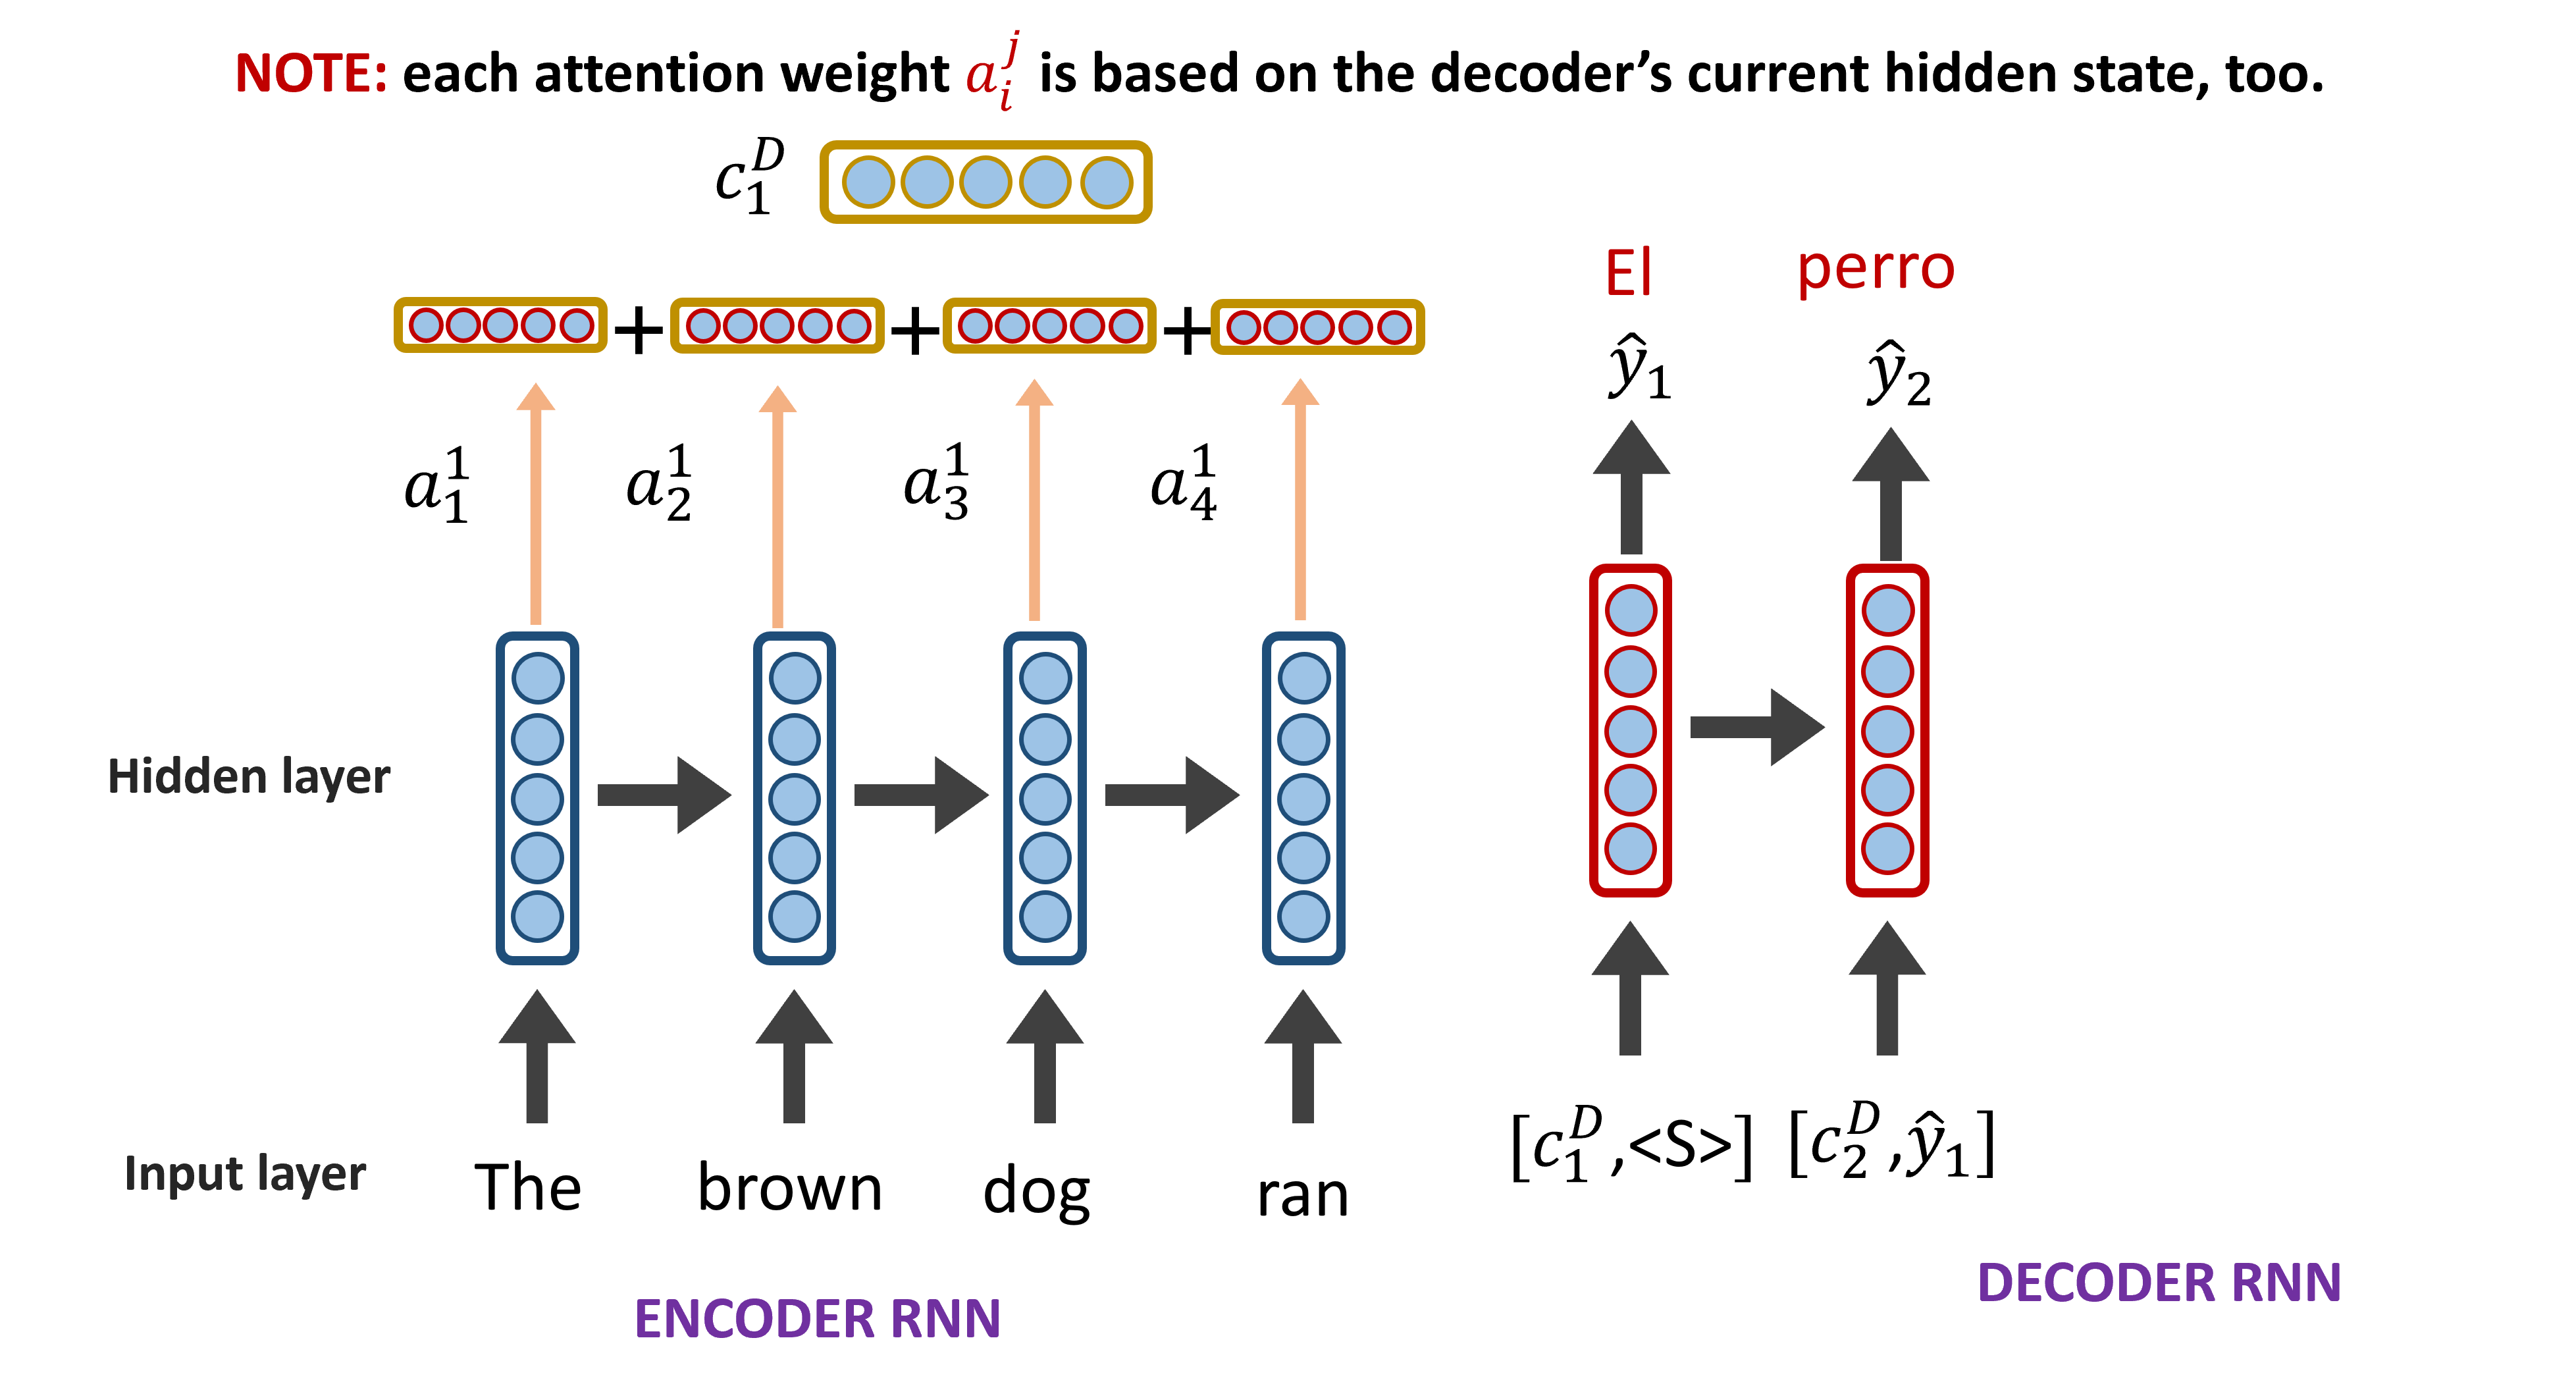
\includegraphics[width=\linewidth,keepaspectratio]{bert28}
\end{center}	

\end{frame}

%%%%%%%%%%%%%%%%%%%%%%%%%%%%%%%%%%%%%%%%%%%%%%%%%%%%%%%%%%%
\begin{frame}[fragile]\frametitle{seq2seq + Attention}

\begin{center}
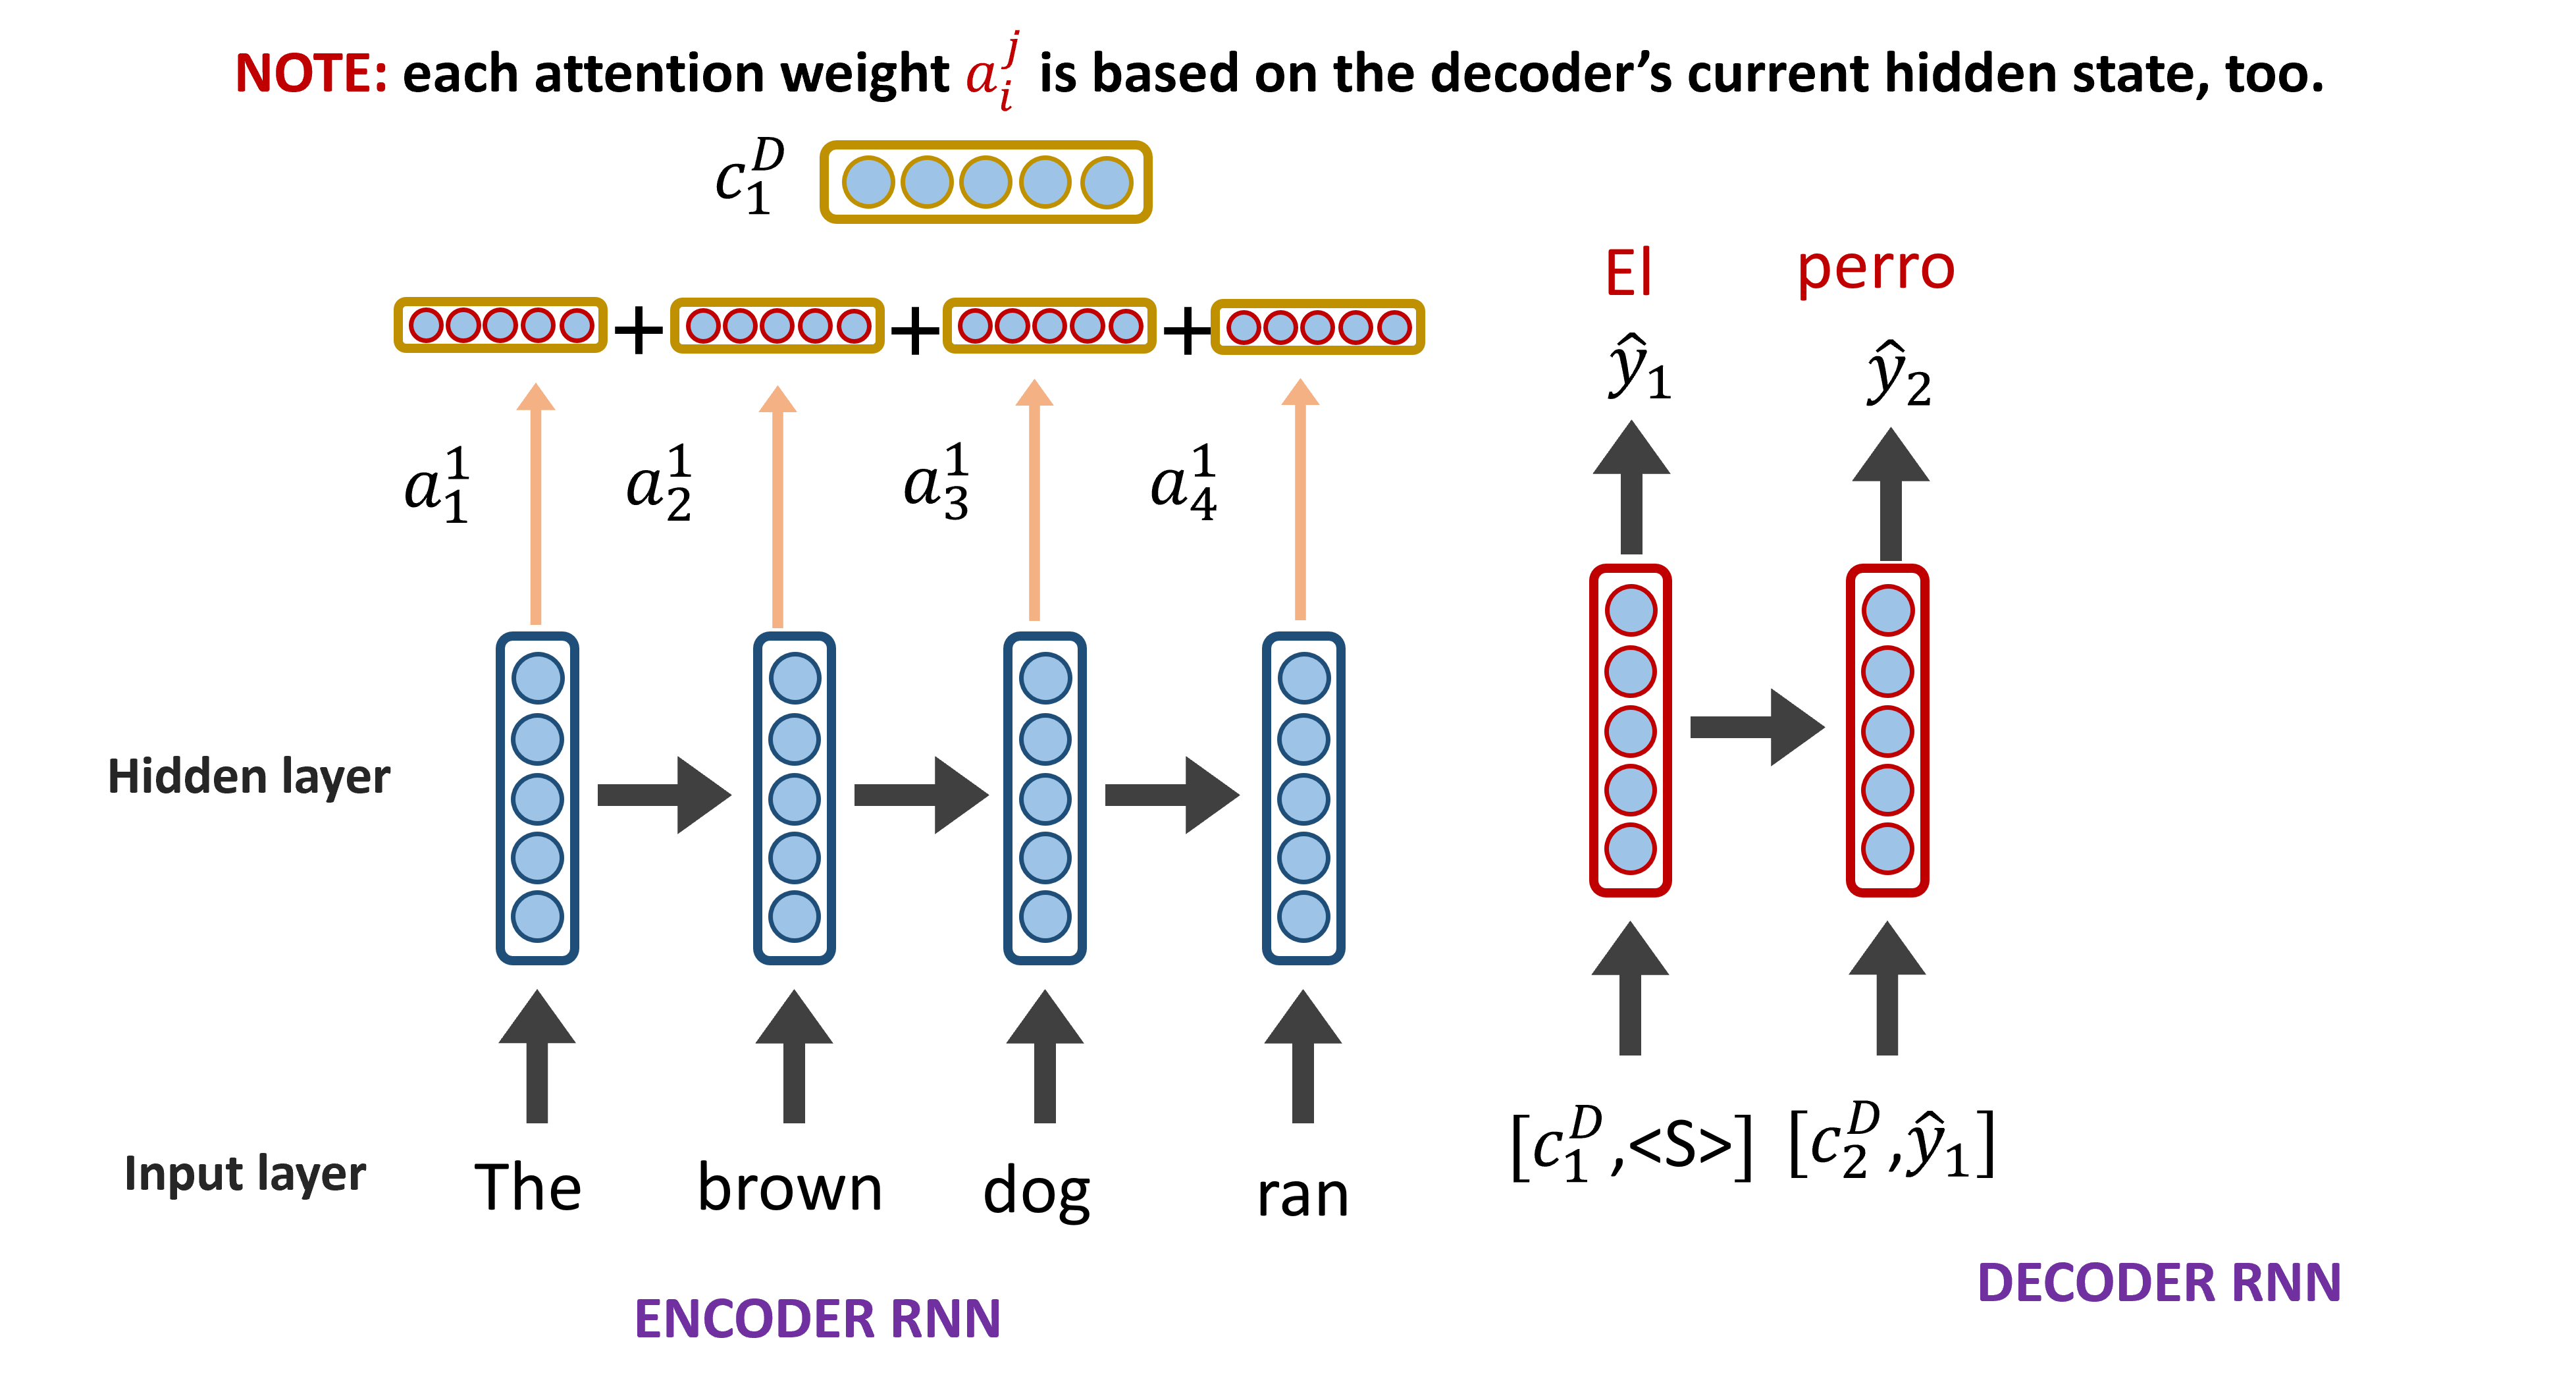
\includegraphics[width=0.8\linewidth,keepaspectratio]{bert29}
\end{center}	

\end{frame}

%%%%%%%%%%%%%%%%%%%%%%%%%%%%%%%%%%%%%%%%%%%%%%%%%%%%%%%%%%%
\begin{frame}[fragile]\frametitle{seq2seq + Attention}

\begin{center}
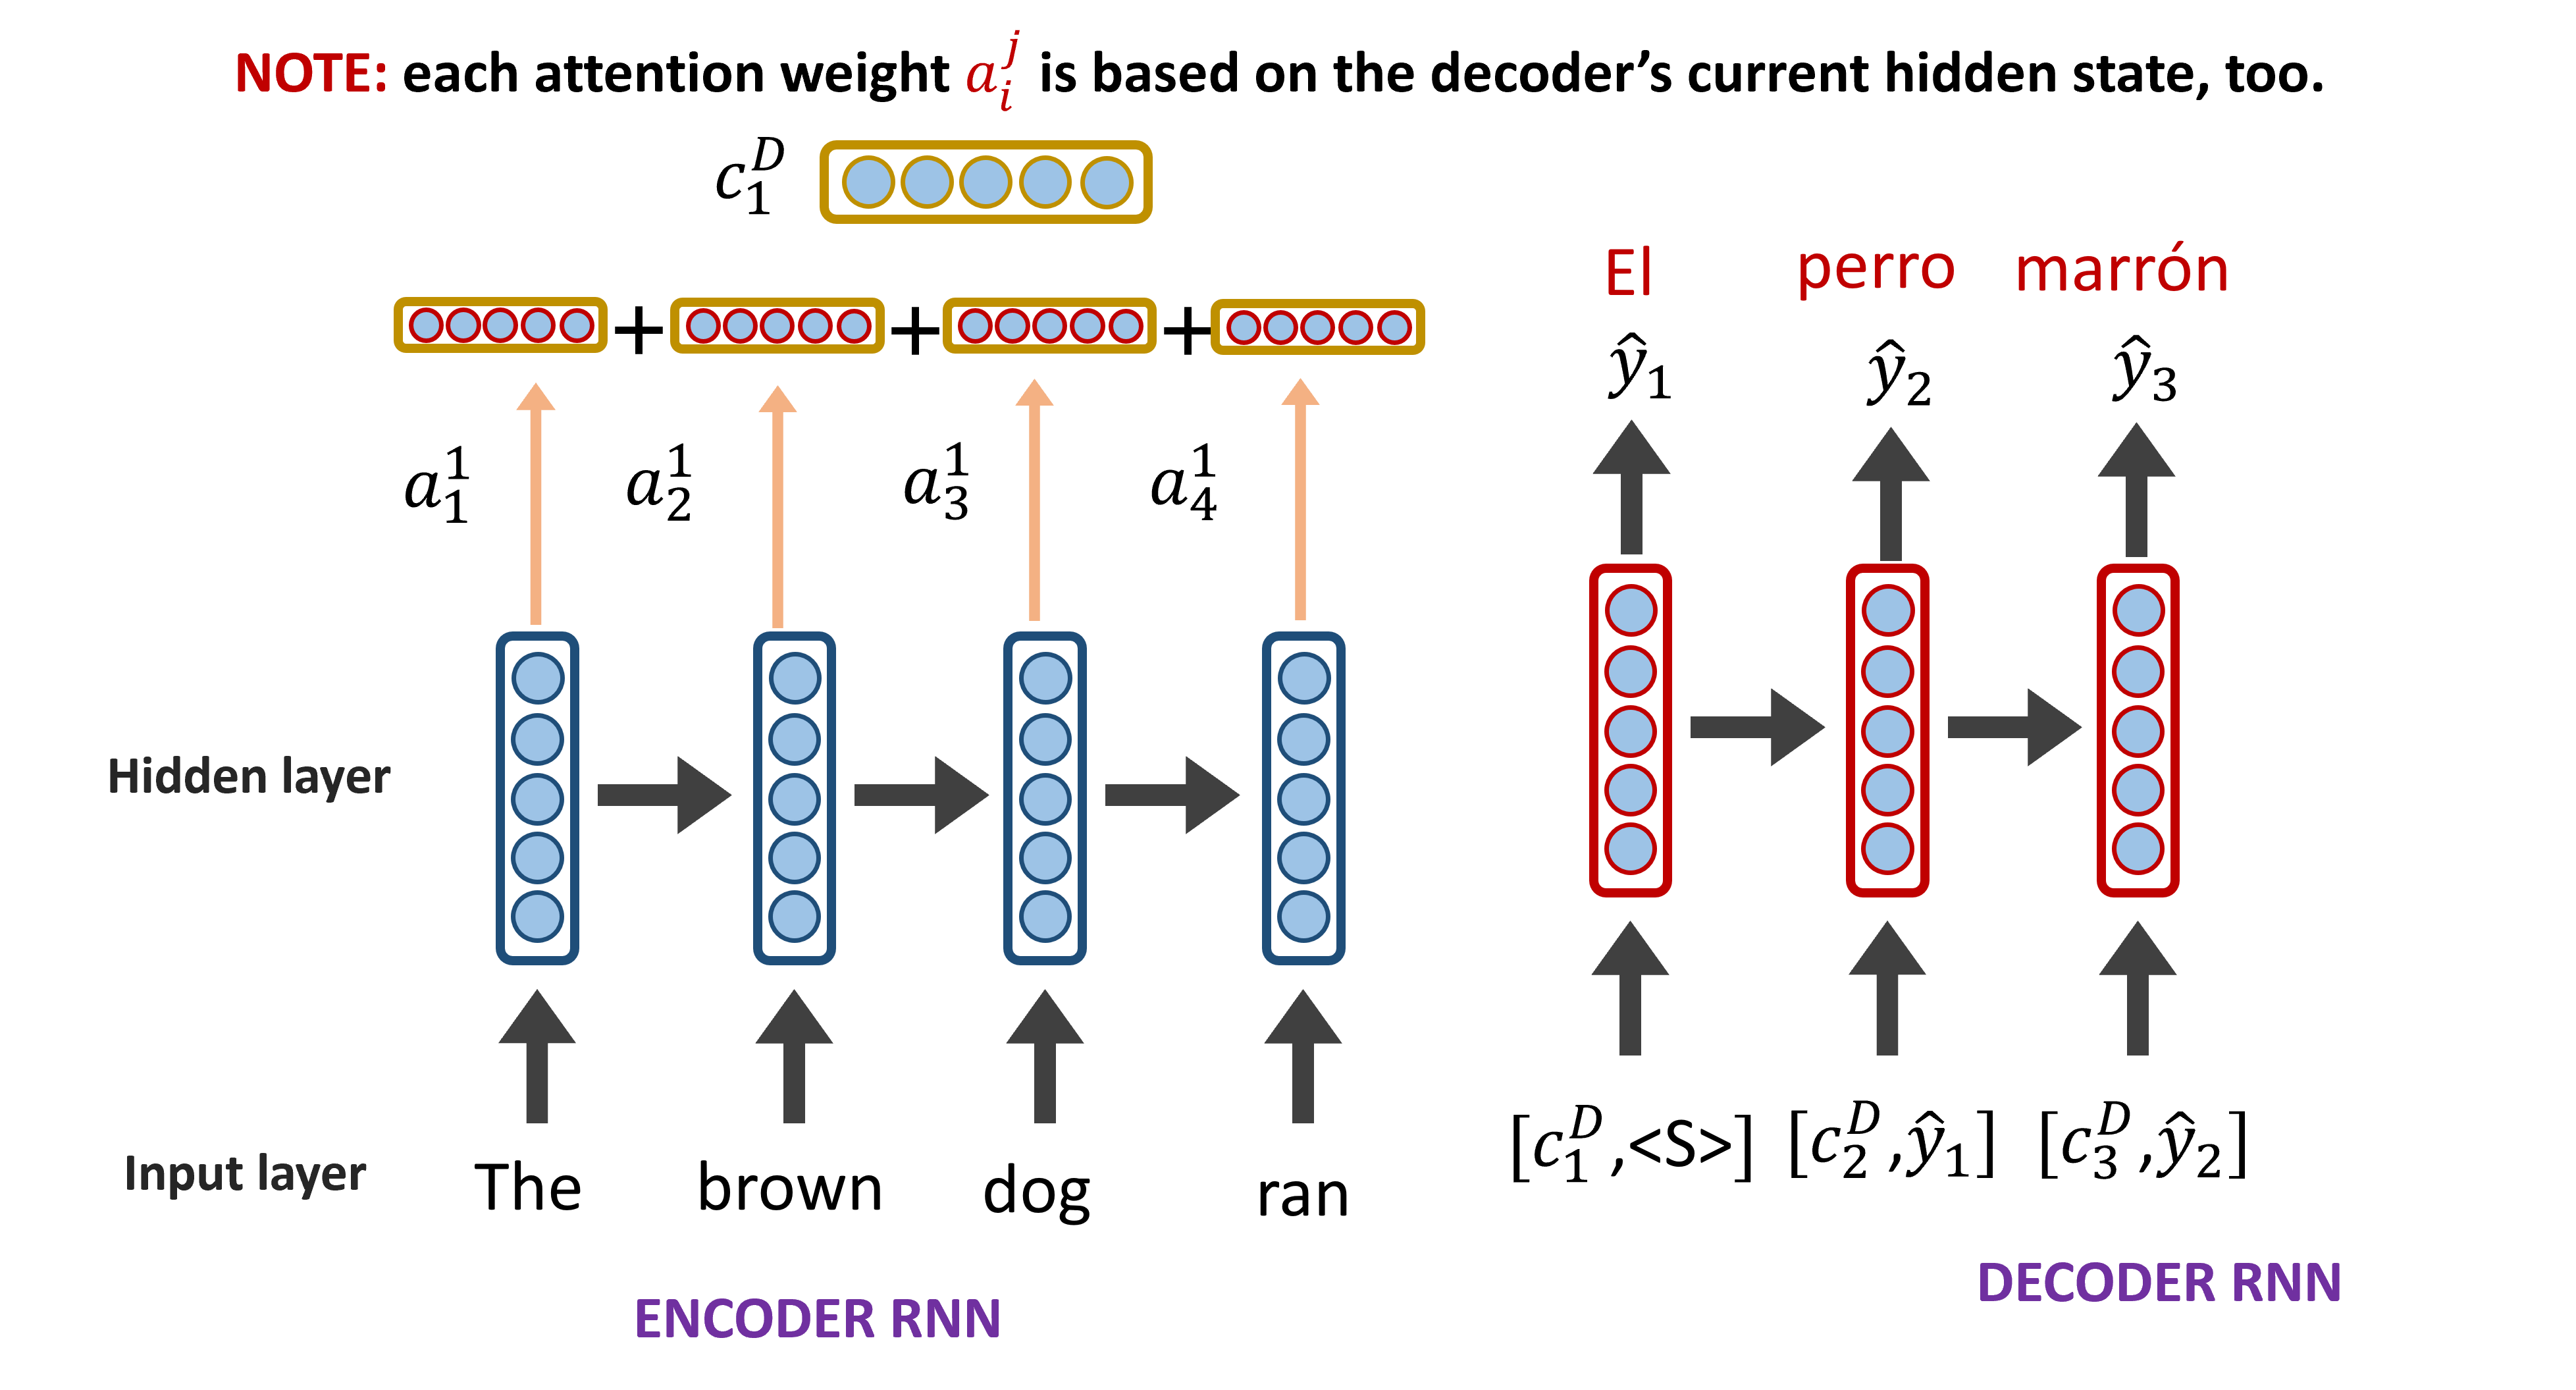
\includegraphics[width=0.8\linewidth,keepaspectratio]{bert30}
\end{center}	

\end{frame}

%%%%%%%%%%%%%%%%%%%%%%%%%%%%%%%%%%%%%%%%%%%%%%%%%%%%%%%%%%%
\begin{frame}[fragile]\frametitle{seq2seq + Attention}

\begin{center}
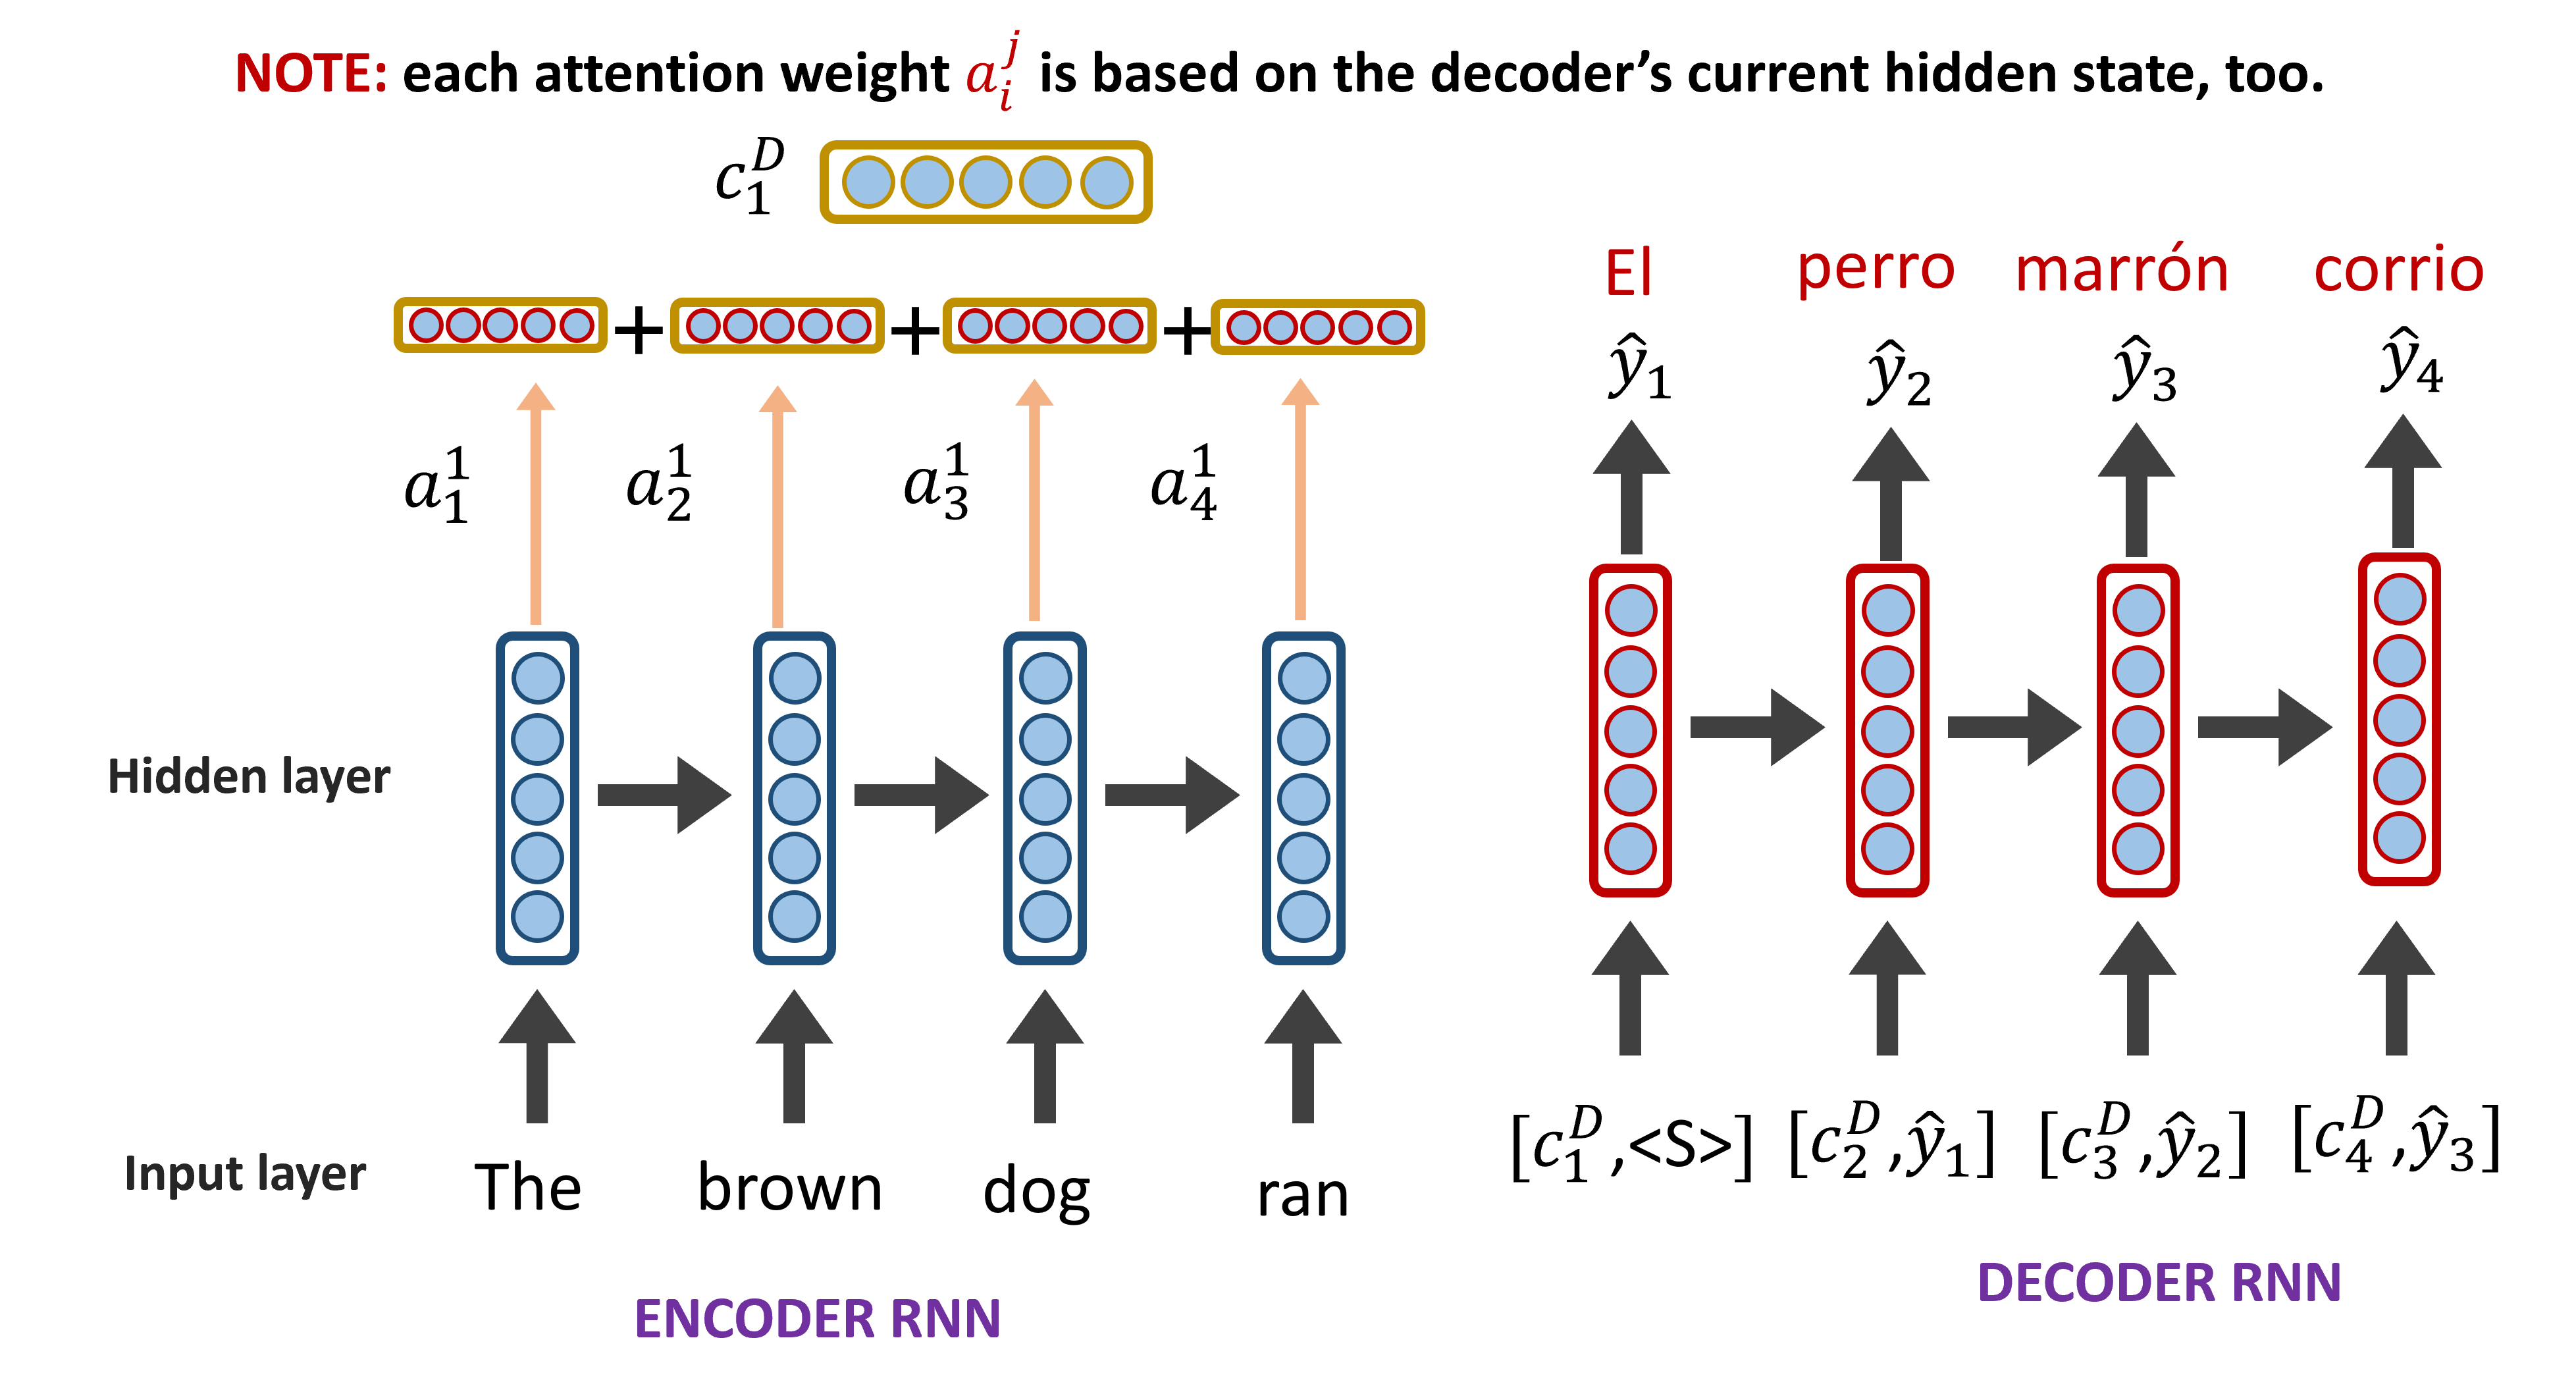
\includegraphics[width=0.8\linewidth,keepaspectratio]{bert31}
\end{center}	

\end{frame}

%%%%%%%%%%%%%%%%%%%%%%%%%%%%%%%%%%%%%%%%%%%%%%%%%%%%%%%%%%%
\begin{frame}[fragile]\frametitle{seq2seq + Attention}

\begin{center}
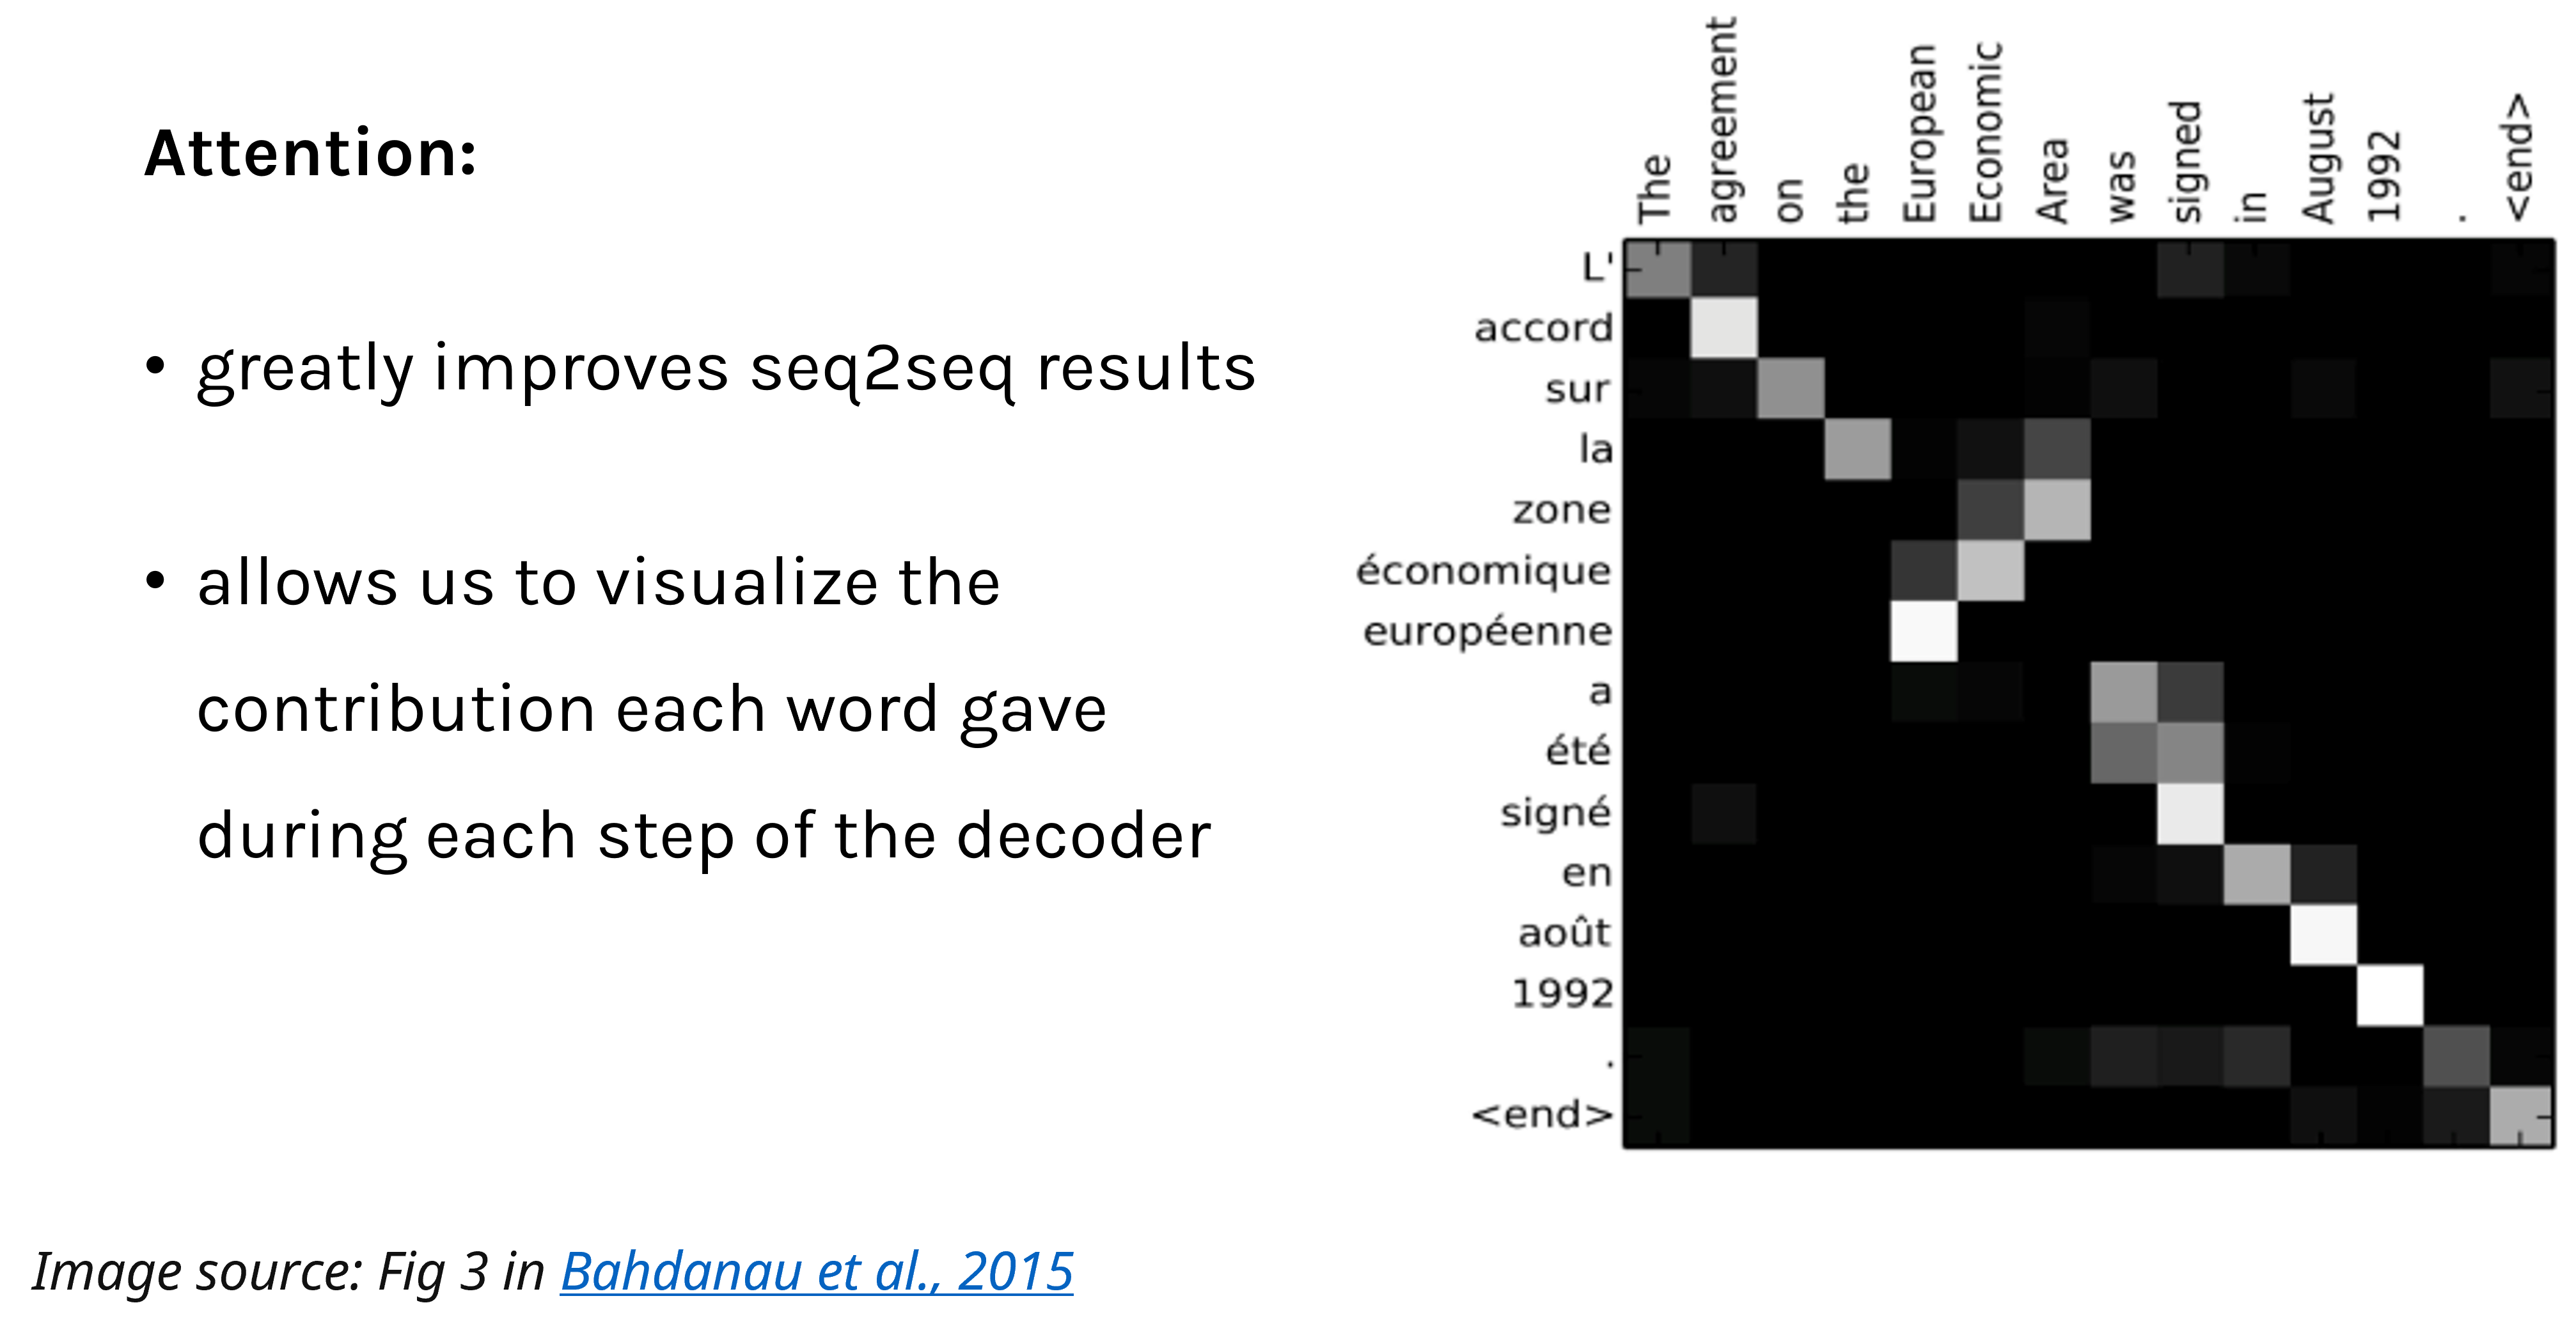
\includegraphics[width=\linewidth,keepaspectratio]{bert32}
\end{center}	

\end{frame}

% %%%%%%%%%%%%%%%%%%%%%%%%%%%%%%%%%%%%%%%%%%%%%%%%%%%%%%%%%%%%%%%%%%%%%%%%%%%%%%%%%%
% \begin{frame}[fragile]\frametitle{}
% \begin{center}
% {\Large Other Sentence Embeddings}
% \end{center}
% \end{frame}

% %%%%%%%%%%%%%%%%%%%%%%%%%%%%%%%%%%%%%%%%%%%%%%%%%%%%%%%%%%%
% \begin{frame}[fragile]\frametitle{ELMo: Embeddings from Language  Models}

% Deep contextualized word representations. Peters et al. NAACL 2018.  https://arxiv.org/abs/1802.05365

% \begin{itemize}
% \item ``Instead of using a fixed embedding for each word, ELMo looks at the entire sentence before assigning each word in it an embedding.''
% \item Breakout version of word token vectors or
% contextual word vectors
% \item Learn word token vectors using long contexts not context  windows (here, whole sentence, could be longer)
% \item Learn a deep Bi-NLM and use all its layers in prediction
% \end{itemize}

% % {\tiny (Ref: CS224n: Natural Language Processing with Deep Learning - Christopher Manning)}

% \end{frame}

% %%%%%%%%%%%%%%%%%%%%%%%%%%%%%%%%%%%%%%%%%%%%%%%%%%%%%%%%%%%
% \begin{frame}[fragile]\frametitle{ELMo: Embeddings from Language  Models}

% \begin{itemize}
% \item Train a bidirectional LM
% \item Aim at performant but not overly large LM:

% \begin{itemize}
% \item Use 2 biLSTM layers
% \item Use character CNN to build initial word representation 
% \item User 4096 dim hidden/cell LSTM states with 512 dim projections to next input
% \item Use a residual connection
% \item Tie parameters of token input and output (softmax) and tie these between forward and backward LMs
% \end{itemize}

% \end{itemize}

% % {\tiny (Ref: CS224n: Natural Language Processing with Deep Learning - Christopher Manning)}

% \end{frame}

% %%%%%%%%%%%%%%%%%%%%%%%%%%%%%%%%%%%%%%%%%%%%%%%%%%%%%%%%%%%
% \begin{frame}[fragile]\frametitle{ELMo used in a sequence tagger}

% \begin{center}
% 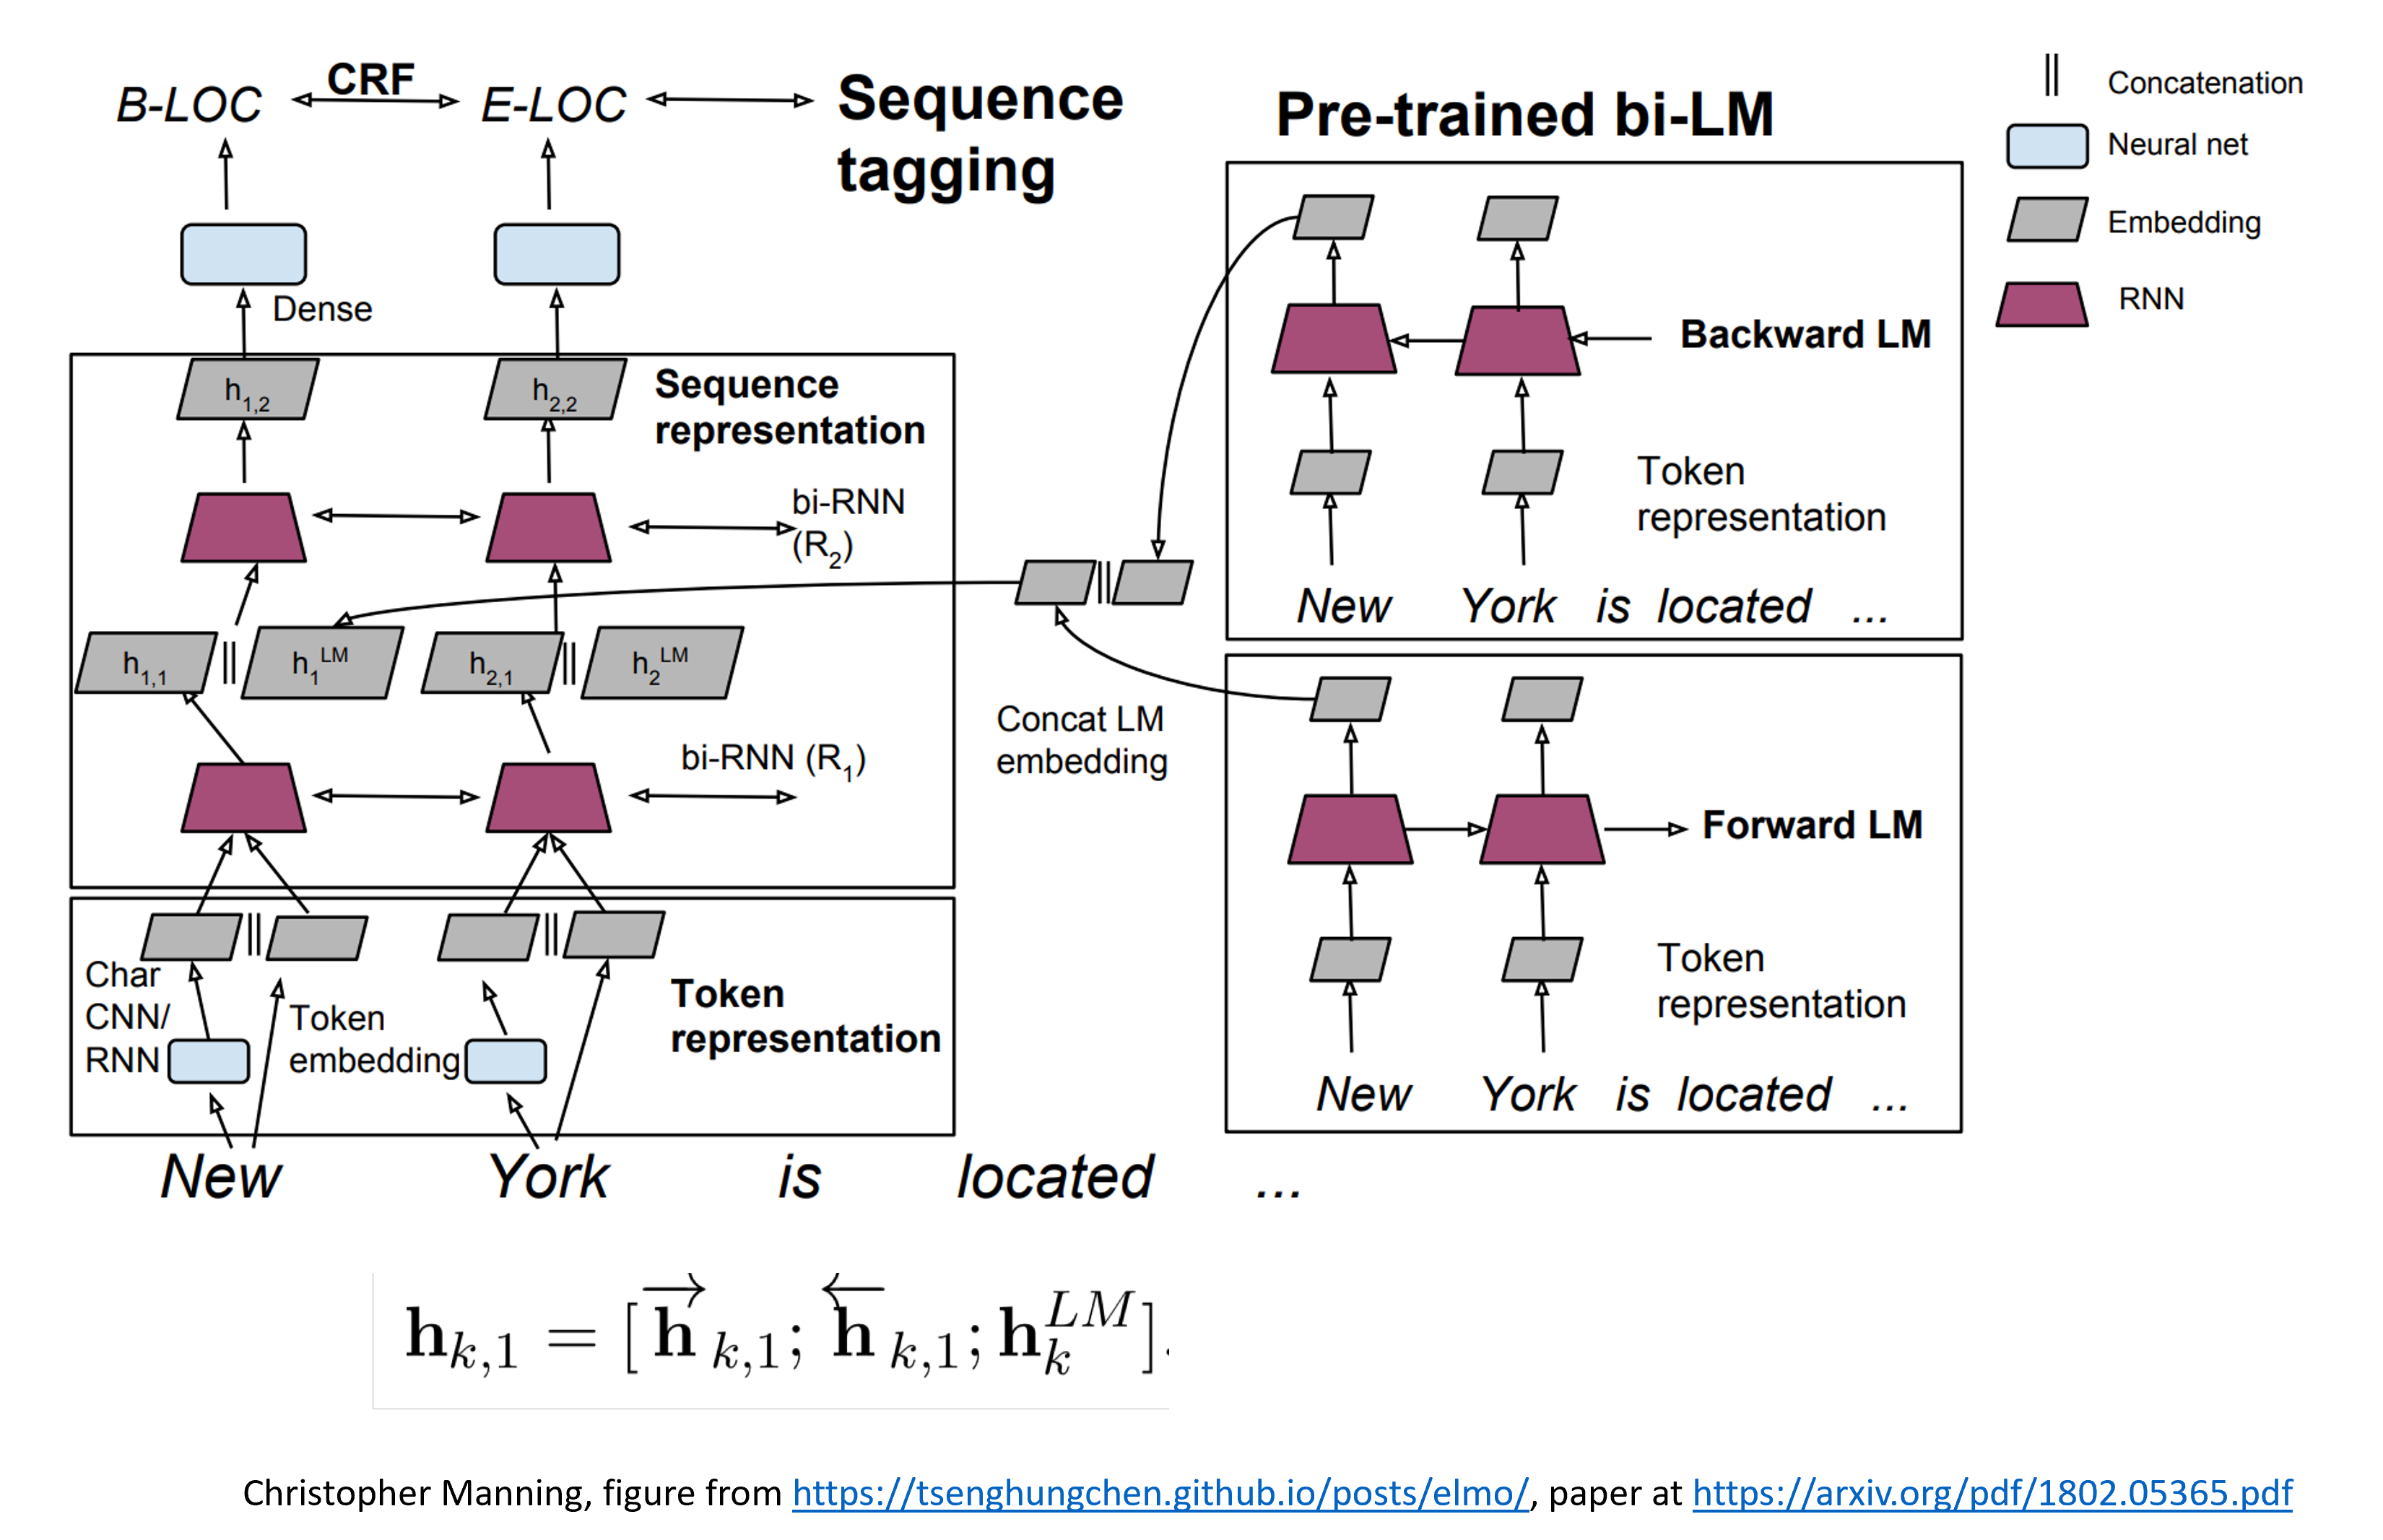
\includegraphics[width=\linewidth,keepaspectratio]{bert33}
% \end{center}	

% % {\tiny (Ref: CS224n: Natural Language Processing with Deep Learning - Christopher Manning)}

% \end{frame}

% %%%%%%%%%%%%%%%%%%%%%%%%%%%%%%%%%%%%%%%%%%%%%%%%%%%%%%%%%%%
% \begin{frame}[fragile]\frametitle{ELMo results: Great for all tasks}

% \begin{center}
% 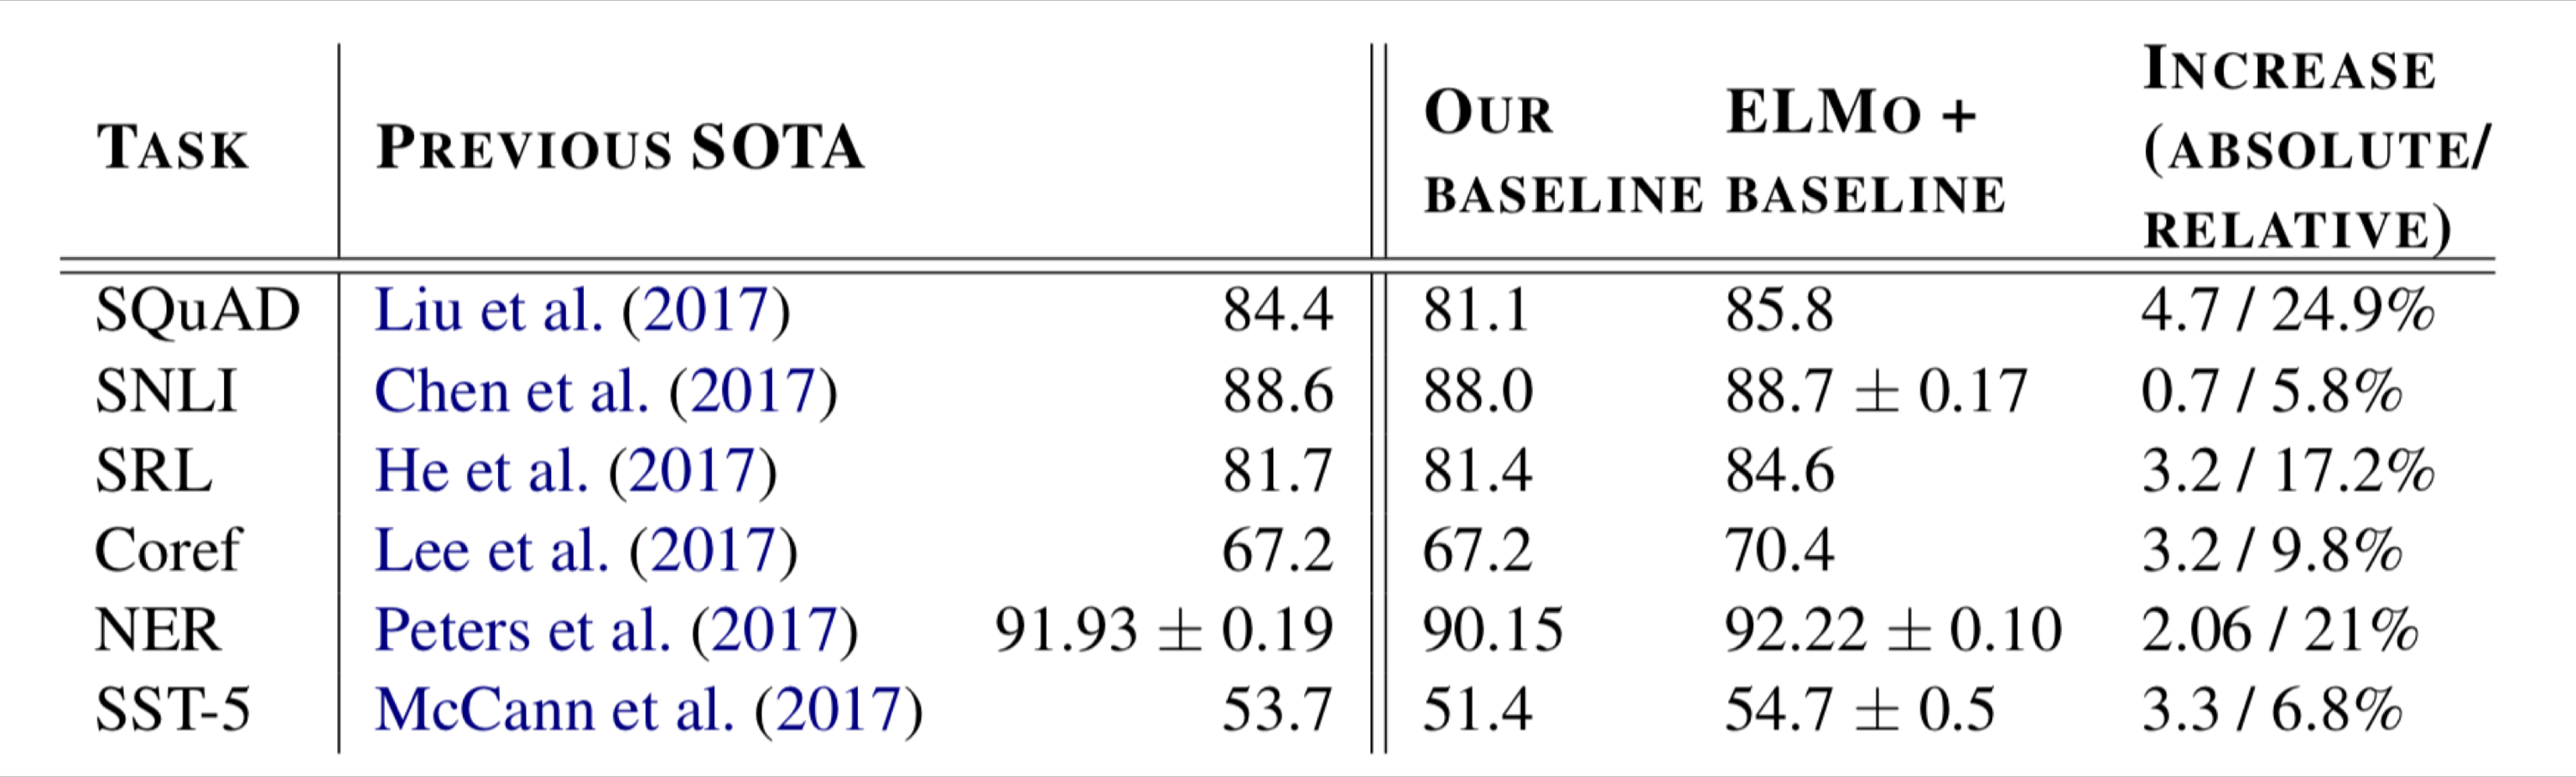
\includegraphics[width=\linewidth,keepaspectratio]{bert34}
% \end{center}	

% % {\tiny (Ref: CS224n: Natural Language Processing with Deep Learning - Christopher Manning)}

% \end{frame}

% %%%%%%%%%%%%%%%%%%%%%%%%%%%%%%%%%%%%%%%%%%%%%%%%%%%%%%%%%%%
% \begin{frame}[fragile]\frametitle{ELMo: Roles of different layers}

% The two biLSTM NLM layers have differentiated uses/meanings

% \begin{itemize}
% \item Lower layer is better for lower-level syntax, etc.
% Part-of-speech tagging, syntactic dependencies, NER
% \item Higher layer is better for higher-level semantics
% Sentiment, Semantic role labeling, question answering, SNLI

% \end{itemize}


% % {\tiny (Ref: CS224n: Natural Language Processing with Deep Learning - Christopher Manning)}

% \end{frame}


%%%%%%%%%%%%%%%%%%%%%%%%%%%%%%%%%%%%%%%%%%%%%%%%%%%%%%%%%%%
\begin{frame}[fragile]\frametitle{Self-Attention}


\begin{center}
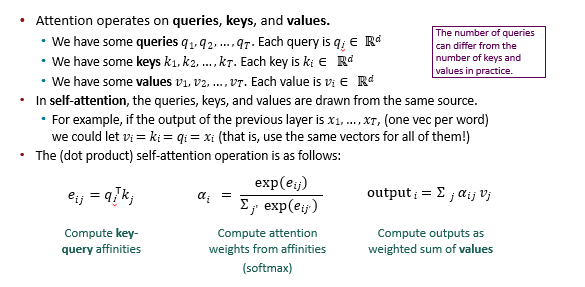
\includegraphics[width=\linewidth,keepaspectratio]{bert40}
\end{center}	

 
% {\tiny (Ref: Language \& Machine Learning - John Hewitt)}
\end{frame}

%%%%%%%%%%%%%%%%%%%%%%%%%%%%%%%%%%%%%%%%%%%%%%%%%%%%%%%%%%%
\begin{frame}[fragile]\frametitle{Self-Attention}


\begin{center}
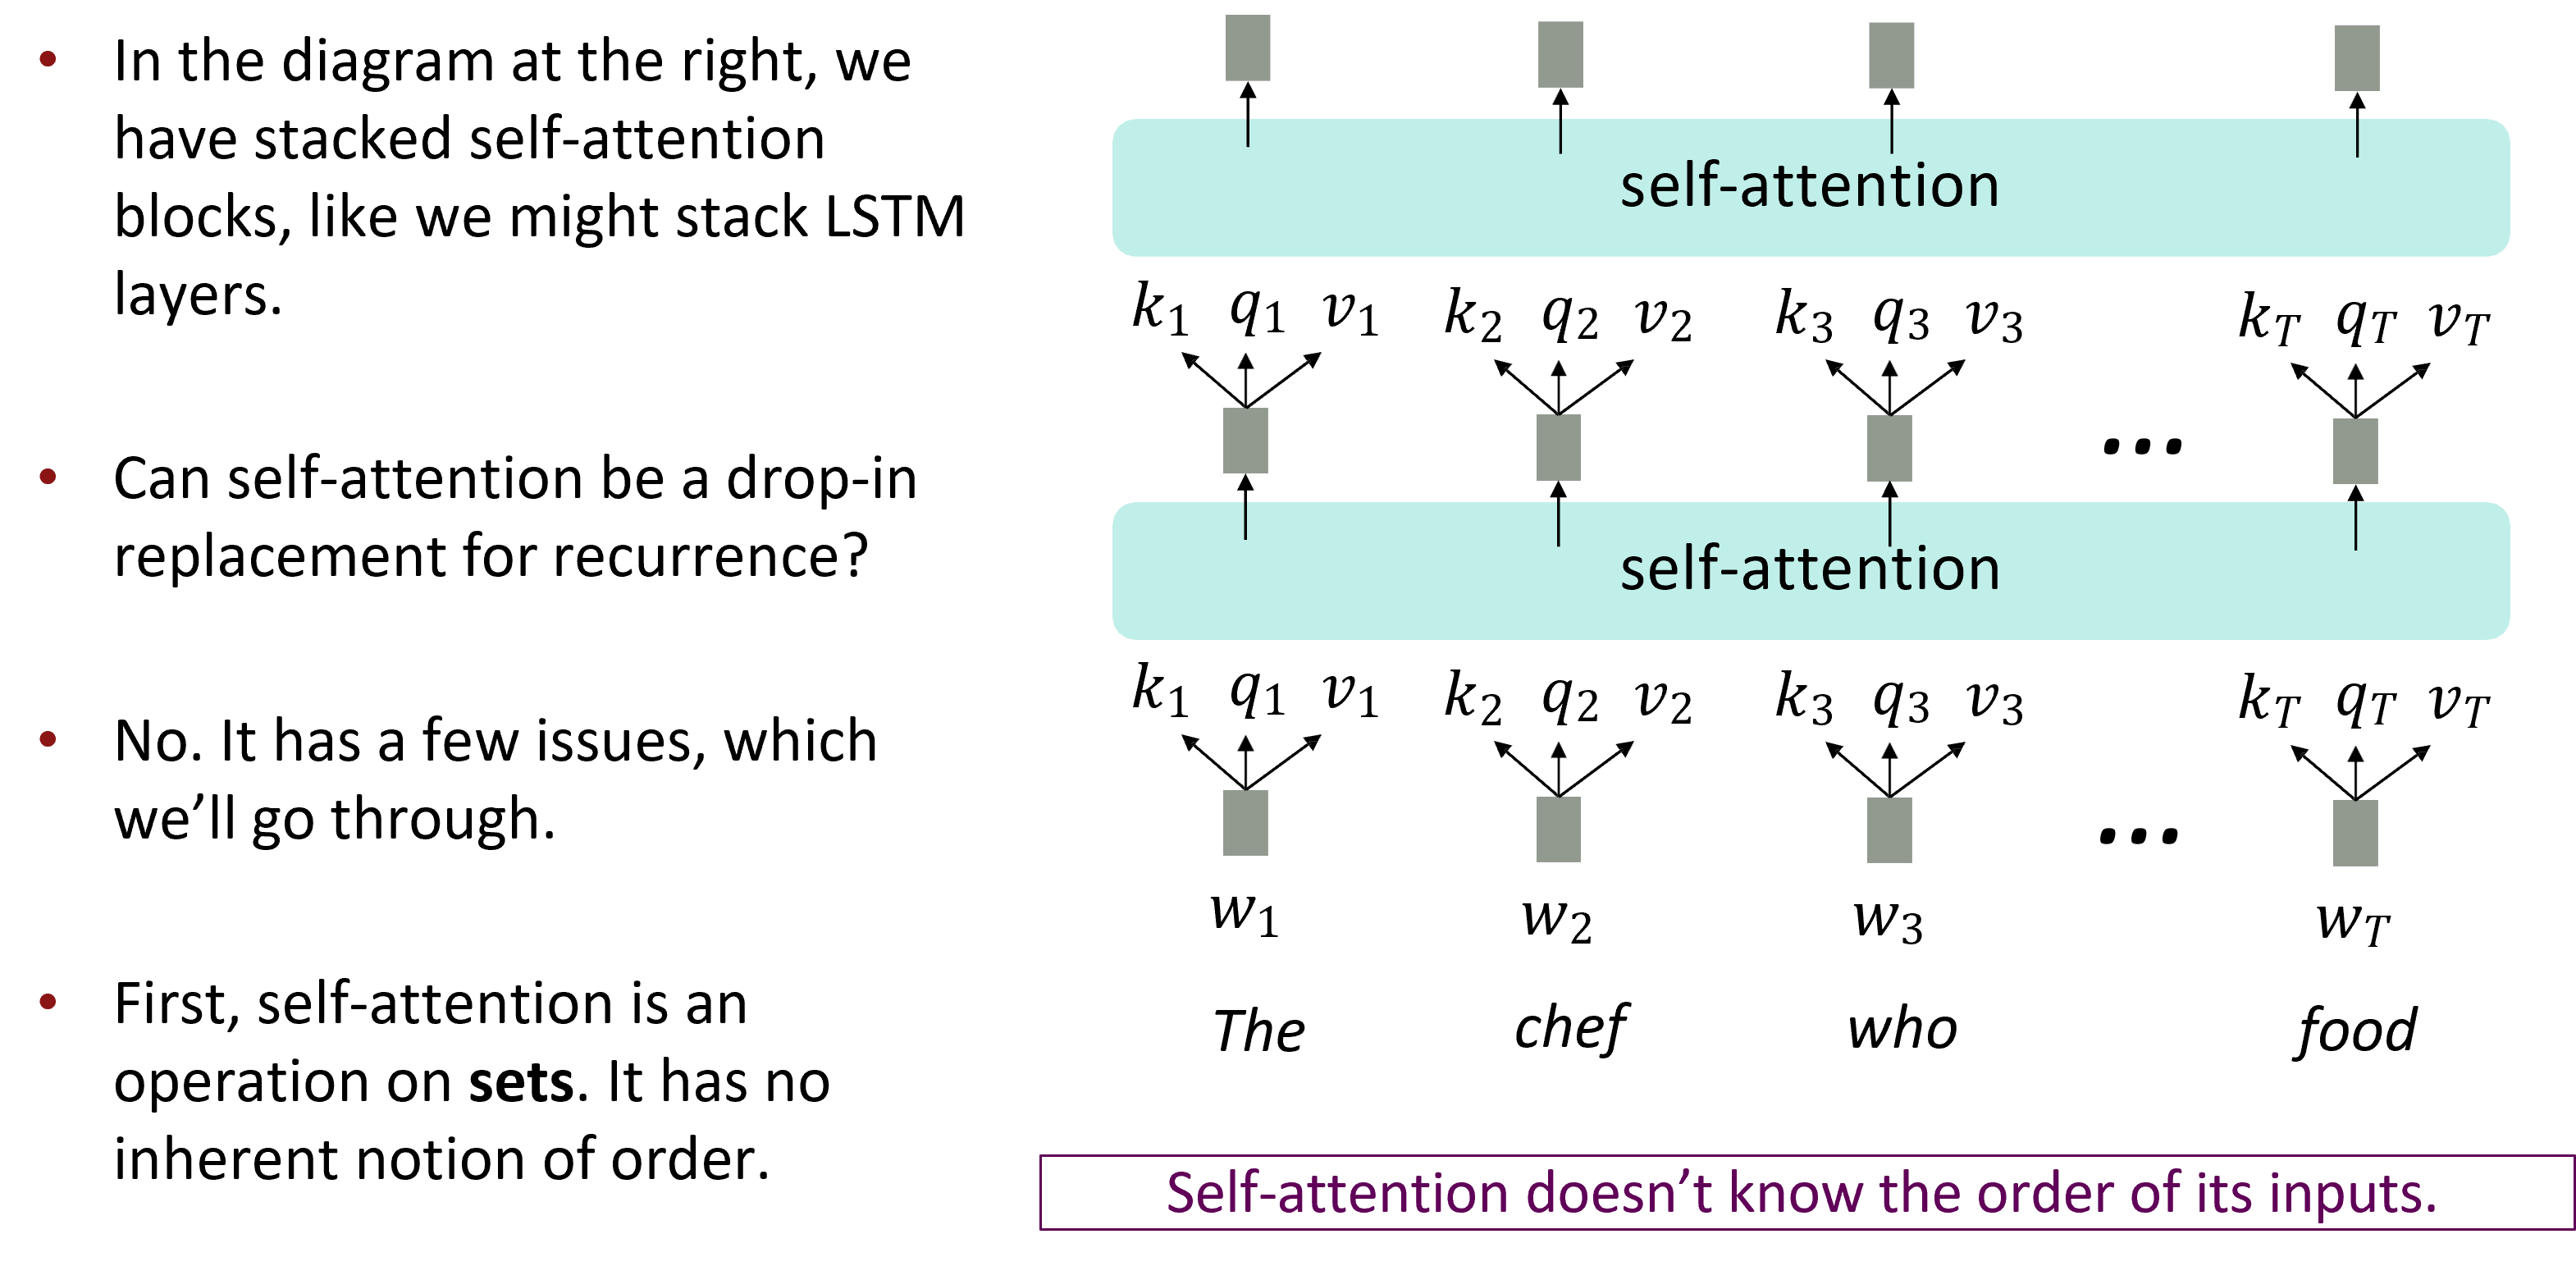
\includegraphics[width=\linewidth,keepaspectratio]{bert41}
\end{center}	

 
% {\tiny (Ref: Language \& Machine Learning - John Hewitt)}
\end{frame}

%%%%%%%%%%%%%%%%%%%%%%%%%%%%%%%%%%%%%%%%%%%%%%%%%%%%%%%%%%%
\begin{frame}[fragile]\frametitle{Self-Attention}

Barriers and solutions for Self-Attention as a building block

\begin{center}
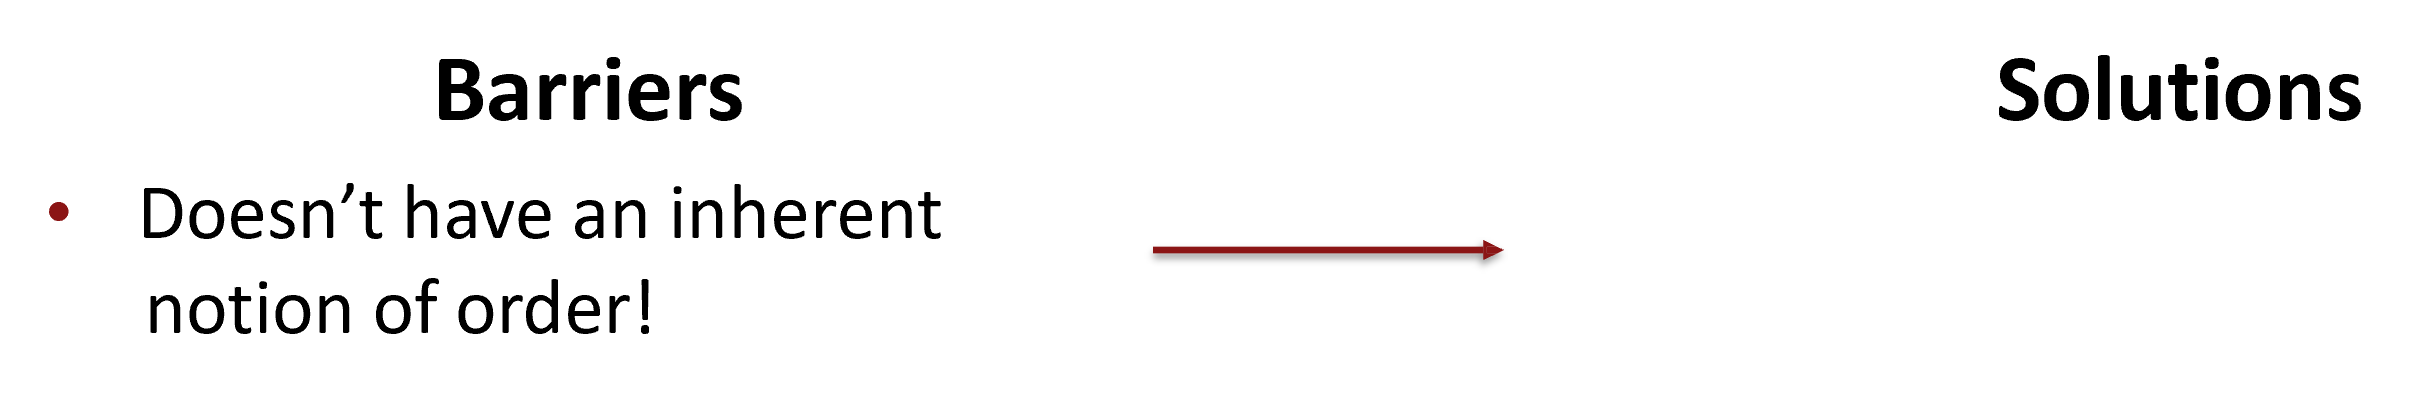
\includegraphics[width=\linewidth,keepaspectratio]{bert42}
\end{center}	

 
% {\tiny (Ref: Language \& Machine Learning - John Hewitt)}
\end{frame}

%%%%%%%%%%%%%%%%%%%%%%%%%%%%%%%%%%%%%%%%%%%%%%%%%%%%%%%%%%%
\begin{frame}[fragile]\frametitle{Self-Attention}

Fixing the first self-attention problem: Sequence order

\begin{center}
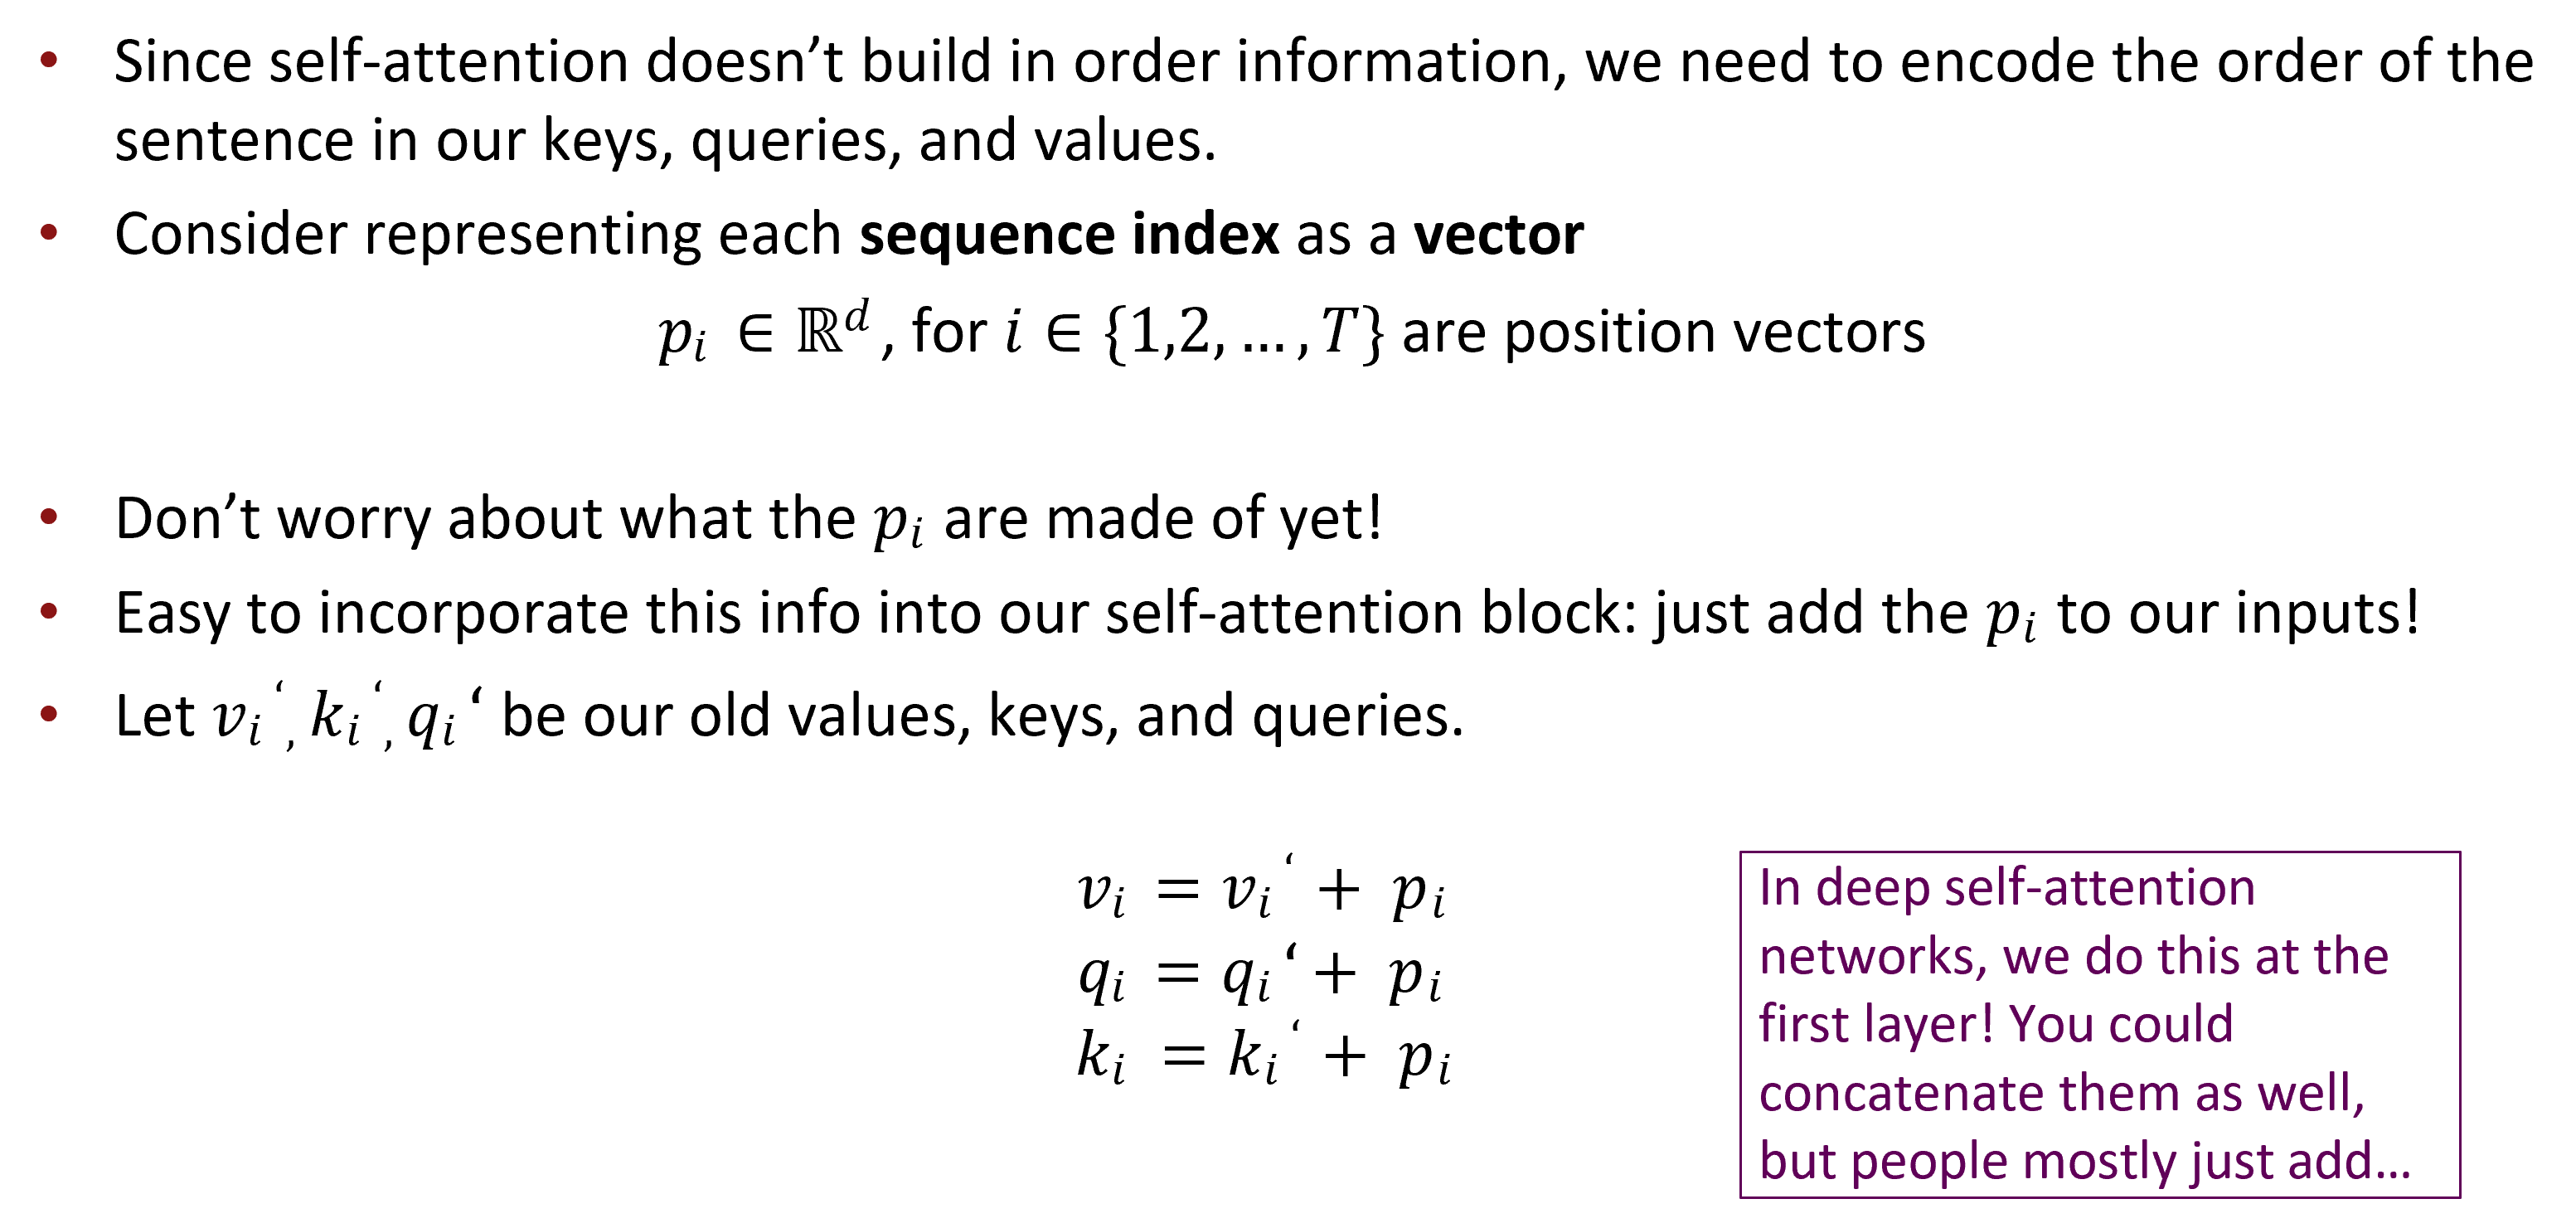
\includegraphics[width=\linewidth,keepaspectratio]{bert43}
\end{center}	

 
% {\tiny (Ref: Language \& Machine Learning - John Hewitt)}
\end{frame}

%%%%%%%%%%%%%%%%%%%%%%%%%%%%%%%%%%%%%%%%%%%%%%%%%%%%%%%%%%%
\begin{frame}[fragile]\frametitle{Self-Attention}

Position representation vectors through sinusoids

\begin{center}
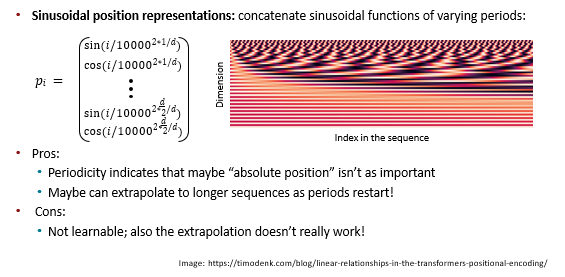
\includegraphics[width=\linewidth,keepaspectratio]{bert44}
\end{center}	

 
% {\tiny (Ref: Language \& Machine Learning - John Hewitt)}
\end{frame}

%%%%%%%%%%%%%%%%%%%%%%%%%%%%%%%%%%%%%%%%%%%%%%%%%%%%%%%%%%%
\begin{frame}[fragile]\frametitle{Self-Attention}

Barriers and solutions for Self-Attention as a building block

\begin{center}
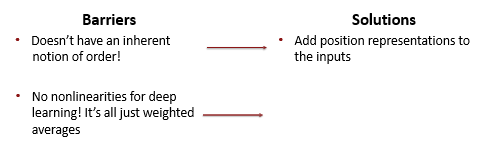
\includegraphics[width=\linewidth,keepaspectratio]{bert45}
\end{center}	

 
% {\tiny (Ref: Language \& Machine Learning - John Hewitt)}
\end{frame}

%%%%%%%%%%%%%%%%%%%%%%%%%%%%%%%%%%%%%%%%%%%%%%%%%%%%%%%%%%%
\begin{frame}[fragile]\frametitle{Self-Attention}

Adding nonlinearities in self-attention

\begin{center}
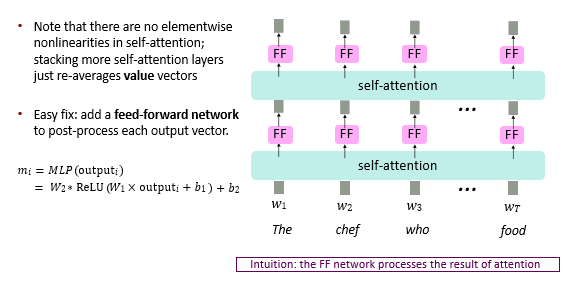
\includegraphics[width=\linewidth,keepaspectratio]{bert46}
\end{center}	

 
% {\tiny (Ref: Language \& Machine Learning - John Hewitt)}
\end{frame}

%%%%%%%%%%%%%%%%%%%%%%%%%%%%%%%%%%%%%%%%%%%%%%%%%%%%%%%%%%%
\begin{frame}[fragile]\frametitle{Self-Attention}

Barriers and solutions for Self-Attention as a building block

\begin{center}
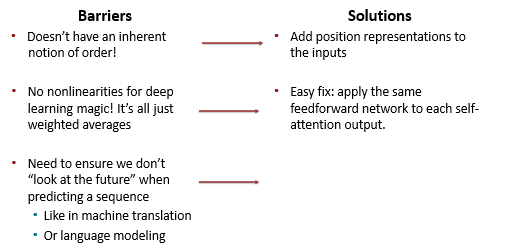
\includegraphics[width=\linewidth,keepaspectratio]{bert47}
\end{center}	

 
% {\tiny (Ref: Language \& Machine Learning - John Hewitt)}
\end{frame}


%%%%%%%%%%%%%%%%%%%%%%%%%%%%%%%%%%%%%%%%%%%%%%%%%%%%%%%%%%%
\begin{frame}[fragile]\frametitle{Self-Attention}

Masking the future in self-attention

\begin{center}
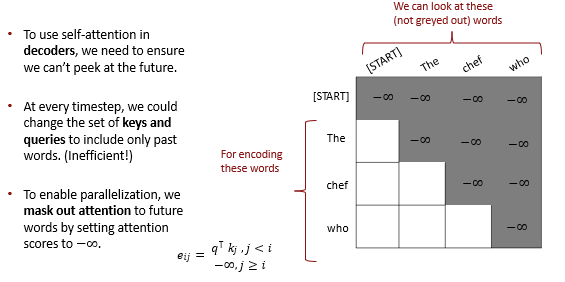
\includegraphics[width=\linewidth,keepaspectratio]{bert48}
\end{center}	

 
% {\tiny (Ref: Language \& Machine Learning - John Hewitt)}
\end{frame}

%%%%%%%%%%%%%%%%%%%%%%%%%%%%%%%%%%%%%%%%%%%%%%%%%%%%%%%%%%%
\begin{frame}[fragile]\frametitle{Self-Attention}

Barriers and solutions for Self-Attention as a building block

\begin{center}
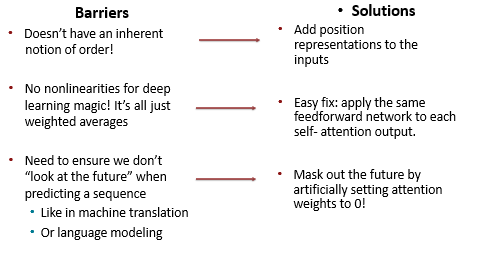
\includegraphics[width=\linewidth,keepaspectratio]{bert49}
\end{center}	

 
% {\tiny (Ref: Language \& Machine Learning - John Hewitt)}
\end{frame}

%%%%%%%%%%%%%%%%%%%%%%%%%%%%%%%%%%%%%%%%%%%%%%%%%%%%%%%%%%%
\begin{frame}[fragile]\frametitle{Self-Attention}

Necessities for a self-attention building block:

\begin{itemize}
\item Self-attention:
the basis of the method.
\item Position representations:
Specify the sequence order, since self-attention is an unordered function of its  inputs.
\item Nonlinearities:
\begin{itemize}
\item At the output of the self-attention block
\item Frequently implemented as a simple feed-forward network.
\end{itemize}	 

\item Masking:
\begin{itemize}
\item In order to parallelize operations while not looking at the future.
\item Keeps information about the future from “leaking” to the past.
\end{itemize}	 

\item That’s it! But this is not the Transformer model we’ve been hearing about.


\end{itemize}	 

 
% {\tiny (Ref: Language \& Machine Learning - John Hewitt)}
\end{frame}
